\documentclass[10pt,letterpaper,final,twoside,notitlepage]{article}
\usepackage[margin=.5in]{geometry} % 1/2 inch margins on all pages
\usepackage[utf8]{inputenc} % Define the input encoding
\usepackage[USenglish]{babel} % Define language used
\usepackage{amsmath,amsfonts,amssymb}
\usepackage{amsthm} % Gives us plain, definition, and remark to use in \theoremstyle{style}
\usepackage{mathtools} % Allow for text and math in align* environment.
\usepackage{thmtools}
\usepackage{thm-restate}
\usepackage{graphicx}

\usepackage[
backend=biber,
style=alphabetic,
citestyle=authoryear]{biblatex} % Must include citation somewhere in document to print bibliography
\usepackage{hyperref} % Generate hyperlinks to referenced items
\usepackage[nottoc]{tocbibind} % Prints the Reference/Bibliography in TOC as well
\usepackage[noabbrev,nameinlink]{cleveref} % Fancy cross-references in the document everywhere
\usepackage{nameref} % Can make references by name to places
\usepackage{caption} % Allows for greater control over captions in figure, algorithm, table, etc. environments
\usepackage{subcaption} % Allows for multiple figures in one Figure environment
\usepackage[binary-units=true]{siunitx} % Gives us ways to typeset units for stuff
\usepackage{csquotes} % Context-sensitive quotation facilities
\usepackage{enumitem} % Provides [noitemsep, nolistsep] for more compact lists
\usepackage{chngcntr} % Allows us to tamper with the counter a little more
\usepackage{empheq} % Allow boxing of equations in special math environments
\usepackage[x11names]{xcolor} % Gives access to coloring text in environments or just text, MUST be before tikz
\usepackage{tcolorbox} % Allows us to create boxes of various types for examples
\usepackage{tikz} % Allows us to create TikZ and PGF Pictures
\usepackage{ctable} % Greater control over tables and how they look
\usepackage{diagbox} % Allow us to have shared diagonal cells in tables
\usepackage{multirow} % Allow us to have a single cell in a table span multiple rows
\usepackage{titling} % Put document information throughout the document programmatically
\usepackage[linesnumbered,ruled,vlined]{algorithm2e} % Allows us to write algorithms in a nice style.

\counterwithin{figure}{section}
\counterwithin{table}{section}
\counterwithin{equation}{section}
\counterwithin{algocf}{section}
\crefname{algocf}{algorithm}{algorithms}
\Crefname{algocf}{Algorithm}{Algorithms}
\setcounter{secnumdepth}{4}
\setcounter{tocdepth}{4} % Include \paragraph in toc
\crefname{paragraph}{paragraph}{paragraphs}
\Crefname{paragraph}{Paragraph}{Paragraphs}

% Create a theorem environment
\theoremstyle{plain}
\newtheorem{theorem}{Theorem}[section]
% Create a numbered theorem-like environment for lemmas
\newtheorem{lemma}{Lemma}[theorem]

% Create a definition environment
\theoremstyle{definition}
\newtheorem{definition}{Defn}
\newtheorem{corollary}{Corollary}[section]
% \begin{definition}[Term] \label{def:}
%   Make sure the term is emphasized with \emph{term}.
%   This ensures that if \emph is changed, it shows up everywhere
% \end{definition}

% Create a numbered remark environment numbered based on definition
% NOTE: This version of remark MUST go inside a definition environment
\theoremstyle{remark}
\newtheorem{remark}{Remark}[definition]
%\counterwithin{definition}{subsection} % Uncomment to have definitions use section.subsection numbering

% Create an unnumbered remark environment for general use
% NOTE: This version of remark has NO restrictions on placement
\newtheorem*{remark*}{Remark}

% Create a special list that handles properties. It can be broken and restarted
\newlist{propertylist}{enumerate}{1} % {Name}{Template}{Max Depth}
% [newlistname, LevelsToApplyTo]{formatting options}
\setlist[propertylist, 1]{label=\textbf{(\roman*)}, ref=\textbf{(\roman*)}, noitemsep, nolistsep}
\crefname{propertylisti}{property}{properties}
\Crefname{propertylisti}{Property}{Properties}

% Create a special list that handles enumerate starting with lower letters. Breakable/Restartable.
\newlist{boldalphlist}{enumerate}{1} % {Name}{Template}{Max Depth}
% [newlistname, LevelsToApplyTo]{formatting options}
\setlist[boldalphlist, 1]{label=\textbf{(\alph*)}, ref=\alph*, noitemsep, nolistsep} % Set options

\newlist{nocrefenumerate}{enumerate}{1} % {Name}{Template}{Max Depth}
% [newlistname, LevelsToApplyTo]{formatting options}
\setlist[nocrefenumerate, 1]{label=(\arabic*), ref=(\arabic*), noitemsep, nolistsep}

% Create a list that allows for deeper nesting of numbers. By default enumerate only allows depth=4.
\newlist{nestednums}{enumerate}{6}
% [newlistname, LevelsToApplyTo]{formatting options}
\setlist[nestednums]{noitemsep, label*=\arabic*.}

\tcbuselibrary{breakable} % Allow tcolorboxes to be broken across pages
% Create a tcolorbox for examples
% /begin{example}[extra name]{NAME}
% Create a tcolorbox for examples
% Argument #1 is optional, given by [], that is the textbook's problem number
% Argument #2 is mandatory, given by {}, that is the title for the example
% Avoid putting special characters, (), [], {}, ",", etc. in the title.
\newtcolorbox[auto counter,
number within=section,
number format=\arabic,
crefname={example}{examples}, % Define reference format for cref (No Capitals)
Crefname={Example}{Examples}, % Reference format for cleveref (With Capitals)
]{example}[2][]{ % The [2][] Means the first argument is optional
  width=\textwidth,
  title={Example \thetcbcounter: #2. #1}, % Parentheses and commas are not well supported
  fonttitle=\bfseries,
  label={ex:#2},
  nameref=#2,
  colbacktitle=white!100!black,
  coltitle=black!100!white,
  colback=white!100!black,
  upperbox=visible,
  lowerbox=visible,
  sharp corners=all,
  breakable
}

% Create a tcolorbox for general use
\newtcolorbox[% auto counter,
% number within=section,
% number format=\arabic,
% crefname={example}{examples}, % Define reference format for cref (No Capitals)
% Crefname={Example}{Examples}, % Reference format for cleveref (With Capitals)
]{blackbox}{
  width=\textwidth,
  % title={},
  fonttitle=\bfseries,
  % label={},
  % nameref=,
  colbacktitle=white!100!black,
  coltitle=black!100!white,
  colback=white!100!black,
  upperbox=visible,
  lowerbox=visible,
  sharp corners=all
}

% Redefine the 'end of proof' symbol to be a black square, not blank
\renewcommand{\qedsymbol}{$\blacksquare$} % Change proofs to have black square at end

% Common Mathematical Stuff
\newcommand{\Abs}[1]{\ensuremath{\lvert #1 \rvert}}
\newcommand{\DNE}{\ensuremath{\mathrm{DNE}}} % Used when limit of function Does Not Exist

% Complex Numbers functions
\renewcommand{\Re}{\operatorname{Re}} % Redefine to use the command, but not the fraktur version
\renewcommand{\Im}{\operatorname{Im}} % Redefine to use the command, but not the fraktur version
\newcommand{\Real}[1]{\ensuremath{\Re \lbrace #1 \rbrace}}
\newcommand{\Imag}[1]{\ensuremath{\Im \lbrace #1 \rbrace}}
\newcommand{\Conjugate}[1]{\ensuremath{\overline{#1}}}
\newcommand{\Modulus}[1]{\ensuremath{\lvert #1 \rvert}}
\DeclareMathOperator{\PrincipalArg}{\ensuremath{Arg}}

% Math Operators that are useful to abstract the written math away to one spot
% Number Sets
\DeclareMathOperator{\RealNumbers}{\ensuremath{\mathbb{R}}}
\DeclareMathOperator{\AllIntegers}{\ensuremath{\mathbb{Z}}}
\DeclareMathOperator{\PositiveInts}{\ensuremath{\mathbb{Z}^{+}}}
\DeclareMathOperator{\NegativeInts}{\ensuremath{\mathbb{Z}^{-}}}
\DeclareMathOperator{\NaturalNumbers}{\ensuremath{\mathbb{N}}}
\DeclareMathOperator{\ComplexNumbers}{\ensuremath{\mathbb{C}}}
\DeclareMathOperator{\RationalNumbers}{\ensuremath{\mathbb{Q}}}

% Calculus operators
\DeclareMathOperator*{\argmax}{argmax} % Thin Space and subscripts are UNDER in display

% Signal and System Functions
\DeclareMathOperator{\UnitStep}{\mathcal{U}}
\DeclareMathOperator{\sinc}{sinc} % sinc(x) = (sin(pi x)/(pi x))

% Transformations
\DeclareMathOperator{\Lapl}{\mathcal{L}} % Declare a Laplace symbol to be used

% Logical Operators
\DeclareMathOperator{\XOR}{\oplus}

% x86 CPU Registers
\newcommand{\rbpRegister}{\texttt{\%rbp}}
\newcommand{\rspRegister}{\texttt{\%rsp}}
\newcommand{\ripRegister}{\texttt{\%rip}}
\newcommand{\raxRegister}{\texttt{\%rax}}
\newcommand{\rbxRegister}{\texttt{\%rbx}}

%%% Local Variables:
%%% mode: latex
%%% TeX-master: shared
%%% End:


% These packages are more specific to certain documents, but will be availabe in the template
% \usepackage{esint} % Provides us with more types of integral symbols to use
\usepackage[outputdir=./TeX_Output]{minted} % Allow us to nicely typeset 300+ programming languages
% This document must be compiled with the -shell-escape flag if the packages above are uncommented

\graphicspath{{./Drawings/EDAF35-Operating_Systems/}} % Uncomment this to use pictures in this document
\addbibresource{./Bibliographies/EDAF35-Operating_Systems.bib}

% Math Operators that are useful to abstract the written math away to one spot
% These are supposed to be document-specific mathematical operators that will make life easier
% Many fundamental operators are defined in Reference_Sheet_Preamble.tex

\usemintedstyle{emacs} % Best for use on white backgrounds. Use for inline-code
% This macro creates the 2 minted environments for kernel source code with common options
\def\mintedkernelargs{
  frame=lines, % Surround the source code with lines on top and bottom
  linenos, % We want to show line numbers for each line in the margin
  % Colors used here are xcolor X11 colors.
  % style=fruity, % Use the fruity color scheme. Best for use on black backgrounds. Use for code blocks.
  % bgcolor=black, % Set the background used
  style=emacs,
  bgcolor=white,
  autogobble=true, % Automatically remove shared indentation from files
  breaklines=true, % Break lines that are too long at convenient locations
}
\newcommand{\makenewmintedfiles}[1]{
  \newminted[kernelsource]{c}{#1} % Use with \begin{kernelsource} code \end{kernelsource}

  \newmintedfile[kernelsourcefile]{c}{#1} % Use with \kernelsourcefile[additional-options]{Filename}
}
\expandafter\makenewmintedfiles\expandafter{\mintedkernelargs}
\newmintinline[kernelinline]{c}{% Use with \kernelinline{code}
  style=emacs,
  bgcolor=white,
}

\DeclareSIUnit{\rpm}{RPM}

\DeclareMathOperator{\Messages}{\mathcal{M}}
\DeclareMathOperator{\Ciphertexts}{\mathcal{C}}
\DeclareMathOperator{\Keyspace}{\mathcal{K}}
\DeclareMathOperator{\Authenticators}{\mathcal{A}}

\begin{titlepage}
  \title{EDAF35: Operating Systems --- Reference Sheet \\ Lund University}
  \author{Karl Hallsby}
  \date{Last Edited: \today} % We want to inform people when this document was last edited
\end{titlepage}

\begin{document}
\pagenumbering{gobble}
\maketitle
\pagenumbering{roman} % i, ii, iii on beginning pages, that don't have content
\tableofcontents
\clearpage
\listoftheorems[ignoreall, show={definition, Definition}]
\clearpage
\pagenumbering{arabic} % 1,2,3 on content pages

\nocite{*}

\section{Operating System Introduction}\label{sec:OS_Intro}
A computer system can be roughly divided into 4 parts.
\begin{itemize}[noitemsep]
\item The \nameref{def:Hardware}
\item The \nameref{def:Operating_System}
\item The \nameref{def:Application_Program}s
\item The Users
\end{itemize}

\begin{definition}[Hardware]\label{def:Hardware}
  \emph{Hardware} is the physical components of the system and provide the basic computing resources for the system..
  Hardware includes the \nameref{def:CPU}, \nameref{def:Memory}, and all I/O devices (monitor, keyboard, mouse, etc.).

  \begin{remark}[How to Differentiate]\label{rmk:Hardware_Differentiate}
    If you are finding it difficult to tell \nameref{def:Hardware}, \nameref{def:Software}, and \nameref{def:Firmware} apart, answer this simple question.
    Can you hit it with a hammer and break the thing?
    \begin{description}[noitemsep]
    \item[Yes] Then it is \nameref{def:Hardware}.
    \item[No] Then it is \nameref{def:Software}.
    \item[Yes and No] Then it is \nameref{def:Firmware}.
    \end{description}
  \end{remark}
\end{definition}

\begin{definition}[Software]\label{def:Software}
  \emph{Software} is the code that is used to build the system and make it perform operations.
  Technically, it is the electrical signals that represent \texttt{0} or \texttt{1} and makes the \nameref{def:Hardware} act in a specific, desired fashion to produce some result.

  On a higher level, this can be though of as computer code.

  \begin{remark}[How to Differentiate]\label{rmk:Software_Differentiate}
    If you are finding it difficult to tell \nameref{def:Hardware}, \nameref{def:Software}, and \nameref{def:Firmware} apart, answer this simple question.
    Can you hit it with a hammer and break the thing?
    \begin{description}[noitemsep]
    \item[Yes] Then it is \nameref{def:Hardware}.
    \item[No] Then it is \nameref{def:Software}.
    \item[Yes and No] Then it is \nameref{def:Firmware}.
    \end{description}
  \end{remark}
\end{definition}

\begin{restatable}[Operating System]{definition}{defOperatingSystem}\label{def:Operating_System}
  An \emph{operating system} is a large piece of software that controls the \nameref{def:Hardware} and coordinates the many \nameref{def:Application_Program}s various numbers of \nameref{def:User}s may use.
  It provides the means for proper use of these resources to allow the computer to run.

  By itself, an operating system does nothing useful.
  It simply provides an \textbf{environment} within which other programs can perform useful work.

  The fundamental goal of computer systems is to execute user programs and to make solving user problems easier.
  These programs require certain common operations, such as those controlling the I/O devices.

  In addition, there is no universally accepted definition of what is part of the operating system.
  A simple definition is that it includes everything a vendor ships when you order ``the operating system.''
  The features included, however, vary greatly across systems.
  Some systems take up less than a megabyte of space and lack even a full-screen editor, whereas others require gigabytes of space and are based entirely on graphical windowing systems.
  A more common definition, and the one that we usually follow, is that the operating system is the one program running at all times on the computer—usually called the \nameref{def:Kernel}.

  \begin{remark}[Kernel-Level Non-Kernal Programs]\label{rmk:Kernel_Level_Non_Kernel_Programs}
    Along with the \nameref{def:Kernel}, there are two other types of programs:
    \begin{enumerate}[noitemsep]
    \item System Programs,
      \begin{itemize}[noitemsep]
      \item Associated with the \nameref{def:Operating_System} but are not necessarily part of the \nameref{def:Kernel}.
      \end{itemize}
    \item Application Programs
      \begin{itemize}[noitemsep]
      \item Includes all programs not associated with the operation of the system
      \end{itemize}
    \end{enumerate}
  \end{remark}
\end{restatable}

\begin{definition}[Kernel]\label{def:Kernel}
  The kernel is a computer program at the core of a computer's operating system with complete control over everything in the system.
  It is the ``portion of the operating system code that is always resident in memory''.
  It facilitates interactions between hardware and software components.
  On most systems, it is one of the first programs loaded on startup (after the bootloader).
  It handles input/output requests from software, translating them into data-processing instructions for the central processing unit.
  It handles memory and its mapping, peripherals like: keyboards, monitors, printers, and speakers.
  A kernel connects the application software to the hardware of a computer.

  The critical code of the kernel is usually loaded into a separate area of memory, which is protected from access by application programs or other, less critical parts of the operating system.
  The kernel performs its tasks, such as running processes, managing hardware devices such as the hard disk, and handling interrupts, in this protected kernel space.
\end{definition}

\begin{definition}[Application Program]\label{def:Application_Program}
  An \emph{application program} is a tool used by a \nameref{def:User} to solve some problem.
  This is the main thing a normal person will interact with.
  These pieces of software can include:
  \begin{itemize}[noitemsep]
  \item Text editors
  \item Compilers
  \item Web browsers
  \item Word Processors
  \item Spreadsheets
  \item etc.
  \end{itemize}
\end{definition}

\begin{definition}[User]\label{def:User}
  A \emph{user} is the person and/or thing that is running some \nameref{def:Application_Program}s.

  \begin{remark}[Thing Users]\label{rmk:Thing_Users}
    Not all \nameref{def:User}s are required to be people.
    The automated tasks a computer may do to provide a seamless experience for the person may be done by other users in the system.
  \end{remark}
\end{definition}

\subsection{User View}\label{subsec:User_View}
The user's view of the computer varies according to the interface they are using.

In modern times, most people are using computers with a monitor that provides a GUI, a keyboard, mouse, and the physical system itself.
These are designed for one user to use the system at a time, allowing that user to monopolize the system's resources.
The \nameref{def:Operating_System} is designed for \textbf{ease of use} in this case, with relatively little attention paid to performance and resource utilization.

More old-school, but stil in use, a \nameref{def:User} sits at a terminal connected to a mainframe or a minicomputer.
Other users are accessing the same computer through other terminals.
These users share resources and may exchange information.
The operating system in such cases is designed to maximize resource utilization, to assure that all available CPU time, memory, and I/O are used efficiently and that no individual user takes more than their fair share.

In still other cases, \nameref{def:User}s sit at workstations connected to networks of other workstations and servers.
These users have dedicated resources at their disposal, but they also share resources such as networking and servers, including file, compute, and print servers.
Therefore, their operating system is designed to compromise between individual usability and resource utilization.

Lastly, there are \nameref{def:Operating_System}s that are designed to have little to no \nameref{def:User} view.
These are typically embedded systems with very limited input/output.

\subsection{System View}\label{subsec:System_View}
From the computer’s point of view, the \nameref{def:Operating_System} is the program that interacts the most with the hardware.
A computer system has many resources that can be used to solve a problem:
\begin{itemize}[noitemsep]
\item CPU time
\item Memory space
\item File-storage space
\item I/O devices
\item etc.
\end{itemize}

The operating system acts as the manager of these resources.
Facing numerous and possibly conflicting requests for resources, the operating system must decide how to allocate them so that it can operate the computer system efficiently and fairly.
As we have seen, resource allocation is especially important where many \nameref{def:User}s access the same system.

Another, slightly different, view of an operating system emphasizes the need to control the various I/O devices and user programs.
An operating system is a control program.
A control program manages the execution of user programs to prevent errors and improper use of the computer.
It is especially concerned with the operation and control of I/O devices.

\subsection{Computer Organization}\label{subsec:Computer_Organization}
The initial program, run \textbf{\emph{RIGHT}} when the computer starts is typically kept onboard the computer \nameref{def:Hardware}, on ROMs or EEPROMs.

\begin{definition}[Firmware]\label{def:Firmware}
  \emph{Firmware} is software that is written for a specific piece of hardware in mind.
  Its characteristics fall somewhere between those of \nameref{def:Hardware} and those of software.
  It is almost always stored in the \nameref{def:Hardware}'s onboard storage.
  Typically it is stored in ROM~(Read-Only Memory) or EEPROM~(Electrically Erasable Programmable Read-Only Memory).
  It initializes all aspects of the system, from \nameref{def:CPU} \nameref{def:Register}s to device controllers, to memory contents.

  \begin{remark}[How to Differentiate]\label{rmk:Firmware_Differentiate}
    If you are finding it difficult to tell \nameref{def:Hardware}, \nameref{def:Software}, and \nameref{def:Firmware} apart, answer this simple question.
    Can you hit it with a hammer and break the thing?
    \begin{description}[noitemsep]
    \item[Yes] Then it is \nameref{def:Hardware}.
    \item[No] Then it is \nameref{def:Software}.
    \item[Yes and No] Then it is \nameref{def:Firmware}.
    \end{description}
  \end{remark}
\end{definition}

A \nameref{def:CPU} will continue its boot process, until it reaches the \texttt{init} phase, where many other system processes or \nameref{def:Daemon}s start.
Once the computer finishes going through all its \texttt{init} phases, it is ready for use, waiting for some event to occur.
These events can be a \nameref{def:Hardware} \nameref{def:Interrupt} or a software \nameref{def:System_Call}.

\begin{definition}[Daemon]\label{def:Daemon}
  In UNIX and UNIX-like \nameref{def:Operating_System}s, a \emph{daemon} is a \nameref{def:System_Program} process that runs in the ``background'', is started, stopped, and handled by the system, rather than the \nameref{def:User}.
  Daemons run constantly, from the time they are started (potentially the computer's boot) to the time they are killed (potentially when the computer shuts down).
  Typical systems are running dozens, possibly hundreds, of daemons constantly.

  Some examples of daemons are:
  \begin{itemize}[noitemsep]
  \item Network daemons to listen for network connections to connect those requests to the correct processes.
  \item Process schedulers that start processes according to a specified schedule
  \item System error monitoring services
  \item Print servers
  \end{itemize}

  \begin{remark}[Other Names]\label{rmk:Daemon_Other_Names}
    On other, non-UNIX systems, \nameref{def:Daemon}s are called other names.
    They can be called \emph{services}, \emph{subsystems}, or anything of that nature.
  \end{remark}
\end{definition}

\begin{definition}[Interrupt]\label{def:Interrupt}
  An \emph{interrupt} is a special event that the \nameref{def:CPU} \textbf{MUST} handle.
  These could be system errors, or just a button on the keyboard was pressed.
  Hardware may trigger an interrupt at any time by sending a signal to the CPU, usually by way of the system bus.

  When a CPU receives an interrupt, it immediately stops what it is doing and transfers execution to some fixed address.
  To ensure that this happens as quickly as possible, a \nameref{def:Interrupt_Vector} is created.
\end{definition}

\begin{definition}[Trap]\label{def:Trap}
  A \emph{trap} or \emph{exception} is a software-generated \nameref{def:Interrupt} caused by:
  \begin{itemize}[noitemsep]
  \item A program execution error (Division-by-zero or Invalid Memory Access).
  \item A specific request from a user program that an operating-system service be performed (Print to screen).
  \end{itemize}
\end{definition}

\begin{definition}[Interrupt Vector]\label{def:Interrupt_Vector}
  The \emph{interrupt vector} is a table/list of addresses that redirect the \nameref{def:CPU} to the location of the instructions for how to handle that particular \nameref{def:Interrupt}.
  Since only a predefined number of interrupts is possible, a table of pointers to interrupt routines is used to provide the necessary speed.
  These locations hold the addresses of the interrupt service routines for the various devices.
  This array, or interrupt vector, of addresses is then indexed by a unique device number, given with the interrupt request, to provide the address of the interrupt service routine for the interrupting device.
  The interrupt routine is called indirectly through the table, with no intermediate routine needed.
  Generally, this is stored in low memory (the first hundred or so locations).
\end{definition}

\subsection{Storage Management}\label{subsec:Storage_Management}
\begin{definition}[File]\label{def:File}
  The \nameref{def:Operating_System} abstracts from the physical properties of its storage devices to define a logical storage unit, the \emph{file}.
  The operating system maps files onto physical media and accesses these files via the storage devices.
\end{definition}

\subsection{System Calls}\label{subsec:System_Calls}
\begin{definition}[System Call]\label{def:System_Call}
  Software may trigger an interrupt by executing a special operation called a \emph{system call}.
  This can also be called a monitor call.

  System calls provide an interface to the services made available by an \nameref{def:Operating_System}.
  These calls are generally available as routines written in C and C++.
  Some of the lowest-level tasks (for example, tasks where hardware must be accessed directly) may have to be written using assembly instructions.

  There are roughly 6 different types of system calls:
  \begin{enumerate}[noitemsep]
  \item \nameref{subsubsec:Process_Control}
    \begin{itemize}[noitemsep]
    \item End, Abort
    \item Load, Execute
    \item Create process, Terminate process
    \item Get process attributes, Set process attributes
    \item Wait for time
    \item Wait event, Signal event
    \item Allocate and Free memory
    \end{itemize}
  \item \nameref{subsubsec:File_Manipulation}
    \begin{itemize}[noitemsep]
    \item Create file, Delete file
    \item Open, Close
    \item Read, Write, Reposition
    \item Get file attributes, Set file attributes
    \end{itemize}
  \item \nameref{subsubsec:Device_Manipulation}
    \begin{itemize}[noitemsep]
    \item Request device, Release device
    \item Read, Write, Reposition
    \item Get device attributes, Set device attributes
    \item Logically attach or detach devices
    \end{itemize}
  \item \nameref{subsubsec:Information_Maintenance}
    \begin{itemize}[noitemsep]
    \item Get time or date, Set time or date
    \item Get system data, Set system data
    \item Get Process, File, or Device attributes
    \item Set Process, File, or Device attributes
    \end{itemize}
  \item \nameref{subsubsec:Communications}
    \begin{itemize}[noitemsep]
    \item Create, Delete communication connection
    \item Send, Receive messages
    \item Transfer status information
    \item Attach or Detach remote devices
    \end{itemize}
  \item \nameref{subsubsec:Protection}
  \end{enumerate}
\end{definition}

\begin{table}[h!tbp]
  \centering
  \begin{tabular}{lll}
    \toprule
    & \textbf{Windows} & \textbf{Unix} \\
    \midrule
    \nameref{subsubsec:Process_Control} & \mintinline{cpp}{CreateProcess()} & \mintinline{c}{fork()} \\
    & \mintinline{cpp}{ExitProcess()} & \mintinline{c}{exit()} \\
    & \mintinline{cpp}{WaitForSingleObject()} & \mintinline{c}{wait()} \\
    \midrule
    \nameref{subsubsec:File_Manipulation} & \mintinline{cpp}{CreateFile()} & \mintinline{c}{open()} \\
    & \mintinline{cpp}{ReadFile()} & \mintinline{c}{read()} \\
    & \mintinline{cpp}{WriteFile()} & \mintinline{c}{write()} \\
    & \mintinline{cpp}{CloseHandle()} & \mintinline{c}{close()} \\
    \midrule
    \nameref{subsubsec:Device_Manipulation} & \mintinline{cpp}{SetConsoleMode()} & \mintinline{c}{ioctl()} \\
    & \mintinline{cpp}{ReadConsole()} & \mintinline{c}{read()} \\
    & \mintinline{cpp}{WriteConsole()} & \mintinline{c}{write()} \\
    \midrule
    \nameref{subsubsec:Information_Maintenance} & \mintinline{cpp}{GetCurrentProcessID()} & \mintinline{c}{getpid()} \\
    & \mintinline{cpp}{SetTimer()} & \mintinline{c}{alarm()} \\
    & \mintinline{cpp}{Sleep()} & \mintinline{c}{sleep()} \\
    \midrule
    \nameref{subsubsec:Communications} & \mintinline{cpp}{CreatePipe()} & \mintinline{c}{pipe()} \\
    & \mintinline{cpp}{CreateFileMapping()} & \mintinline{c}{shm_open()} \\
    & \mintinline{cpp}{MapViewOfFile()} & \mintinline{c}{mmap()} \\
    \midrule
    \nameref{subsubsec:Protection} & \mintinline{cpp}{SetFileSecurity()} & \mintinline{c}{chmod()} \\
    & \mintinline{cpp}{InitializeSecurityDescriptor()} & \mintinline{c}{umask()} \\
    & \mintinline{cpp}{SetSecurityDescriptorGroup()} & \mintinline{c}{chown()} \\
    \bottomrule
  \end{tabular}
  \caption{System Calls in Unix and Windows}
  \label{tab:System_Calls_Examples}
\end{table}

\nameref{def:System_Call}s are exposed to the programmer by an \nameref{def:API}.
\begin{definition}[Application Programming Interface]\label{def:API}
  An \emph{Application Programming Interface} (\emph{API}) specifies a set of functions that are available to an application programmer.
  They specify the parameters that are passed to each function and the return values the programmer can expect.

  Typically, API calls perform \nameref{def:System_Call}s in the background, without the programmer knowing about them.
\end{definition}

\subsubsection{Process Control}\label{subsubsec:Process_Control}
A running program needs to be able to halt its own execution, either normally or abnormally.
If a system call is made to terminate the currently running program abnormally, or if the program runs into a problem and causes an error \nameref{def:Trap}, a dump of memory is sometimes taken and an error message generated.
The dump is written to disk and may be examined by a debugger—a system program designed to aid the programmer in finding and correcting errors, or bugs—to determine the cause of the problem.

Under either normal or abnormal circumstances, the operating system must transfer control to the invoking command interpreter.
The command interpreter then reads the next command.

To determine how bad the execution halt was, when the program ceases execution, it will return an exit code.
By convention, and for no other reason, an exit code of \texttt{0} is considered to be the program completed execution successfully.
Otherwise, the greater the return value, the greater the severity of the error.

\subsubsection{File Manipulation}\label{subsubsec:File_Manipulation}
We first need to be able to \mintinline{c}{create()} and \mintinline{c}{delete()} files.
Either system call requires the name of the file and perhaps some of the file’s attributes.
Once the file is created, we need to \mintinline{c}{open()} it and to use it.
We may then \mintinline{c}{read()}, \mintinline{c}{write()}, or perform any other \nameref{def:API}-defined action(s).
Finally, we need to \mintinline{c}{close()} the file, indicating that we are no longer using it.

We may need these same sets of operations for directories if we have a directory structure for organizing files in the file system.
In addition, for either files or directories, we need to be able to determine the values of various attributes and perhaps to reset them if necessary.

\begin{definition}[File Attribute]\label{def:File_Attribute}
  A \emph{file attribute} contains metadata about the file.
  This includes the file's name, type, protection codes, accounting information, and so on.
\end{definition}

\begin{remark*}
  If the system programs are callable by other programs, then each can be considered an \nameref{def:API} by other system programs.
\end{remark*}

\subsubsection{Device Manipulation}\label{subsubsec:Device_Manipulation}
\begin{definition}[Device]\label{def:Device}
  A \emph{device} in an \nameref{def:Operating_System} is a resource that must be controlled.
  Some of these devices are physical devices (for example, disk drives), while others can be thought of as abstract or virtual devices (for example, files).
\end{definition}

A system with multiple users may require us to first \mintinline{c}{request()} a device, to ensure exclusive use of it.
After we are finished with the device, we \mintinline{c}{release()} it.
These functions are similar to the \mintinline{c}{open()} and \mintinline{c}{close()} system calls for files.
Other operating systems allow unmanaged access to devices.
The hazard then is the potential for device contention and perhaps \nameref{def:Deadlock}.

Once the device has been requested (and allocated to us), we can \mintinline{c}{read()}, \mintinline{c}{write()}, just as we can with files.
In fact, the similarity between I/O devices and files is so great that many operating systems, including UNIX, merge the two into a combined file–device structure.
In this case, a set of system calls can be shared between both files and \nameref{def:Device}s.
Sometimes, I/O devices are identified by special file names, directory placement, or file attributes.

\subsubsection{Information Maintenance}\label{subsubsec:Information_Maintenance}
Many system calls exist simply for the purpose of transferring information between the \nameref{def:User} program and the \nameref{def:Operating_System}.
For example, most systems have a system call to return the current \mintinline{c}{time()} and \mintinline{c}{date()}.
Other system calls may return information about the system, such as the number of current users, the version number of the operating system, the amount of free memory or disk space, and so on.

Another set of system calls is helpful in debugging a program.
Many systems provide system calls to \mintinline{c}{dump()} memory.
A program \texttt{trace} lists each system call as it is executed.
In addition, the \nameref{def:Operating_System} keeps information about all its processes, and \nameref{def:System_Call}s are used to access this information.

\subsubsection{Communications}\label{subsubsec:Communications}
\subsubsection{Protection}\label{subsubsec:Protection}


%%% Local Variables:
%%% mode: latex
%%% TeX-master: "../../EDAF35-Operating_Systems-Reference_Sheet"
%%% End:


\subsection{System Programs}\label{subsec:System_Programs}
Another aspect of a modern system is its collection of system programs.
\begin{definition}[System Program]\label{def:System_Program}
  \emph{System programs}, also known as \emph{system utilities}, provide a convenient environment for program development and execution.
  Some of them are simply user interfaces to system calls.
  Others are considerably more complex.
  They can be divided into these categories:
  \begin{description}
  \item[File Management] These programs create, delete, copy, rename, print, dump, list, and generally manipulate files and directories.
  \item[Status Information] Some programs simply ask the system for the date, time, amount of available memory or disk space, number of users, or similar status information.
    Others are more complex, providing detailed performance, logging, and debugging information.
    Typically, these programs format and print the output to the terminal or other output devices or files or display it in a window of the GUI.\@
    Some systems also support a registry, which is used to store and retrieve configuration information.
  \item[File Modification] Several text editors may be available to create and modify the content of files stored on disk or other storage devices.
    There may also be special commands to search contents of files or perform transformations of the text.
  \item[Programming-Language Support] Compilers, assemblers, debuggers, and interpreters for common programming languages (such as C, C++, Java, and PERL) are often provided with the operating system or available as a separate download.
  \item[Program Loading and Execution] Once a program is assembled or compiled, it must be loaded into memory to be executed.
    Debugging systems for either higher-level languages or machine language are needed as well.
  \item[Communications] These programs provide the mechanism for creating virtual connections among processes, users, and computer systems.
    They allow users to send messages to one another’s screens, to browse Web pages, to send e-mail messages, to log in remotely, or to transfer files from one machine to another.
  \item[Background Services] All general-purpose systems have methods for launching certain \nameref{def:System_Program} processes at boot time.
    Some of these processes terminate after completing their tasks, while others continue to run until the system is halted.
    These are typically called \nameref{def:Daemon}s, and systems have dozens of them.
    In addition, operating systems that run important activities in user context rather than in kernel context may use \nameref{def:Daemon}s to run these activities.
  \end{description}
\end{definition}

%%% Local Variables:
%%% mode: latex
%%% TeX-master: "../../EDAF35-Operating_Systems-Reference_Sheet"
%%% End:


\subsection{Operating System Design and Implementation}\label{subsec:OS_Design_Implementation}
One important principle is the separation of \nameref{def:Policy} from \nameref{def:Mechanism}.
\begin{definition}[Mechanism]\label{def:Mechanism}
  A \emph{mechanism} determines how to do something.
\end{definition}

\begin{definition}[Policy]\label{def:Policy}
  A \emph{policy} determines \textbf{what} will be done given the \nameref{def:Mechanism} works correctly.
\end{definition}

The separation of \nameref{def:Policy} and \nameref{def:Mechanism} is important for system flexibility.
Policies are likely to change across places or over time.
In the worst case, each change in policy would require a change in the underlying mechanism.
A general mechanism insensitive to changes in policy would be more desirable.
A change in policy would then require redefinition of only certain parameters of the system.
For instance, consider a mechanism for giving priority to certain types of programs over others.
If the mechanism is properly separated from policy, it can be used either to support a policy decision that I/O-intensive programs should have priority over CPU-intensive ones or to support the opposite policy.

The advantages of using a higher-level language, or at least a systems-implementation language, for implementing operating systems are the same as those gained when the language is used for application programs:
\begin{itemize}[noitemsep]
\item The code can be written faster
\item Is more compact
\item Is easier to understand and debug
\end{itemize}

In addition, improvements in compiler technology will improve the generated code for the entire operating system by simple recompilation.
Finally, an \nameref{def:Operating_System} is far easier to port—to move to some other hardware —
if it is written in a higher-level language.

\begin{definition}[Port]\label{def:Software_Port}
  A \emph{port} is the process of moving a piece of software that was written for one piece of \nameref{def:Hardware} to another.
  In some cases, this only requires a recompilation of the higher-level software.
  In others, it may require completely rewriting the program.

  \begin{remark}[Port Confusion]\label{rmk:Software_Port_Confusion}
    It is important to note that the \nameref{def:Software_Port} is \textbf{\emph{NOT}} the same thing as a \nameref{def:Network_Port}.
  \end{remark}
\end{definition}

%%% Local Variables:
%%% mode: latex
%%% TeX-master: "../../EDAF35-Operating_Systems-Reference_Sheet"
%%% End:


\subsection{Operating System Structure}\label{subsec:OS_Structure}
A system as large and complex as a modern operating system must be engineered carefully if it is to function properly and be modified easily.

\subsubsection{Monolithic Approach}\label{subsubsec:Monolithic_Approach}
Many operating systems do not have well-defined structures.
Frequently, such systems started as small, simple, and limited systems and then grew beyond their original scope.
MS-DOS is an example of such a system.
It was originally designed and implemented by a few people who had no idea that it would become so popular.
It was written to provide the most functionality in the least space, so it was not carefully divided into modules.

\begin{definition}[Monolithic Kernel]\label{def:Monolithic_Kernel}
  A \emph{monolithic kernel} is an \nameref{def:Operating_System} architecture where the entire operating system is working in \nameref{def:Kernel} space, and typically uses only its own memory space to run.
  The monolithic model differs from other operating system architectures (such as the \nameref{def:Microkernel}) in that it alone defines a high-level virtual interface over computer hardware.
  A set of \nameref{def:System_Call}s implement all \nameref{def:Operating_System} services such as process management, concurrency, and memory management.

  Device drivers can be added to the \nameref{def:Kernel} as \nameref{def:Kernel_Module}s.
\end{definition}

In MS-DOS, the interfaces and levels of functionality are not well separated.
For instance, application programs are able to access the basic I/O routines to write directly to the display and disk drives.
Such freedom leaves MS-DOS vulnerable to errant (or malicious) programs, causing entire system crashes when user programs fail.

However, this was partly because MS-DOS was also limited by the hardware of its era.
Because the Intel~8088 for which it was written provides no dual mode and no hardware protection, the designers of MS-DOS had no choice but to leave the base hardware accessible.

\subsubsection{Layered Approach}\label{subsubsec:Layered_Approach}
With proper hardware support, \nameref{def:Operating_System}s can be broken into pieces that are smaller and more appropriate than those allowed by the original MS-DOS and UNIX systems.
The \nameref{def:Operating_System} can then retain much greater control over the computer and over the applications that make use of that computer.
Implementers have more freedom in changing the inner workings of the system and in creating modular \nameref{def:Operating_System}s.
Under a top-down approach, the overall functionality and features are determined and are separated into components.
Information hiding is also important, because it leaves programmers free to implement the low-level routines as they see fit, provided that the external interface of the routine stays unchanged and that the routine itself performs the advertised task.

A system can be made modular in many ways.
One method is the layered approach, in which the \nameref{def:Operating_System} is broken into a number of layers.
The bottom layer (layer 0) is the hardware; the highest (layer N) is the user interface.

A typical operating-system layer, layer $M$ consists of data structures and a set of routines that can be invoked by higher-level layers.
Layer $M$, in turn, can \textbf{\emph{ONLY}} invoke operations on lower-level layers and itself.

The main advantage of the layered approach is simplicity of construction and debugging.
The layers are selected so that each uses functions and services of only lower-level layers.
This approach simplifies debugging and system verification.
The first layer can be debugged without any concern for the rest of the system.
Once the first layer is debugged, its correct functioning can be assumed while the second layer is debugged, and so on.
If an error is found during the debugging of a particular layer, the error must be on that layer, because the layers below it are already debugged.
Thus, the design and implementation of the system are simplified.
Each layer is implemented only with operations provided by lower-level layers.
A layer does not need to know how these operations are implemented; it needs to know only what these operations do.

The major difficulty with the layered approach involves appropriately defining the various layers.
Because a layer can use only lower-level layers, careful planning is necessary.
Even with planning, there can be circular dependencies created between layers.
For example, the backing-store driver would normally be above the CPU scheduler, because the driver may need to wait for I/O and the CPU can be rescheduled during this time.
However, the CPU scheduler may have more information about all the active processes than can fit in memory.
Therefore, this information may need to be swapped in and out of memory, requiring the backing-store driver routine to be below the CPU scheduler.

A final problem with layered implementations is that they tend to be less efficient than other types.

\subsubsection{Microkernels}\label{subsubsec:Microkernels}
This method structures the \nameref{def:Operating_System} by removing all nonessential components from the \nameref{def:Kernel} and implementing them as system and user-level programs, resulting in a smaller \nameref{def:Kernel}.
There is little consensus regarding which services should remain in the kernel and which should be implemented in user space.
Typically, however, microkernels provide minimal process and memory management, in addition to a communication facility.

\begin{definition}[Microkernel]\label{def:Microkernel}
  A \emph{microkernel} (often abbreviated as $\mu$-kernel) is the near-minimum amount of software that can provide the mechanisms needed to implement an \nameref{def:Operating_System}.
  These mechanisms include:
  \begin{itemize}[noitemsep]
  \item Low-level address space management
  \item Thread management
  \item Inter-Process Communication (IPC)
  \end{itemize}

  If the hardware provides multiple rings or CPU modes, the microkernel may be the only software executing at the most privileged level, which is generally referred to as supervisor or kernel mode.
  Traditional \nameref{def:Operating_System} functions, such as device drivers, protocol stacks and file systems, are typically removed from the microkernel itself and are instead run in user space.

  In terms of the source code size, microkernels are often smaller than monolithic kernels.
\end{definition}

The main function of the \nameref{def:Microkernel} is to provide communication between the client program and the various services that are also running in user space.
Communication is provided through \nameref{par:Message_Passing}.

\subsubsection{Kernel Modules}\label{subsubsec:Kernel_Modules}
\subsubsection{Hybrid Systems}\label{subsubsec:Hybrid_Systems}

%%% Local Variables:
%%% mode: latex
%%% TeX-master: "../../EDAF35-Operating_Systems-Reference_Sheet"
%%% End:


\subsection{Operating System Debugging}\label{subsec:OS_Debugging}
\subsubsection{Failure Analysis}\label{subsubsec:Failure_Analysis}
If a process fails, most \nameref{def:Operating_System}s write the error information to a log file to alert \nameref{def:User}s that the problem occurred.
The operating system can also take a \nameref{def:Core_Dump}—— and store it in a file for later analysis.

\begin{definition}[Core Dump]\label{def:Core_Dump}
  A \emph{core dump} captures the memory of the process right as it fails and writes it to a disk.

  \begin{remark}[Why Core?]\label{rmk:Why_Core_Dump}
    The reason a \nameref{def:Core_Dump} is named the way it is is because memory was referred to as the ``core'' in the early days of computing.
  \end{remark}
\end{definition}

Running programs and \nameref{def:Core_Dump}s can be probed by a debugger, which allows a programmer to explore the code and memory of a process.
Operating-system kernel debugging is more complex than usual because of:
\begin{itemize}[noitemsep]
\item The size of the \nameref{def:Kernel}
\item The complexity of the \nameref{def:Kernel}
\item The \nameref{def:Kernel}'s control of the hardware
\item The lack of user-level debugging tools.
\end{itemize}


\begin{definition}[Crash]\label{def:Crash}
  A failure in the \nameref{def:Kernel} is called a \emph{crash}.
\end{definition}

When a \nameref{def:Crash} occurs, error information is saved to a log file, and the memory state is saved to a \nameref{def:Crash_Dump}.

\begin{definition}[Crash Dump]\label{def:Crash_Dump}
  When a \nameref{def:Crash} occurs in the \nameref{def:Kernel}, a \emph{crash dump} is generated.
  This is like a \nameref{def:Core_Dump}, in that the entire contents of that process's \nameref{def:Memory} is written to disk, except the \nameref{def:Crash}ed \nameref{def:Kernel} process is written, instead of a \nameref{def:User} program.
\end{definition}

Operating-system debugging and process debugging frequently use different tools and techniques due to the very different nature of these two tasks.

\subsubsection{Performance Tuning}\label{subsec:Performance_Tuning}
Performance tuning seeks to improve performance by removing processing bottlenecks.
To identify bottlenecks, we must be able to monitor system performance.
Thus, the \nameref{def:Operating_System} must have some means of computing and displaying measures of system behavior.
In a number of systems, the operating system does this by producing trace listings of system behavior.
All interesting events are logged with their time and important parameters and are written to a file.
Later, an analysis program can process the log file to determine system performance and to identify bottlenecks and inefficiencies.
Traces also can help people to find errors in operating-system behavior.

Another approach to performance tuning uses single-purpose, interactive tools that allow users and administrators to question the state of various system components to look for bottlenecks.
One such tool employs the UNIX command \texttt{top} to display the resources used on the system, as well as a sorted list of the ``top'' resource-using processes.

%%% Local Variables:
%%% mode: latex
%%% TeX-master: "../../EDAF35-Operating_Systems-Reference_Sheet"
%%% End:


\subsection{System Boot}\label{subsec:System_Boot}
The procedure of starting a computer by loading the \nameref{def:Kernel} is known as booting the system.
On most computer systems, a small piece of code known as the \nameref{def:Bootloader} is the first thing that runs.

\begin{definition}[Bootloader]\label{def:Bootloader}
  The \emph{bootloader} (or bootstrap loader) is a bootstrap program that:
  \begin{enumerate}[noitemsep]
  \item Locates the kernel
  \item Loads it into main memory
  \item Starts its execution
  \end{enumerate}
\end{definition}

Some computer systems, such as PCs, use a two-step process in which a simple \nameref{def:Bootloader} fetches a more complex boot program from disk, which in turn loads the \nameref{def:Kernel}.

When a CPU receives a reset event, the instruction register is loaded with a predefined memory location, and execution starts there.
At that location is the initial \nameref{def:Bootloader} program.
This program is in the form of read-only memory (ROM), because the RAM is in an unknown state at system startup.
ROM is convenient because it needs no initialization and cannot easily be infected by a computer virus.

\begin{remark*}
  A reset event on the CPU can be the computer having just booted, or it has been restarted, or the reset switched was flipped.
\end{remark*}

The \nameref{def:Bootloader} can perform a variety of tasks.
Usually, one task is to run diagnostics to determine the state of the machine.
If the diagnostics pass, the program can continue with the booting steps.
It also initializes all aspects of the system, from CPU registers to device controllers and the contents of main memory.
Sooner or later, it starts the \nameref{def:Operating_System}.
Cellular phones, tablets, and game consoles store the entire operating system in ROM.\@
Storing the operating system in ROM is suitable only for:
\begin{itemize}[noitemsep]
\item Small operating systems
\item Simple supporting hardware
\item Ensuring rugged operation
\end{itemize}

A problem with this approach is that changing the bootstrap code requires changing the ROM hardware chips.

All forms of ROM are also known as \nameref{def:Firmware}.
A problem with firmware in general is that executing code there is slower than executing code in RAM.\@
Some systems store the \nameref{def:Operating_System} in firmware and copy it to RAM for fast execution.

A final issue with \nameref{def:Firmware} is that it is relatively expensive, so usually only small amounts are available.
For large operating systems, or for systems that change frequently, the \nameref{def:Bootloader} is stored in \nameref{def:Firmware}, and the \nameref{def:Operating_System} is on disk.
In this case, the bootstrap runs diagnostics and has a bit of code that can read a single block at a fixed location (say block zero) from disk into memory and execute the code from that boot block.
The program stored in the boot block may be sophisticated enough to load the entire operating system into memory and begin its execution.

More typically, it is simple code (as it fits in a single disk block) and knows only the address on disk and length of the remainder of the bootstrap program.
GRUB is an example of an open-source \nameref{def:Bootloader} program for Linux systems.
All of the disk-bound bootstrap, and the \nameref{def:Operating_System} that is loaded, can be easily changed by writing new versions to disk.
A disk that has a boot partition is called a boot disk or system disk.
Now that the full bootstrap program has been loaded, it can traverse the file system to find the \nameref{def:Operating_System}'s \nameref{def:Kernel}, load it into \nameref{def:Memory}, and start its execution.
It is only at this point that the system is said to be running.

%%% Local Variables:
%%% mode: latex
%%% TeX-master: "../../EDAF35-Operating_Systems-Reference_Sheet"
%%% End:


%%% Local Variables:
%%% mode: latex
%%% TeX-master: "../EDAF35-Operating_Systems-Reference_Sheet"
%%% End:


\section{C Programming}\label{sec:C_Programming}
C is one of the lowest ``high level'' languages you can use today.
It provides very minimal abstractions from hardware and assembly code, but allows you to relatively good typechecked code.

\subsection{Memory Allocation}\label{subsec:Memory_Allocation}
Because C is a language that does not provide many abstractions, it also requires the programmer to remember and manage their memory usage.
So, \textbf{YOU} must be the one to manage the memory, there is \textbf{NO} built-in garbage collector for you to use.

Memory allocation is done on the heap of the program's execution space in memory.
When you allocate memory in your program, you are actually requesting the operating system to give you the memory you want.

\subsubsection{\texttt{malloc}}\label{subsubec:malloc}
This is the simplest function of all possible memory allocation functions.
\texttt{malloc}:
\begin{itemize}
\item Takes one argument:
  \begin{enumerate}
  \item The number of bytes to allocate.
  \end{enumerate}
\item Returns a \textbf{POINTER} to the front of the allocated memory.
\end{itemize}

\texttt{malloc} {\large{\textbf{\emph{DOES NOT}}}} initialize memory, so it will be garbage.

\subsubsection{\texttt{calloc}}\label{subsubsec:calloc}
This is quite similar to malloc.
\texttt{calloc}:
\begin{itemize}
\item Takes 2 arguments:
  \begin{enumerate}
  \item The number of spaces to allocate, for example the number of elements in an array.
  \item The number of bytes to allocate, for the type being stored.
  \end{enumerate}
\item Returns a \textbf{POINTER} to the front of the allocated memory.
\end{itemize}

\texttt{calloc} {\large{\textbf{\emph{ZEROS}}}} memory, so this does have a slight performance penalty.

\subsubsection{\texttt{realloc}}\label{subsubsec:realloc}
\texttt{realloc} is used to \textbf{REALLOCATE} an existing memory location.
\begin{itemize}
\item Takes 2 arguments:
  \begin{enumerate}
  \item The pointer to the memory location previously allocated with either \texttt{malloc} or \texttt{calloc}.
  \item The amount of memory to reallocate, in bytes.
  \end{enumerate}
\item If the \texttt{NULL} pointer is passed to \texttt{realloc}, it will behave exactly like \texttt{malloc}.
\item Returns a \textbf{POINTER} to the front of the reallocated memory
\end{itemize}

\subsubsection{\texttt{free}}\label{subsubsec:free}
\texttt{free} is used to free memory that was previously allocated, removing from the programming space entirely.
\begin{itemize}
\item Takes 1 argument:
  \begin{enumerate}
  \item A pointer to the memory to be deallocated.
  \end{enumerate}
\item Returns \texttt{void}.
\end{itemize}

%%% Local Variables:
%%% mode: latex
%%% TeX-master: "../C_Programming"
%%% End:


%%% Local Variables:
%%% mode: latex
%%% TeX-master: shared
%%% End:


\section{System Calls}\label{sec:System_Calls}
\begin{definition}[System Call]\label{def:System_Call}
  Software may trigger an interrupt by executing a special operation called a \emph{system call}.
  This can also be called a monitor call.
  A system call is a messaging interface between applications and the \nameref{def:Kernel}, with the applications issuing various requests and the \nameref{def:Kernel} fulfilling them or returning an error.

  System calls provide an interface to the services made available by an \nameref{def:Operating_System}.
  These services are a set of interfaces by which \nameref{def:Process}es running in \nameref{def:User}-space can interact with the system.
  These interfaces give \nameref{def:User}-level applications:
  \begin{itemize}[noitemsep]
  \item Controlled access to hardware
  \item A mechanism with which to create new \nameref{def:Process}es
  \item A mechanism to communicate with existing ones
  \item The capability to request other \nameref{def:Operating_System} resources
  \end{itemize}

  These calls are generally available as routines written in C and C++.
  Some of the lowest-level tasks (for example, tasks where hardware must be accessed directly) may be written using assembly.

  \begin{remark}[Syscall]\label{rmk:Syscall}
    In UNIX and UNIX-like systems, \nameref{def:System_Call} is usually shortened to \emph{syscall}.
  \end{remark}
\end{definition}

There are roughly 6 different types of system calls:
\begin{enumerate}[noitemsep]
\item \nameref{subsubsec:Process_Control}
  \begin{itemize}[noitemsep]
  \item End, Abort
  \item Load, Execute
  \item Create \nameref{def:Process}, Terminate \nameref{def:Process}
  \item Get process attributes, Set process attributes
  \item Wait for time
  \item Wait event, Signal event
  \item Allocate and Free memory
  \end{itemize}
\item \nameref{subsubsec:File_Manipulation}
  \begin{itemize}[noitemsep]
  \item Create file, Delete file
  \item Open, Close
  \item Read, Write, Reposition
  \item Get file attributes, Set file attributes
  \end{itemize}
\item \nameref{subsubsec:Device_Manipulation}
  \begin{itemize}[noitemsep]
  \item Request device, Release device
  \item Read, Write, Reposition
  \item Get device attributes, Set device attributes
  \item Logically attach or detach devices
  \end{itemize}
\item \nameref{subsubsec:Information_Maintenance}
  \begin{itemize}[noitemsep]
  \item Get time or date, Set time or date
  \item Get system data, Set system data
  \item Get \nameref{def:Process}, File, or Device attributes
  \item Set \nameref{def:Process}, File, or Device attributes
  \end{itemize}
\item \nameref{subsubsec:Communications}
  \begin{itemize}[noitemsep]
  \item Create, Delete communication connection
  \item Send, Receive messages
  \item Transfer status information
  \item Attach or Detach remote devices
  \end{itemize}
\item \nameref{subsubsec:Protection}
\end{enumerate}

\nameref{def:System_Call}s provide a layer between the hardware and \nameref{def:User}-space \nameref{def:Process}es.
This layer serves three primary purposes.
\begin{enumerate}[noitemsep]
\item It provides an abstracted hardware interface for \nameref{def:User}-space programs.
  When reading or writing from a file, applications do not have to be concerned with the type of disk, media, or even the type of filesystem on which the file resides.
\item \nameref{def:System_Call}s ensure system security and stability.
  With the \nameref{def:Kernel} acting as a middle-man between system resources and \nameref{def:User}-space, the \nameref{def:Kernel} can arbitrate access based on permissions, \nameref{def:User}s, and other criteria.
  This arbitration prevents applications from incorrectly using hardware, stealing other \nameref{def:Process}es’ resources, or otherwise doing harm to the system.
\item There is a single common layer between \nameref{def:User}-space and the rest of the system allows for the virtualized system provided to \nameref{def:Process}es.
\end{enumerate}

\begin{table}[h!tbp]
  \centering
  \begin{tabular}{lll}
    \toprule
    & \textbf{Windows} & \textbf{Unix} \\
    \midrule
    \nameref{subsubsec:Process_Control} & \mintinline{cpp}{CreateProcess()} & \mintinline{c}{fork()} \\
    & \mintinline{cpp}{ExitProcess()} & \mintinline{c}{exit()} \\
    & \mintinline{cpp}{WaitForSingleObject()} & \mintinline{c}{wait()} \\
    \midrule
    \nameref{subsubsec:File_Manipulation} & \mintinline{cpp}{CreateFile()} & \mintinline{c}{open()} \\
    & \mintinline{cpp}{ReadFile()} & \mintinline{c}{read()} \\
    & \mintinline{cpp}{WriteFile()} & \mintinline{c}{write()} \\
    & \mintinline{cpp}{CloseHandle()} & \mintinline{c}{close()} \\
    \midrule
    \nameref{subsubsec:Device_Manipulation} & \mintinline{cpp}{SetConsoleMode()} & \mintinline{c}{ioctl()} \\
    & \mintinline{cpp}{ReadConsole()} & \mintinline{c}{read()} \\
    & \mintinline{cpp}{WriteConsole()} & \mintinline{c}{write()} \\
    \midrule
    \nameref{subsubsec:Information_Maintenance} & \mintinline{cpp}{GetCurrentProcessID()} & \mintinline{c}{getpid()} \\
    & \mintinline{cpp}{SetTimer()} & \mintinline{c}{alarm()} \\
    & \mintinline{cpp}{Sleep()} & \mintinline{c}{sleep()} \\
    \midrule
    \nameref{subsubsec:Communications} & \mintinline{cpp}{CreatePipe()} & \mintinline{c}{pipe()} \\
    & \mintinline{cpp}{CreateFileMapping()} & \mintinline{c}{shm_open()} \\
    & \mintinline{cpp}{MapViewOfFile()} & \mintinline{c}{mmap()} \\
    \midrule
    \nameref{subsubsec:Protection} & \mintinline{cpp}{SetFileSecurity()} & \mintinline{c}{chmod()} \\
    & \mintinline{cpp}{InitializeSecurityDescriptor()} & \mintinline{c}{umask()} \\
    & \mintinline{cpp}{SetSecurityDescriptorGroup()} & \mintinline{c}{chown()} \\
    \bottomrule
  \end{tabular}
  \caption{System Calls in Unix and Windows}
  \label{tab:System_Calls_Examples}
\end{table}

\nameref{def:System_Call}s are exposed to the programmer by an \nameref{def:API}.
\begin{definition}[Application Programming Interface]\label{def:API}
  An \emph{Application Programming Interface} (\emph{API}) specifies a set of functions that are available to an application programmer.
  They specify the parameters that are passed to each function and the return values the programmer can expect.

  Typically, API calls perform \nameref{def:System_Call}s in the background, without the programmer knowing about them.
\end{definition}

The system call interface in Linux, as with most UNIX systems, is provided in part by the C library.
The C library implements the main \nameref{def:API} on Unix systems, including the standard C library and the system call interface.
The C library is used by all C programs and is easily wrapped by other programming languages for use in their programs.
POSIX is composed of a series of standards from the IEEE that aim to provide a portable \nameref{def:Operating_System} standard roughly based on UNIX.\@

\subsection{How to Use Syscalls}\label{subsec:How_To_Use_Syscalls}
\nameref{def:System_Call}s (often called \nameref{rmk:Syscall}s in Linux) are typically accessed via functionsdefined in the standard C library.
These functions can define an arbitrary number of arguments and might\footnote{Nearly all system calls have a side effect (they result in some change of the system’s state). A few syscalls, such as \mintinline{c}{getpid()}, do not have side effects and just return data from the \nameref{def:Kernel}.} result in one or more side effects, for example writing to a file or copying some data into a provided pointer.

\nameref{def:System_Call}s also provide a return value of type \mintinline{c}{long} that signifies success or error.
Usually, though not always, a negative return value denotes an error.
A return value of zero is usually (but again, not always) a sign of success.

The C library, when a \nameref{def:System_Call} returns an error, writes a special error code into the global \mintinline{c}{errno} variable.
This variable can be translated into human-readable errors via library functions such as \mintinline{c}{perror()}.

Finally, \nameref{def:System_Call}s have well-defined behavior.
For example, the \nameref{def:System_Call} \mintinline{c}{getpid()} is defined to return an integer that is the current \nameref{def:Process}’s PID.\@
However, the definition of behavior says nothing of the implementation to achieve this behavior.
The \nameref{def:Kernel} must provide the intended behavior of the \nameref{def:System_Call} but is free to do so with whatever implementation it wants as long as the result is correct.

\subsection{How are Syscalls Defined?}\label{subsec:How_Syscalls_Defined}
In this section, we will be analyzing the \mintinline{c}{getpid()} \nameref{def:System_Call}.
It is defined to return an \textbf{integer} (to the \nameref{def:User}-space) that represents the current \nameref{def:Process}'s PID.\@
The implementation of \mintinline{c}{getpid()} is shown below.
\inputminted[frame=lines,linenos]{c}{./EDAF35-Operating_Systems-Sections/System_Calls/Code/getpid_Implementation.c}

\mintinline{c}{SYSCALL_DEFINE0} is a macro that defines a system call with no parameters (hence the 0).
The expanded code looks like this:
\inputminted[frame=lines,linenos]{c}{./EDAF35-Operating_Systems-Sections/System_Calls/Code/getpid_Expanded.c}

\nameref{def:System_Call}s have a strict definition.
\begin{enumerate}[noitemsep]
\item The asmlinkage modifier on the function definition is a directive to tell the compiler to look only on the stack for this function’s arguments.
  \textbf{This is a required modifier for all system calls.}
\item The function returns a \mintinline{c}{long}.
  For compatibility between 32- and 64-bit systems, system calls defined to return an \mintinline{c}{int} in \nameref{def:User}-space return a \mintinline{c}{long} in the \nameref{def:Kernel}.
\item The \mintinline{c}{getpid()} \nameref{def:System_Call} is defined as \mintinline{c}{sys_getpid()} in the \nameref{def:Kernel}.
  \begin{itemize}[noitemsep]
  \item This is the naming convention taken with all \nameref{def:System_Call}s in Linux.
  \item \nameref{def:System_Call} \mintinline{c}{bar()} is implemented in the \nameref{def:Kernel} as function \mintinline{c}{sys_bar()}.
  \end{itemize}
\end{enumerate}


%%% Local Variables:
%%% mode: latex
%%% TeX-master: "../../EDAF35-Operating_Systems-Reference_Sheet"
%%% End:



\subsection{Syscall Functions}\label{subsec:Syscall_Functions}
\subsubsection{Process Control}\label{subsubsec:Process_Control}
A running program needs to be able to halt its own execution, either normally or abnormally.
If a \nameref{def:System_Call} is made to terminate the currently running program abnormally, or if the program runs into a problem and causes an error \nameref{def:Trap}, a dump of memory is sometimes taken and an error message generated.
The dump is written to disk and may be examined by a debugger—a system program designed to aid the programmer in finding and correcting errors, or bugs—to determine the cause of the problem.

Under either normal or abnormal circumstances, the \nameref{def:Operating_System} must transfer control to the invoking command interpreter.
The command interpreter then reads the next command.

To determine how bad the execution halt was, when the program ceases execution, it will return an exit code.
By convention, and for no other reason, an exit code of \texttt{0} is considered to be the program completed execution successfully.
Otherwise, the greater the return value, the greater the severity of the error.

\subsubsection{File Manipulation}\label{subsubsec:File_Manipulation}
We first need to be able to \kernelinline{create()} and \kernelinline{delete()} files.
Either \nameref{def:System_Call} requires the name of the file and perhaps some of the file’s attributes.
Once the file is created, we need to \kernelinline{open()} it and to use it.
We may then \kernelinline{read()}, \kernelinline{write()}, or perform any other \nameref{def:API}-defined action(s).
Finally, we need to \kernelinline{close()} the file, indicating that we are no longer using it.

We may need these same sets of operations for directories if we have a directory structure for organizing files in the file system.
In addition, for either files or directories, we need to be able to determine the values of various attributes and perhaps to reset them if necessary.

\begin{definition}[File Attribute]\label{def:File_Attribute}
  A \emph{file attribute} contains metadata about the file.
  This includes the file's name, type, protection codes, accounting information, and so on.
\end{definition}

\begin{remark*}
  If the system programs are callable by other programs, then each can be considered an \nameref{def:API} by other system programs.
\end{remark*}

\subsubsection{Device Manipulation}\label{subsubsec:Device_Manipulation}
\begin{definition}[Device]\label{def:Device}
  A \emph{device} in an \nameref{def:Operating_System} is a resource that must be controlled.
  Some of these devices are physical devices (for example, disk drives), while others can be thought of as abstract or virtual devices (for example, files).
\end{definition}

A system with multiple \nameref{def:User}s may require us to first \kernelinline{request()} a device, to ensure exclusive use of it.
After we are finished with the device, we \kernelinline{release()} it.
These functions are similar to the \kernelinline{open()} and \kernelinline{close()} \nameref{def:System_Call}s for files.
Other \nameref{def:Operating_System}s allow unmanaged access to devices.
The hazard then is the potential for device contention and perhaps \nameref{def:Deadlock}.

Once the device has been requested (and allocated to us), we can \kernelinline{read()}, \kernelinline{write()}, just as we can with files.
In fact, the similarity between I/O devices and files is so great that many \nameref{def:Operating_System}s, including \textsc{unix}, merge the two into a combined file–device structure.
In this case, a set of \nameref{def:System_Call}s can be shared between both files and \nameref{def:Device}s.
Sometimes, I/O devices are identified by special file names, directory placement, or file attributes.

\subsubsection{Information Maintenance}\label{subsubsec:Information_Maintenance}
Many \nameref{def:System_Call}s exist simply for the purpose of transferring information between the \nameref{def:User} program and the \nameref{def:Operating_System}.
For example, most systems have a \nameref{def:System_Call} to return the current \kernelinline{time()} and \kernelinline{date()}.
Other \nameref{def:System_Call}s may return information about the system, such as the number of current \nameref{def:User}s, the version number of the \nameref{def:Operating_System}, the amount of free memory or disk space, and so on.

Another set of \nameref{def:System_Call}s is helpful in debugging a program.
Many systems provide \nameref{def:System_Call}s to \kernelinline{dump()} memory.
A program \texttt{trace} lists each \nameref{def:System_Call} as it is executed.
In addition, the \nameref{def:Operating_System} keeps information about all its \nameref{def:Process}es, and \nameref{def:System_Call}s are used to access this information.

\subsubsection{Communications}\label{subsubsec:Communications}
Both of the models discussed are common in \nameref{def:Operating_System}s, and most systems implement both.
\nameref{par:Message_Passing} is useful for exchanging smaller amounts of data, because no conflicts need to be avoided.
It is also easier to implement than is shared memory for intercomputer communication.
\nameref{par:Shared_Memory} allows maximum speed and convenience of communication, since it can be done at memory transfer speeds when it takes place within a computer.
Problems exist, however, in the areas of protection and synchronization between the \nameref{def:Process}es sharing memory.

\paragraph{Message Passing}\label{par:Message_Passing}
Messages can be exchanged between the \nameref{def:Process}es either directly or indirectly through a common mailbox.
Before communication can take place, a connection must be opened.
The name of the other communicator must be known.
Each \nameref{def:Process} has a \emph{process name}, and this name is translated into an identifier, PID, by which the \nameref{def:Operating_System} can refer to the \nameref{def:Process}.
The \kernelinline{get_processid()} \nameref{def:System_Call} does this translation.
The identifiers are then passed to general-purpose \kernelinline{open()} and \kernelinline{close()} calls provided by the file system or to specific \kernelinline{open_connection()} and \kernelinline{close_connection()} \nameref{def:System_Call}s, depending on the model of communication.
The recipient \nameref{def:Process} usually must give its permission for communication to take place with an \kernelinline{accept_connection()} call.

Most \nameref{def:Process}es that will be receiving connections are special-purpose \nameref{def:Daemon}s.
They execute a \kernelinline{wait_for_connection()} call and are awakened when a connection is made.
The source of the communication, known as the client, and the receiving \nameref{def:Daemon}, known as a server, then exchange messages by using \kernelinline{read_message()} and \kernelinline{write_message()} \nameref{def:System_Call}s.
The \kernelinline{close_connection()} call terminates the communication.

\paragraph{Shared-Memory}\label{par:Shared_Memory}
In the shared-memory model, \kernelinline{shared_memory_create()} and \kernelinline{shared_memory_attach()} \nameref{def:System_Call}s are used by \nameref{def:Process}es to create and gain access to regions of memory owned by other \nameref{def:Process}es.
The \nameref{def:Operating_System} tries to prevent one \nameref{def:Process} from accessing another \nameref{def:Process}’s memory, so shared memory requires that two or more \nameref{def:Process}es agree to remove this restriction.
They can then exchange information by reading and writing data in the shared areas.
The form of the data is determined by the \nameref{def:Process}es and is not under the \nameref{def:Operating_System}’s control.
The \nameref{def:Process}es are also responsible for ensuring that they are not writing to the same location simultaneously.

\subsubsection{Protection}\label{subsubsec:Protection}
Protection provides a mechanism for controlling access to the resources provided by a computer system.
Historically, protection was a concern only on multiprogrammed computer systems with several \nameref{def:User}s.
However, with the advent of networking and the Internet, all computer systems, from servers to mobile handheld devices, must be concerned with protection.

%%% Local Variables:
%%% mode: latex
%%% TeX-master: "../../EDAF35-Operating_Systems-Reference_Sheet"
%%% End:



%%% Local Variables:
%%% mode: latex
%%% TeX-master: "../EDAF35-Operating_Systems-Reference_Sheet"
%%% End:


\section{Process Management}\label{sec:Process_Management}
\begin{definition}[Process]\label{def:Process}
  A \emph{process} is a \nameref{def:Program} in the midst of execution, and all its related resources.
  In fact, two or more processes can exist that are executing the same program.
  Processes are, however, more than just the executing program code (often called the text section in Unix).
  They also include a set of resources such as open files and pending signals, internal \nameref{def:Kernel} data, processor state, a memory address space with one or more memory mappings, one or more \nameref{def:Thread}s of execution, and a data section containing global variables.

  Processes, in effect, are the living result of running program code.
\end{definition}

\begin{definition}[Program]\label{def:Program}
  A \emph{program} is object code stored on some media, typically as a \nameref{def:File}.
  These contain the instructions that the processor will execute when the program is running as a \nameref{def:Process}.
  These instructions are stored in what is called the \emph{text section} of the program.
  It also contains statically allocated information, such as \mintinline{c}{static} variables.
\end{definition}

\begin{definition}[Thread]\label{def:Thread}
  \emph{Threads of execution}, often shortened to \emph{threads}, are the objects of activity within the process.
  Each thread includes a unique program counter, process stack, and set of processor \nameref{def:Register}s.
  The \nameref{def:Kernel} schedules individual threads, not processes.

  In traditional UNIX systems, each process consists of one thread.
  In modern systems, however, multithreaded programs are common.

  \begin{remark}[Threads in Linux]\label{rmk:Linux_Threads}
    Linux has a unique implementation of threads; it does not differentiate between threads and processes.
    To Linux, a thread is just a special kind of process.
  \end{remark}
\end{definition}

On modern \nameref{def:Operating_System}s, \nameref{def:Process}es provide two virtualizations:
\begin{enumerate}[noitemsep]
\item a virtualized processor
  \begin{itemize}[noitemsep]
  \item The virtual processor gives \emph{this} \nameref{def:Process} the illusion that it alone monopolizes the system, despite possibly sharing the processor among hundreds of other processes.
\end{itemize}
\item Virtual memory lets the process allocate and manage memory as if it alone owned all the memory in the system.
  \begin{itemize}[noitemsep]
  \item \nameref{def:Thread}s share the virtual memory abstraction, whereas each receives its own virtualized processor.
  \end{itemize}
\end{enumerate}


%%% Local Variables:
%%% mode: latex
%%% TeX-master: "../EDAF35-Operating_Systems-Reference_Sheet"
%%% End:


\section{Threads}\label{sec:Threads}
\begin{definition}[Thread]\label{def:Thread}
  \emph{Threads of execution}, often shortened to \emph{threads}, are the objects of activity within the process.
  Each thread includes:
  \begin{itemize}[noitemsep]
  \item Thread ID
  \item A unique program counter
  \item Process stack
  \item Set of processor \nameref{def:Register}s
  \end{itemize}

  The \nameref{def:Kernel} schedules the individual threads, not \nameref{def:Process}es.

  In traditional UNIX systems, each \nameref{def:Process} consists of one thread.
  In modern systems, however, multithreaded programs/processes are common.
  In this case, this \nameref{def:Process}'s threads share:
  \begin{itemize}[noitemsep]
  \item The Code Section
  \item The Data Section
  \item Operating System resources, such as files and signals.
  \end{itemize}

  \begin{remark}[Threads in Linux]\label{rmk:Linux_Threads}
    Linux has a unique implementation of threads; it does not differentiate between \nameref{def:Thread}s and \nameref{def:Process}es.
    To Linux, a thread is just a special kind of process.
  \end{remark}
\end{definition}

\nameref{def:Thread}s are very useful in modern programming whenever a \nameref{def:Process} has multiple tasks to perform independently of the others.
The use of \nameref{def:Thread}s is even more aparent when the single process/program must perform many similar tasks.
This is particularly true when one of the threads may block, and it is desired to allow the other threads to proceed without blocking.

The biggest benefits of using multiple \nameref{def:Thread}s are:
\begin{enumerate}[noitemsep]
\item \textbf{Responsiveness}.
  Multithreading an interactive application may allow a program to continue running even if part of it is blocked or is performing a lengthy operation, thereby increasing responsiveness to the user.
  This quality is especially useful in designing user interfaces.
\item \textbf{Resource sharing}.
  \nameref{def:Process}es can only share resources through techniques such as \nameref{par:Message_Passing} and \nameref{par:Message_Passing}.
  Using these techniques requires explicit arrangement by the programmer.
  However, threads share the memory and the resources of the process to which they belong, allowing an application to have several different threads of activity within the same address space.
\item \textbf{Economy}.
  Allocating memory and resources for process creation is costly.
  Because threads share the resources of the process to which they belong, it is more economical to create and context-switch threads.
\item \textbf{Scalability}.
  The benefits of multithreading can be even greater in a multiprocessor architecture, where threads may be running in parallel on different processing cores.
  A single-threaded process can run on only one processor, regardless how many are available.
\end{enumerate}

\begin{definition}[Parallelism]\label{def:Parallelism}
  \emph{Parallelism} is where a system can perform more than one task simultaneously.
\end{definition}

\begin{definition}[Concurrency]\label{def:Concurrency}
  \emph{Concurrency} supports more than one task executing simulataneiously, and allows all the tasks to make progress.
  Thus, it is possible to have concurrency without \nameref{def:Parallelism}.
\end{definition}

To handle the increase in \nameref{def:Process} \nameref{def:Thread} counts, many CPUs support more than one thread per core.
This means multiple threads can be loaded into the CPU for faster switching.
On desktop Intel CPUs, this is called \textbf{hyperthreading}.


%%% Local Variables:
%%% mode: latex
%%% TeX-master: "../EDAF35-Operating_Systems-Reference_Sheet"
%%% End:


\section{CPU Scheduling and Synchronization}\label{sec:CPU_Scheduling_Synchronization}
The growing importance of multicore systems has brought an increased emphasis on developing multithreaded applications.
In such applications, several threads, which may be sharing data, are running in parallel on different processing cores.
These \nameref{def:Process}es are called \nameref{def:Cooperating_Process}es.

\begin{definition}[Cooperating Process]\label{def:Cooperating_Process}
  A \emph{cooperating process} is one that can affect or be affected by other \nameref{def:Process}es executing on a system.
  They can share a logical address space (code and data), \textbf{\nameref{def:Thread}s}, or can share data through files and/or messages, \textbf{\nameref{subsubsec:Communications}}.
\end{definition}

Given the way that multiple \nameref{def:Thread}s can be scheduled, namely in any order (relatively speaking), as programmers, we cannot be certain about which thread will be scheduled first.
This leads to all sorts of problems because of sharing information between multiple users.
The largest, and likely the most common, error in a multi\nameref{def:Thread}ed program is the \nameref{def:Race_Condition}.

\begin{definition}[Race Condition]\label{def:Race_Condition}
  A \emph{race condition} is when several processes access and manipulate the same data concurrently and the outcome of the execution depends on the particular order in which the access takes place.
  The only way to prevent a race condition is to ensure that \textbf{only one \nameref{def:Thread} can change the value at a time}.
\end{definition}

\subsection{Process/Thread Synchronization}\label{subsec:Synchronization}
The main problem that occurs in multi\nameref{def:Thread}ed programs is that there is a small portion of code that is a \nameref{def:Critical_Section}.
This leads to the development of the \nameref{subsubsec:Critical_Section_Problem}.

\begin{definition}[Critical Section]\label{def:Critical_Section}
  The \emph{critical section} of a \nameref{def:Process} is a portion where the \nameref{def:Thread} and/or \nameref{def:Process} is changing common variables, updating a table, writing a file, or other global state changes.
\end{definition}

\subsubsection{Critical Section Problem}\label{subsubsec:Critical_Section_Problem}
The \emph{Critical Section Problem} is the issue of coordinating multiple \nameref{def:Thread}s about a \nameref{def:Critical_Section} of the code.
The problem is to design a protocol that the \nameref{def:Process}es/\nameref{def:Thread}s can use to cooperate.
Each \nameref{def:Process} must request permission to enter its critical section.
The section of code implementing this request is the \nameref{def:Entry_Section}.
The critical section may be followed by an \nameref{def:Exit_Section}.
The remaining code is the \nameref{def:Remainder_Section}.

\begin{definition}[Entry Section]\label{def:Entry_Section}
  The \emph{entry section} of a \nameref{def:Process} is the portion where the request to execute the \nameref{def:Critical_Section} occurs.
  In the case of a \nameref{def:Mutex}, this is the process of aquiring the it.
  For a \nameref{def:Semaphore}, it is the process of manipulating the value it currently contains.
\end{definition}

\begin{definition}[Exit Section]\label{def:Exit_Section}
  In the \emph{exit section}, the constructs used to ensure coordination in the \nameref{def:Critical_Section} are freed.
  In the case of a \nameref{def:Mutex}, this is the process of releasing the it.
  For a \nameref{def:Semaphore}, it is the process of manipulating the value it currently contains in the opposite direction it was initially manipulated by.
\end{definition}

\begin{definition}[Remainder Section]\label{def:Remainder_Section}
  The \emph{remainder section} is the rest of the code, after this \nameref{def:Critical_Section}.
  This code may be parallelized, or not.
  It could contain further \nameref{def:Critical_Section}s.
\end{definition}

Any solution to this problem \textbf{MUST} satisfy one of the following 3 requirements:
\begin{enumerate}[noitemsep]
\item \textbf{Mutual Exclusion}.
  If \nameref{def:Process} $P_{i}$ is executing its \nameref{def:Critical_Section}, then \textbf{no other} processes can execute their critical sections.
\item \textbf{Progress}.
  If no \nameref{def:Process} is executing its \nameref{def:Critical_Section}, and some processes wish to enter their critical sections, then only those processes that \textbf{are not executing} in their \nameref{def:Remainder_Section}s can decide which will enter the \nameref{def:Critical_Section} next.
  Essentially, the only way a process gets a voice in the choice is by not having executed the critical section yet.
\item \textbf{Bounded Waiting}.
  There exists a bound on the number of times that other \nameref{def:Process}es are allowed to enter their \nameref{def:Critical_Section}s after a process has made a request to enter its critical section and before that request is granted.
\end{enumerate}

To handle the \nameref{subsubsec:Critical_Section_Problem}, there are 2 main types of \nameref{def:Kernel}s that present solutions.
\begin{enumerate}[noitemsep]
\item \nameref{def:Nonpreemptive_Kernel}s. Not used frequently today.
\item \nameref{def:Preemptive_Kernel}s. The most common type today.
\end{enumerate}

\begin{definition}[Nonpreemptive Kernel]\label{def:Nonpreemptive_Kernel}
  A \emph{nonpreemptive kernel} is a \nameref{def:Kernel} that does \textbf{NOT} use \nameref{def:Preemption} on \nameref{def:Process}es or \nameref{def:Thread}s running in kernel-mode.
\end{definition}

\begin{definition}[Preemptive Kernel]\label{def:Preemptive_Kernel}
  A \emph{preemptive kernel} is a \nameref{def:Kernel} that uses \nameref{def:Preemption} on \nameref{def:Process}es or \nameref{def:Thread}s running in kernel-mode.
  This means that we cannot say anything definitive about the state of the \nameref{def:Kernel}'s data structures at a given time, because we cannot say which process/thread is running at that time.
\end{definition}

\subsubsection{Hardware Support for Synchronization}\label{subsubsec:Hardware_Support_Synchronization}
Software-based solutions to handling multithreading and multiprocessing tends to be better than hardware-based solutions, as they are more flexible.
Many of the solutions that will be presented here are based on the idea of \textbf{\nameref{def:Lock}ing}.

\begin{definition}[Lock]\label{def:Lock}
  A \emph{lock} allows \textbf{only one} \nameref{def:Thread} to enter the portion of code that is locked.
  While a thread holds this lock no other \nameref{def:Thread} can execute on this code portion.

  \begin{remark}[Binary Semaphore]\label{rmk:Binary_Semaphore}
    Locks can be represented as \emph{binary \nameref{def:Semaphore}}s.
  \end{remark}
\end{definition}

In a single-processor system, we can solve the \nameref{subsubsec:Critical_Section_Problem} by preventing interrupts from being handled.
This would prevent the currently running instruction from being preempted in any way, and allow it to finish.
However, this does not really work on a multiprocessor system, because disabling interrupts and their handling on all processors is time consuming.

However, the idea of certain instructions being \nameref{def:Atomic} is an elegant solution to the \nameref{subsubsec:Critical_Section_Problem}.
So, most computer systems provide special hardware-level instructions that allow us to test and modify the contents of a word, or swap the contents of 2 words \nameref{def:Atomic}ally.

\begin{definition}[Atomic]\label{def:Atomic}
  An \emph{atomic} operation is one that cannot be interrupted, preempted, or altered in any way.
  As soon as an atomic operation begins, the system \textbf{MUST} finish handling it before it may do anything else.
\end{definition}

Some operations on data are possible to do at any given point in time, without affecting the potential outcome.
One example of this is \textbf{reading} from a location in memory.
However, if this location can also be written to, we need to limit the number of writers.
Additionally, if someone is waiting to write, they should get some priority over anything waiting to read.
Thus, the \nameref{def:Read_Write_Lock} was created.

\begin{definition}[Read/Write Lock]\label{def:Read_Write_Lock}
  \emph{Read/Write Lock}s allow either an unlimited number of readers \textbf{OR} 1 writer at any given time.
  Writers will be scheduled to use the lock sooner than readers, so the value is updated first, before anyone reads it again.
  But, the writer will have to wait until everyone currently reading the value is done reading, otherwise the value in memory will change underneath the readers.
\end{definition}

\subsubsection{Mutex Locks}\label{subsubsec:Mutex_Locks}
The hardware-based solutions presented in \Cref{subsubsec:Hardware_Support_Synchronization} are typically not available to application programmers.
Instead, operating system designers build software tools to handle the \nameref{subsubsec:Critical_Section_Problem}.
The simplest tool is that of a \nameref{def:Mutex}.

%%% Local Variables:
%%% mode: latex
%%% TeX-master: "../../EDAF35-Operating_Systems-Reference_Sheet"
%%% End:


\subsection{Scheduling}\label{subsec:Scheduling}
CPU scheduling is the basis of multiprogrammed operating systems.
In a single-processor system, only one process can run at a time.
Others must wait until the CPU is free and can be rescheduled.
By switching the CPU among processes, the operating system can maximize CPU utilization.

For example, a \nameref{def:Process} is executed until it must wait.
Typically the process waits for the completion of some I/O request.
In a simple computer system, the CPU then just sits idle.
All this waiting time is wasted; no useful work is accomplished.

\begin{blackbox}
  \textbf{On operating systems that support them, \nameref{def:Kernel_Thread}s, not \nameref{def:Process}es are scheduled by the operating system.}
  However, the terms ``process scheduling'' and ``thread scheduling'' are often used interchangeably.
  Process scheduling is used when discussing general scheduling concepts and thread scheduling to refer to thread-specific ideas.
\end{blackbox}

Scheduling of this kind is a fundamental operating-system function.
Almost all computer resources are scheduled before use.

\subsubsection{CPU and I/O Bursts}\label{subsubsec:CPU_IO_Bursts}
To properly schedule a \nameref{def:Process}, its \nameref{def:CPU_Burst}s and \nameref{def:I/O_Burst}s need to observed.

\begin{definition}[CPU Burst]\label{def:CPU_Burst}
  A \emph{CPU burst} is one of the states of execution for a \nameref{def:Process}.
  This is the state when the process is actively using the CPU to perform computations.
  In this state, the CPU is performing activity for \textbf{this} \nameref{def:Process}, and \textbf{IS NOT} waiting for an I/O device to perform some action or return information.
\end{definition}

\begin{definition}[I/O Burst]\label{def:I/O_Burst}
  An \emph{I/O burst} is one of the states of execution for a \nameref{def:Process}.
  This is the state when the process is waiting on the I/O device to return the requested information or perform the desired action.
  In this state, the CPU is doing no activity for \textbf{this} \nameref{def:Process}.
\end{definition}

A \nameref{def:Process} alternates between these two bursts, with the final \nameref{def:CPU_Burst} terminating this \nameref{def:Process}'s execution.
The distribution of length of CPU bursts is an exponential or hyperexponential graph.
This means:
\begin{itemize}[noitemsep]
\item There is a large number of short duration CPU bursts.
\item There is a small number of long duration CPU bursts.
\end{itemize}

We can categorize these into either \nameref{def:CPU_Bound} programs or \nameref{def:IO_Bound} programs.
\begin{itemize}[noitemsep]
\item I/O-bound programs have a small number of CPU bursts which have a relatively short duration relative to the I/O operations.
  The I/O operations take up a majority of the time the \nameref{def:Process} executes.
\item CPU-bound programs have a large number of CPU bursts, which have a relatively long duration relative to the I/O operations.
  The CPU operatiosn take up a majority of the time the \nameref{def:Process} executes.
\end{itemize}

\subsubsection{CPU Scheduler}\label{subsubsec:CPU_Scheduler}
Whenever the CPU becomes idle, i.e.\ it has finished the current CPU burst early, or there is an I/O operation, the \nameref{def:Operating_System} must select the next \nameref{def:Process} and/or \nameref{def:Thread} to schedule.
This is handled by the \nameref{def:Short_Term_Scheduler}.

\begin{definition}[Short-Term Scheduler]\label{def:Short_Term_Scheduler}
  The \emph{short-term scheduler} is responsible for scheduling either the next \nameref{def:Process} or \nameref{def:Thread} for execution on the \textbf{CPU} from all the possible ones in memory.
  This is run quite frequently, every couple hundred milliseconds, usually.

  \begin{remark}[CPU Scheduler]\label{rmk:CPU_Scheduler}
    Because the \nameref{def:Short_Term_Scheduler} only schedules tasks for the CPU, it is also called the \emph{CPU Scheduler}.
  \end{remark}
\end{definition}

\paragraph{Preemption and Scheduling}\label{par:Preemption_Scheduling}
There are 4 times when CPU scheduling occurs:
\begin{enumerate}[noitemsep]
\item When a process switches from the \texttt{RUNNING} state to the \texttt{WAITING} state.
\item When a process switches from the \texttt{RUNNING} state to the \texttt{READY} state (for example, when an interrupt occurs).
\item When a process switches from the \texttt{WAITING} state to the \texttt{READY} state (for example, at completion of I/O).
\item When a process terminates.
\end{enumerate}

%%% Local Variables:
%%% mode: latex
%%% TeX-master: "../../EDAF35-Operating_Systems-Reference_Sheet"
%%% End:


\subsection{Thread Scheduling}\label{subsec:Thread_Scheduling}

%%% Local Variables:
%%% mode: latex
%%% TeX-master: "../../EDAF35-Operating_Systems-Reference_Sheet"
%%% End:


\subsection{Real-Time Scheduling}\label{subsec:Real_Time_Scheduling}
Real-time operating systems have their own class of scheduling issues.
This depends on whether the \nameref{def:Operating_System} is a \nameref{def:Soft_Real_Time_System} or a \nameref{def:Hard_Real_Time_System}.

\begin{definition}[Soft Real-Time System]\label{def:Soft_Real_Time_System}
  \emph{Soft real-time system}s do not provide a guarantee about the scheduling of a critical real-time process.
\end{definition}

\begin{definition}[Hard Real-Time System]\label{def:Hard_Real_Time_System}
  \emph{Hard real-time system}s guarantee the execution time of a real-time process.
  These tasks will be serviced by its deadline, otherwise the process will not be executed at all.
\end{definition}

POSIX also provides support for real-time scheduling through 2 functions with 2 scheduling types.
\begin{enumerate}[noitemsep]
\item \kernelinline{pthread_attr_getsched_policy(pthread_attr_t *attr, int *policy)}
\item \kernelinline{pthread_attr_setsched_policy(pthread_attr_t *attr, int policy)}
\end{enumerate}
\begin{enumerate}[noitemsep]
\item \texttt{SCHED\_FIFO}
\item \texttt{SCHED\_RR}
\end{enumerate}

\subsubsection{Minimizing Latency}\label{subsubsec:Minimizing_Latency}
The key aspect here is the amount of time it takes for a system to respond to an event.
This is called \nameref{def:Event_Latency}.

\begin{definition}[Event Latency]\label{def:Event_Latency}
  \emph{Event latency} is the amount of time that elapses from when an event occurs to when it is serviced.
  Different events can have different event latency requirements.
\end{definition}

There are 2 factors that affect \nameref{def:Event_Latency}.
\begin{enumerate}[noitemsep]
\item Interrupt Latency.
  The amount of time from the arrival of an \nameref{def:Interrupt} to the start of the Interrupt Service Routine (ISR).
  This includes the amount of time needed to get the currently running instruction to a point where it can be switched.
  Also included is the amount of time needed to perform the switch.
\item Dispatch Latency the amount of time the scheduler needs to stop one process and start another.
  There are 2 parts that affect the value of the dispatch latency:
  \begin{enumerate}[noitemsep]
  \item \nameref{def:Preemption} of \textbf{ANY} process running tin the kernel.
  \item Release of resources used by low-priority process for higher-priority processes.
  \end{enumerate}
\end{enumerate}

\subsubsection{Scheduling}\label{subsubsec:Real_Time_Scheduling}
In this case, there are not as many choices of \nameref{def:Scheduling_Algorithm} for real-time systems as other systems.
All algorithms must be roughly based on a priority-based system all of which must support \nameref{def:Preemption}.

Most modern \nameref{def:Operating_System}s offer support for \nameref{def:Soft_Real_Time_System}s with their scheduling priorities.
Note however, that pure priority-based algorithms only guarantee soft real-time functionality, not hard.

Processes are considered periodic; they require the CPU at constant intervals.
Once a periodic process has acquired the CPU, it has a fixed processing time $t$, a deadline $d$ by which it must be serviced by the CPU, and a period $p$.
The relationship of the processing time, the deadline, and the period can be expressed as $0 \leq t \leq d \leq p$.
The rate of a periodic task is $\frac{1}{p}$.
Schedulers can take advantage of these characteristics and assign priorities according to a process’s deadline or rate requirements.
What is different about this algorithm is a process may have to announce its deadline to the scheduler.
Using an admission-control algorithm, the scheduler either admits the process, guaranteeing that the process will complete on time, or rejects the request if it cannot guarantee that the task will be serviced by its deadline.

\paragraph{Rate-Monotonic Scheduling}\label{par:Rate_Monotonic_Scheduling}
\begin{definition}[Rate-Monotonic Scheduling]\label{def:Rate_Monotonic_Scheduling}
  \emph{Rate-monotonic scheduling} is a \nameref{def:Scheduling_Algorithm} for periodic tasks that uses a static priority policy with preemption.
  If a higher-priority process arrives, and a lower priority one is running, it is immediately preempted.
  The priority is statically calculated based on the inverse of the period of the task.
  Less frequent (longer period) tasks have a lower priority, and more frequent ones have higher priority.
  Additionally, the size of the CPU burst is assumed to be constant during every period.
\end{definition}

%%% Local Variables:
%%% mode: latex
%%% TeX-master: "../../EDAF35-Operating_Systems-Reference_Sheet"
%%% End:


\subsection{Algorithm Evaluation}\label{subsec:Algorithm_Evaluation}
Now that we have selected a \nameref{def:Scheduling_Algorithm} to use, how do we know that it was the right choice?
First, we need to know what our criteria were.
Some systems might have multiple criteria at a time, such as:
\begin{itemize}[noitemsep]
\item Maximum CPU response time is 1 second.
\item Turnaround time is (on average) linearly proportional to total execution time.
\end{itemize}

To do this, there are 4 main ways to do this:
\begin{enumerate}[noitemsep]
\item \nameref{par:Deterministic_Modeling}
\item \nameref{par:Queuing_Models}
\item \nameref{par:Simulations}
\item \nameref{par:Implementation}
\end{enumerate}

\paragraph{Deterministic Modeling}\label{par:Deterministic_Modeling}
Deterministic modeling is simple and fast.
It gives us exact numbers, allowing us to compare the algorithms.
However, it requires \textbf{exact numbers for input}, and its answers apply \emph{only} to those cases.

This method takes a particular predetermined workload and defines the performance of each algorithm for that workload.

The main uses of deterministic modeling are in describing \nameref{def:Scheduling_Algorithm}s and providing examples.
In cases where we are running the same program repeatedly, we can measure the program’s processing requirements exactly, allowing us to select a \nameref{def:Scheduling_Algorithm}.
Furthermore, over a set of examples, deterministic modeling may indicate trends that can then be analyzed and proved separately.


%%% Local Variables:
%%% mode: latex
%%% TeX-master: "../../EDAF35-Operating_Systems-Reference_Sheet"
%%% End:


\begin{definition}[Deadlock]\label{def:Deadlock}
  \emph{Deadlock} is when 2 processes require information from each other to continue running.
  If this happens, neither process will provide the other with its required information, so they will both wait for each other, forever.
\end{definition}
\subsection{Deadlocks}\label{subsec:Deadlocks}
\nameref{def:Deadlock} is a serious issue in \nameref{rmk:CPU_Scheduler}s because \nameref{def:Process}es lock resources for themselves.
A good example of a deadlock is ``When two trains approach each other at a crossing, both shall come to a full stop and neither shall start up again until the other has gone.''

\begin{definition}[Deadlock]\label{def:Deadlock}
  \emph{Deadlock} is when 2 processes require information or resources from each other to continue running.
  If this happens, neither process will provide the other with its required information, so they will both wait for each other, forever.
\end{definition}

There are only 2 options for handling \nameref{def:Deadlock}s:
\begin{enumerate}[noitemsep]
\item Prevent them from happening in the first place.
\item Identify them and fix the problem that is causing them.
\item Hope they don't happen and consider them as unlikely events to occur.
  \begin{itemize}[noitemsep]
  \item This is what most desktop \nameref{def:Operating_System}s do.
  \end{itemize}
\end{enumerate}

Most \nameref{def:Operating_System}s do \textbf{NOT} provide functionality to identify \nameref{def:Deadlock}s and correct them.

%%% Local Variables:
%%% mode: latex
%%% TeX-master: "../../EDAF35-Operating_Systems-Reference_Sheet"
%%% End:



%%% Local Variables:
%%% mode: latex
%%% TeX-master: "../EDAF35-Operating_Systems-Reference_Sheet"
%%% End:


\section{Main Memory}\label{sec:Main_Memory}
To truly benefit from \nameref{sec:CPU_Scheduling_Synchronization}, discussed in \Cref{sec:CPU_Scheduling_Synchronization}, we must be able to keep multiple \nameref{def:Process}es in memory at the same time.

In a \nameref{def:CPU}, the only things that can be accessed directly are \nameref{def:Register}s and main memory.
The CPU can reach the registers within one clock cycle, but accessing main memory takes several clock cycles, because access is done through the memory bus.
To prevent \nameref{def:Memory_Stall}s, we can use multiple \nameref{def:Thread}s, and we can add additional \nameref{def:Cache}s to the CPU itself.
This \nameref{def:Hardware} automatically speeds up memory access, without \nameref{def:Operating_System} intervention.

\begin{definition}[Cache]\label{def:Cache}
  A \emph{cache} is a very small amount of memory, built onto the \nameref{def:CPU} itself, and acts as a buffer between the CPU and main memory.
  A cache will have a copy of a small portion of what is in main memory, and the CPU goes to find the next thing, whatever it may be, from the cache first.
  Because the cache sits on the CPU itself, and does not have to interact with the memory bus, it is significantly faster than accessing main memory, but still slightly slower than accessing a register.
\end{definition}

\subsection{Address Binding}\label{subsec:Address_Binding}
Just as in programming languages, there are different possible times when a \nameref{def:Program} stored on a disk can have \nameref{def:Memory} addresses bound to it, this is called \nameref{def:Address_Binding}.

\begin{definition}[Address Binding]\label{def:Address_Binding}
  \emph{Address binding} is the act of putting ``something'' (a variable, a function, a value, anything) at a location in \nameref{def:Memory}.
  Because these memory locations have unique addresses assigned to them, the ``something'' that was put there is bound to that memory address.
\end{definition}

For a \nameref{def:Program} to be executed, it must be brought into memory and placed within a \nameref{def:Process}.
The processes that are waiting for their binary images to be brought to memory from the disk before beginning execution form the \nameref{def:Input_Queue}.

\begin{definition}[Input Queue]\label{def:Input_Queue}
  The \emph{input queue} is the queue in which \nameref{def:Process}es are placed while they wait for their \nameref{def:Program} binary image to arrive from the disk.
\end{definition}

There are 3 major times when \nameref{def:Address_Binding} can occur:
\begin{enumerate}[noitemsep]
\item \nameref{subsubsec:Compile_Time_Address_Binding}
\item \nameref{subsubsec:Load_Time_Address_Binding}
\item \nameref{subsubsec:Execution_Time_Address_Binding}
\end{enumerate}

\subsubsection{Compile-Time Address Binding}\label{subsubsec:Compile_Time_Address_Binding}
If the addresses that the \nameref{def:Process} will use are known at compile-time, then \nameref{def:Absolute_Code} can be generated.

\begin{definition}[Absolute Code]\label{def:Absolute_Code}
  In \emph{absolute code}, the memory location of the \nameref{def:Process} is fixed during every execution, and because the \nameref{def:Program} is always the same size, anything that requires a memory can be referenced by this unchanging value.
\end{definition}

If, at some later time, the starting location changes, then the whole program must be recompiled.
In the case of assembly languages, this might mean recalculating the absolute memory locations of everything in the program.

These reasons led to the developement of relative addressing in assembly languages and the use of \nameref{subsubsec:Load_Time_Address_Binding}.

\subsubsection{Load-Time Address Binding}\label{subsubsec:Load_Time_Address_Binding}
\subsubsection{Execution-Time Address Binding}\label{subsubsec:Execution_Time_Address_Binding}

%%% Local Variables:
%%% mode: latex
%%% TeX-master: "../../EDAF35-Operating_Systems-Reference_Sheet"
%%% End:


\subsection{Logical, Physical, Virtual Address Spaces}\label{subsec:Logical_Physical_Virtual_Address_Space}
The compile-time and load-time address-binding methods generate identical logical and physical addresses.

\begin{definition}[Logical Address]\label{def:Logical_Address}
  The CPU generates virtual/\emph{logical address}es.
  How these logical addresses look, behave, and correspond to \nameref{def:Physical_Address}es depend on the memory management technique used by the \nameref{def:Memory_Management_Unit}.

  The user program deals with logical addresses.
  The memory-mapping hardware converts logical addresses into \nameref{def:Physical_Address}es.
\end{definition}

\begin{definition}[Physical Address]\label{def:Physical_Address}
  The \emph{physical address} is the actual value of a particular byte of memory's address.
  How the physical address is calculated from the \nameref{def:Logical_Address} is handled by the \nameref{def:Memory_Management_Unit}.

  The user program deals with \nameref{def:Logical_Address}es.
  The memory-mapping hardware converts logical addresses into physical addresses.
\end{definition}

However, the execution-time address-binding scheme results in differing logical and physical addresses, so we call the \nameref{def:Logical_Address} a \nameref{def:Virtual_Address} instead.

\begin{definition}[Virtual Address]\label{def:Virtual_Address}
  The CPU generates logical/\emph{virtual address}es.
  How these virtual addresses look, behave, and correspond to \nameref{def:Physical_Address}es depend on the memory management technique used by the \nameref{def:Memory_Management_Unit}.

  The user program deals with logical/virtual addresses.
  The memory-mapping hardware converts logical/virtual addresses into \nameref{def:Physical_Address}es.

  \begin{remark}[Use of Logical and Virtual Address]
    In this document, I use \nameref{def:Logical_Address} and \nameref{def:Virtual_Address} interchangeably.
  \end{remark}
\end{definition}

The set of all logical addresses/\nameref{def:Virtual_Address}es generated by a program is a \nameref{def:Logical_Address_Space}/\nameref{def:Virtual_Address_Space}.

\begin{definition}[Logical Address Space]\label{def:Logical_Address_Space}
  The \emph{logical address space} consists of all the \nameref{def:Logical_Address}es generated by a \nameref{def:Program}.

  \begin{remark}
    The \nameref{def:Logical_Address_Space} is only calculated by one \nameref{def:Program}/\nameref{def:Process} at a time.
    To find the total logical address space used, all \nameref{def:Process}es must have their logical address spaces aggregated.
  \end{remark}
\end{definition}

The set of all \nameref{def:Physical_Address}es corresponding to these logical addresses is the \nameref{def:Physical_Address_Space}.

\begin{definition}[Physical Address Space]\label{def:Physical_Address_Space}
  The \emph{physical address space} consists of all the \nameref{def:Physical_Address}es that the \nameref{def:Logical_Address}es/\nameref{def:Virtual_Address}es map to.

  \begin{remark}
    The \nameref{def:Physical_Address_Space} is only calculated by one \nameref{def:Program}/\nameref{def:Process} at a time.
    To find the total physical address space used, all \nameref{def:Process}es must have their physical address spaces aggregated.
  \end{remark}
\end{definition}

Thus, in the execution-time address-binding scheme, the logical and physical address spaces differ.
The \nameref{def:Memory_Management_Unit} handles the mapping of the \nameref{def:Virtual_Address_Space}/\nameref{def:Logical_Address_Space} to the \nameref{def:Physical_Address_Space}.
The \nameref{def:Program} generates only \nameref{def:Logical_Address}es and thinks that the \nameref{def:Process} runs in memory locations from $0$ to $max$.

For example, assume a \nameref{def:Process}'s base register, for the lowest valid memory address is $R$.
If we wanted to access the 14th byte from the beginning of the \nameref{def:Process}, the CPU would attempt to retrieve $14$, the \nameref{def:Logical_Address}.
However, on the way to memory, the \nameref{def:Memory_Management_Unit} would intercept this and redirect the access to $R+14$, the \nameref{def:Physical_Address}.

%%% Local Variables:
%%% mode: latex
%%% TeX-master: "../../EDAF35-Operating_Systems-Reference_Sheet"
%%% End:


\subsection{Dynamic Loading}\label{subsec:Dynamic_Loading}
Because of the way we have set up our memory and \nameref{def:Process}es before, a \nameref{def:Process} could only be as big as our physical memory.
However, we can skirt these issues by using \nameref{def:Dynamic_Loading}.

\begin{definition}[Dynamic Loading]\label{def:Dynamic_Loading}
  \emph{Dynamic Loading} is used to load routines into memory only when needed.
  The routines that can by dynamically loaded must be stored on disk in a \nameref{def:Relocatable_Code} format.
  If the main program that was loaded in and began execution needs a routine, it checks to see if the routine has been loaded.
  If it has not, the loader loads the desired routine into memory, then updates the \nameref{def:Process}'s address tables to point to the newly retrieved routine.
\end{definition}

The advantage of \nameref{def:Dynamic_Loading} is that a routine is loaded only when it is needed.
This is particularly useful when large amounts of code are needed to handle infrequently occurring cases, such as error routines.
This allows the total program size to be large, but the portion used (and hence loaded) be much smaller.

\nameref{def:Dynamic_Loading} does not require special support from the operating system.
It is the responsibility of the users to design their programs to take advantage of such a method.
\nameref{def:Operating_System}s may help the programmer, however, by providing library routines to implement \nameref{def:Dynamic_Loading}.

%%% Local Variables:
%%% mode: latex
%%% TeX-master: "../../EDAF35-Operating_Systems-Reference_Sheet"
%%% End:


\subsection{Dynamic Linking}\label{subsec:Dynamic_Linking}
\nameref{def:Operating_System}s provide many useful libraries to allow programmers and their work to use higher-level abstractions to make their programming life easier.
An example of this is a language library for localization, allowing a programmer to write their input and output statements in one language and it be translated to another automatically.

To achieve this, \nameref{def:Dynamic_Linking} is used, and \nameref{def:Stubs} are generated during the compilation process to inform the running \nameref{def:Process} where to find the necessary information.

\begin{definition}[Dynamic Linking]\label{def:Dynamic_Linking}
  A \nameref{def:Program} that makes use of \emph{dynamic linking} is compiled like normal.
  However, the library routines that would be provided by a \emph{dynamically linked library} (\emph{Shared Library}) are left as \nameref{def:Stub}s.
  When the program begins execution, the \nameref{def:Process} executes like normal, potentially using \nameref{def:Dynamic_Loading} in the meantime.
  However, once the \nameref{def:Process} reaches a \nameref{def:Stub}, it will: proceed like normal (if the stub is replaced by the actual code), or will fetch and load the routine, replace the stub, and then execute the routine.

  \begin{remark}[Dynamic Linking vs. Dynamic Loading]\label{rmk:Dynamic_Linking_vs_Dynamic_Loading}
    In \nameref{def:Dynamic_Linking}, a \nameref{def:Program} is compiled down to the machine code, with the \nameref{def:Stub}s in place, which are replaced \textbf{DURING} program execution.
    This allows us to share a binary library file \textbf{BETWEEN DIFFERENT} \nameref{def:Program}s.
    Whereas, in \nameref{def:Dynamic_Loading}, the code is brought in from memory from the \textbf{same} \nameref{def:Program} binary image.

    This means that if an \nameref{def:Operating_System} did not support \nameref{def:Dynamic_Linking}, each \nameref{def:Program} that required a certain library must include it.
    This leads to space inefficiencies on both the disk and in main memory.
  \end{remark}
\end{definition}

\begin{definition}[Stub]\label{def:Stub}
  A \emph{stub} is a small piece of code that indicates how to locate the appropriate memory-resident library routine or how to load the library if the routine is not already present.
  A stub is included in the \nameref{def:Program}'s binary image \textbf{FOR EACH} library-routine reference.

  When the stub is executed, it checks to see whether the needed routine is already in memory.
  If it is not, the program loads the routine into memory and replaces the stub with the address of the routine and executes the routine.
  Then, the next time that routine is reached, the routine is executed directly, incurring no cost for \nameref{def:Dynamic_Linking}.
\end{definition}

This feature can be extended to handle library updates (such as bug fixes).
If a library is replaced by a new version, all programs that use that library will automatically use the new version.
Without \nameref{def:Dynamic_Linking}, all such programs would need to be relinked to gain access to the new library.
Version information is included in the \nameref{def:Program} and the library so that programs will not accidentally execute new, incompatible versions of libraries.
Multiple versions of the same library may be loaded into memory, and each program uses its version information to decide which library to use.

Unlike \nameref{def:Dynamic_Loading}, \nameref{def:Dynamic_Linking} and dynamically linked libraries require help from the \nameref{def:Operating_System}.
If the \nameref{def:Process}es in memory are protected from one another, then the operating system is the only entity that can check all the \nameref{def:Processes}.
Only the OS can:
\begin{itemize}[noitemsep]
\item See if the needed routine is in another process’s memory space.
\item Allow multiple processes to access the same memory addresses.
\end{itemize}

\subsubsection{Static vs. Dynamic Linking}\label{subsubsec:Static_vs_Dynamic_Linking}
As programmers, we are more familiar with \nameref{def:Static_Linking}; where a library is compiled \textbf{INTO} and assembled \textbf{WITH} our code \textbf{INTO} our executable binary image.

\begin{definition}[Static Linking]\label{def:Static_Linking}
  \emph{Static linking} is the act of running a linker after the compiler has generated \nameref{def:Stub}s for library routines.
  By running the linker, the library's code is brought into our program before it is assembled.
  This means that the library (and all the code supporting the library) is compiled \textbf{INTO} our binary image as well.
\end{definition}

%%% Local Variables:
%%% mode: latex
%%% TeX-master: "../../EDAF35-Operating_Systems-Reference_Sheet"
%%% End:


\subsection{Swapping}\label{subsec:Swapping}
A \nameref{def:Process} can only be executed if it is in memory.
However, while it is \textbf{NOT} being executed, it is not required for it to be in memory.
This idea forms the basis of \nameref{def:Swapping}.

\begin{definition}[Swapping]\label{def:Swapping}
  \emph{Swapping} is the action of moving a \nameref{def:Process} out of memory to a \nameref{def:Backing_Store}, or vice versa.
\end{definition}

\begin{definition}[Backing Store]\label{def:Backing_Store}
  A \emph{backing store} is another form of storage media.
  There are typically very few requirements on the type of storage media used in a backing store, but it \textbf{MUST} be readily assessible, and be quick (not as fast as RAM, but faster than traditional file system storage).
  Typically, a fast disk is used as the backing store.

  \begin{remark}[Swap]\label{rmk:Swap}
    Sometimes the \nameref{def:Backing_Store} is called \emph{the swap}, \emph{swap-area}, \emph{swap partition}, \emph{swapfile}, etc.
    They all mean the same thing\footnote{Swap Partition and Swapfile have specify the type of the \nameref{def:Backing_Store}}.
  \end{remark}
\end{definition}

\nameref{def:Swapping} allows for the total \nameref{def:Physical_Address_Space} of \textbf{ALL} \nameref{def:Process}es to exceed the real physical memory of the system.

%%% Local Variables:
%%% mode: latex
%%% TeX-master: "../../EDAF35-Operating_Systems-Reference_Sheet"
%%% End:


%%% Local Variables:
%%% mode: latex
%%% TeX-master: "../EDAF35-Operating_Systems-Reference_Sheet"
%%% End:


\section{Virtual Memory}\label{sec:Virtual_Memory}

%%% Local Variables:
%%% mode: latex
%%% TeX-master: "../EDAF35-Operating_Systems-Reference_Sheet"
%%% End:


\section{Mass-Storage Structure}\label{sec:Mass_Storage_Structure}

\subsection{Structure of Storage Media}\label{subsec:Structure_Storage_Media}
In this section, the structure of secondary storage is discussed.
Starting with the physical structure of magnetic disks, magnetic tapes, and solid-state storage.

\subsubsection{Magnetic Disks}\label{subsubsec:Magnetic_Disks}
Magnetic disks (typically called hard drives) provide the bulk of storage.
Inside each unit, there are disk platters that have a flat circular shape.
The two surfaces of a platter are covered with a magnetic material.
Information is stored by recording it magnetically on the platters.
Typical disks can transfer several megabytes of data per second, and they have seek times and rotational latencies of several milliseconds.

\begin{itemize}[noitemsep]
\item A read–write head ``flies'' just above each surface of every platter.
\item The heads are attached to a disk arm that moves all the heads as a unit.
\item The surface of a platter is logically divided into circular tracks, which are subdivided into sectors.
\item The set of tracks that are at one arm position makes up a cylinder.
\end{itemize}

\begin{figure}[h!tbp]
  \centering
  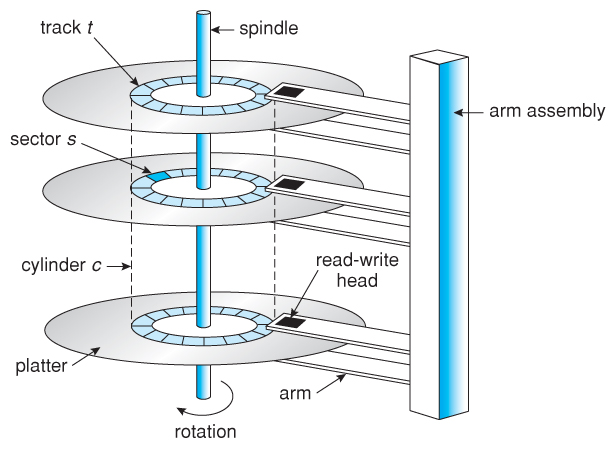
\includegraphics[scale=0.8]{./Drawings/EDAF35-Operating_Systems/Magnetic_Disk_Mechanism.jpg}
  \caption{Magnetic Disk Moving head Mechanism}
  \label{fig:HDD_Mechanism}
\end{figure}

When the disk is in use, a drive motor spins it at high speed.
Common drives spin at \SIlist{5400; 7200; 10000; 15000}{\rpm}.
Disk speed has two parts.
\begin{enumerate}[noitemsep]
\item The transfer rate is the rate at which data flow between the drive and the computer.
\item The positioning time, or random-access time. Itself consisting of 2 parts:
  \begin{enumerate}[noitemsep]
  \item Time necessary to move the disk arm to the desired cylinder, called the seek time,
  \item Time necessary for the desired sector to rotate to the disk head, called the rotational latency.
  \end{enumerate}
\end{enumerate}


%%% Local Variables:
%%% mode: latex
%%% TeX-master: "../../EDAF35-Operating_Systems-Reference_Sheet"
%%% End:


\subsection{Disk Structure}\label{subsec:Disk_Structure}
Here, we view all potential storage media (\Cref{subsec:Structure_Storage_Media}) as being the same.

Drives are addressed as large one-dimensional arrays of \nameref{def:Logical_Block}s.


%%% Local Variables:
%%% mode: latex
%%% TeX-master: "../../EDAF35-Operating_Systems-Reference_Sheet"
%%% End:


\subsection{Disk Attachment}\label{subsec:Disk_Attachment}
This section is concerned with how these physical disks or tapes are attached to the computer for use.
There are 2 ways to access disk storage:
\begin{enumerate}[noitemsep]
\item \nameref{def:Host_Attached_Storage}
\item \nameref{def:Network_Attached_Storage}
\end{enumerate}

\subsubsection{Host-Attached Storage}\label{subsubsec:Host_Attached_Storage}
In \nameref{def:Host_Attached_Storage} any combination of I/O bus architectures and protocols can be used.
The I/O commands that initiate data transfers to a host-attached storage device are reads and writes of logical data blocks directed to specifically identified storage units (such as bus ID or target logical unit).


%%% Local Variables:
%%% mode: latex
%%% TeX-master: "../../EDAF35-Operating_Systems-Reference_Sheet"
%%% End:


\subsection{Disk Scheduling}\label{subsec:Disk_Scheduling}
Just like with CPU~\nameref{subsec:Scheduling} and \nameref{sec:Virtual_Memory}, the \nameref{def:Operating_System} attempts to maximize the efficient use of hardware resources.
For disk drives, this means minimizing access time and maximizing bandwidth.

\begin{definition}[Disk Bandwidth]\label{def:Disk_Bandwidth}
  The \emph{disk bandwidth} is the total number of bytes transferred, divided by the total time between the first request for service and the completion of the last transfer.

  The service time will include the seek time (time for disk arm to move heads to cylinder) and the rotational latency (time for platter to spin to correct sector).
\end{definition}

When performing disk I/O, we need to know a few things:
\begin{itemize}[noitemsep]
\item Whether this operation is input or output.
\item What the disk address for the transfer is.
\item What the memory address for the transfer is.
\item What the number of sectors to be transferred is.
\end{itemize}

If the desired disk drive \textbf{and} controller are available, the request can be serviced immediately.
If the drive or controller is busy, any new requests for service will be placed in the queue of pending requests for that drive.

Like before, the choice of how to handle pending requests in the queue is handled by the choice of disk-scheduling algorithm.
Choosing the best one is difficult because performance depends heavily on the number and types of requests.
\nameref{subsubsec:SSTF_Disk_Scheduling} is common and has a natural appeal because it increases performance over \nameref{subsubsec:FCFS_Disk_Scheduling}.
\nameref{subsubsec:SCAN_Disk_Scheduling} and \nameref{par:Circular_SCAN_Disk_Scheduling} perform better for systems that place a heavy load on the disk, because they are less likely to cause a starvation problem.
For any particular list of requests, we \textbf{can} define an optimal order of retrieval, but the computation needed to find an optimal schedule may not justify the savings over SSTF or SCAN.\@
Because of the complexity involved with this topic, and the potential cost by choosing the wrong algorithm, the disk-scheduling algorithm should be a separate module of the OS, so it can be replaced if need be.

Requests for disk service can be greatly influenced by the file-allocation method.
A program reading a contiguously allocated file will generate several requests that are close together on the disk, resulting in limited head movement.
A linked or indexed file, in contrast, may include blocks that are widely scattered on the disk, resulting in greater head movement.
The location of directories and index blocks is also important.
Since every file must be opened to be used, and opening a file requires searching the directory structure, the directories will be accessed frequently.

\subsubsection{First-Come First-Serve Scheduling}\label{subsubsec:FCFS_Disk_Scheduling}
This version of \emph{First-Come First-Serve Scheduling} is like all the others discussed earlier.
The first disk seek request that comes into the queue is handled first, without regard to the distance the head must travel to find the requested data.

\subsubsection{Shortest-Seek-Time-First Scheduling}\label{subsubsec:SSTF_Disk_Scheduling}
\emph{Shortest-Seek-Time-First Scheduling} services all the requests close to the current head position before moving the head far away to service other requests.
This method selects the request with the least seek time from the current head position.


%%% Local Variables:
%%% mode: latex
%%% TeX-master: "../../EDAF35-Operating_Systems-Reference_Sheet"
%%% End:


\subsection{Disk Management}\label{subsec:Disk_Management}

%%% Local Variables:
%%% mode: latex
%%% TeX-master: "../../EDAF35-Operating_Systems-Reference_Sheet"
%%% End:


%%% Local Variables:
%%% mode: latex
%%% TeX-master: "../EDAF35-Operating_Systems-Reference_Sheet"
%%% End:


\section{File-System Interface}\label{sec:FS_Interface}
So that the computer system will be convenient to use, the \nameref{def:Operating_System} provides a uniform logical view of stored information, the \nameref{def:File}.

\defFile{}

Files in all \nameref{def:Operating_System}s have attributes that help describe them.
\begin{itemize}[noitemsep]
\item \textbf{Name}.
  The symbolic file name is the only information kept in human-readable form.
\item \textbf{Identifier}.
  This unique tag, usually a number, identifies the file within the file system; it is the non-human-readable name for the file.
\item \textbf{Type}.
  This information is needed for systems that support different types of files.
\item \textbf{Location}.
  This information is a pointer to a device and to the location of the file on that device.
\item \textbf{Size}.
  The current size of the file and possibly the maximum allowed size are included in this attribute.
\item \textbf{Protection}.
  Access-control information determines who can do reading, writing, executing, etc.
\item \textbf{Time, date, and user identification}.
  This information may be kept for creation, last modification, and last use.
  This data can be useful for protection, security, and usage monitoring.
\end{itemize}

The information about all files is kept in the directory structure, which is also on secondary storage.
An entry in a directory consists of the file’s name and its unique identifier.
The file's identifier in turn locates the other file attributes.
It may take more than a kilobyte to record this information for each file.
Because directories must also be nonvolatile, they must be stored on the device and brought into memory as needed.

\subsection{File Operations}\label{subsec:File_Operations}
A file is an abstract data type, as such, to define a file properly, we need to consider the operations that can be performed on files.


%%% Local Variables:
%%% mode: latex
%%% TeX-master: "../../EDAF35-Operating_Systems-Reference_Sheet"
%%% End:


\subsection{File Types}\label{subsec:File_Types}
We need to decide whether the operating system should recognize and support \nameref{def:File} types.
If an operating system recognizes the type of a file, it can then operate on the file in reasonable ways.


%%% Local Variables:
%%% mode: latex
%%% TeX-master: "../../EDAF35-Operating_Systems-Reference_Sheet"
%%% End:


\subsection{File Structure}\label{subsec:File_Structure}
File types can also indicate the internal structure of the file.
This point brings us to one of the disadvantages of having the operating system support multiple file structures: the resulting size of the operating system is cumbersome.
If the operating system defines five different file structures, it needs to contain the code to support these file structures.

Some operating systems impose (and support) a minimal number of file structures.
\textsc{unix} considers each file to be a sequence of bytes; no interpretation of these bits is made by the \textbf{\nameref{def:Operating_System}}.
Each application program must include its own code to interpret an input file as to the appropriate structure.
This scheme provides maximum flexibility but little support.
All operating systems must support at least one structure, the executable file, so that the system is able to load and run programs.


%%% Local Variables:
%%% mode: latex
%%% TeX-master: "../../EDAF35-Operating_Systems-Reference_Sheet"
%%% End:


\subsection{Access Methods}\label{subsec:Access_Methods}
\nameref{def:File}s store information.
When they are used, this information must be accessed and read into computer memory.
The 2 main ways to access the content of a file are:
\begin{enumerate}[noitemsep]
\item \nameref{subsubsec:Sequential_Access}
\item \nameref{subsubsec:Direct_Access}
\end{enumerate}

Not all operating systems support both \nameref{subsubsec:Sequential_Access} and \nameref{subsubsec:Direct_Access} for files.
Some systems allow only sequential file access; others allow only direct access.
Some systems require that a file be defined as sequential or direct when it is created.
Such a file can be accessed only in a manner consistent with its declaration.

\subsubsection{Sequential Access}\label{subsubsec:Sequential_Access}
Information in the file is processed in order, one logical record after the other.
This mode of access is by far the most common.

Reads and writes make up the bulk of the operations on a file.
A read operation reads the next portion of the file and automatically advances a file pointer, tracking the I/O location.
Similarly, the write operation, appends to the end of the file and advances to the end of the newly written material (the new end of file).

The pointers in this file can be reset to the beginning, and on some systems, a program may be able to skip forward or backward $n$ records for some integer $n$—perhaps only for $n = 1$.
Sequential access is based on a tape model of a file and works as well on sequential-access devices as it does on random-access ones.


%%% Local Variables:
%%% mode: latex
%%% TeX-master: "../../EDAF35-Operating_Systems-Reference_Sheet"
%%% End:


\subsection{Directory and Disk Structure}\label{subsec:Directory_Disk_Structure}
Each \nameref{def:Volume} that contains a \nameref{def:File_System} must also contain information about the \nameref{def:File}s in the system.
This information is kept in entries in a device directory (A volume's Table of Contents).
The device directory (commonly, the \nameref{def:Directory}) records information—such as name, location, size, and type—for all files on that volume.

\begin{definition}[Volume]\label{def:Volume}
  A \emph{Volume} is a logical view of the installed disks.
  Any entity that contains a \nameref{def:File_System} is considered a volume.
  In the case of a \nameref{def:RAID} setup, when members are pooled together, they are collectively addressed as a single volume.
\end{definition}

\subsubsection{Storage Structure}\label{subsubsec:Storage_Structure}
A general-purpose computer system has multiple storage devices, and those devices can be sliced up into \nameref{def:Volume}s that hold \nameref{def:File_System}s.
Computer systems may have zero or more file systems, and the file systems may be of varying types.

The file systems of computers can be extensive.
Even within a file system, it is useful to segregate files into groups and manage and act on those groups.
This organization involves the use of directories.

\subsubsection{Directory Overview}\label{subsubsec:Directory_Overview}
\begin{definition}[Directory]\label{def:Directory}
  The directory can be viewed as a symbol table that translates file names into their directory entries.
  Directories are files that are responsible for tracking and holding other files, which themselves may be directories.
\end{definition}

The directory itself can be organized in many ways.
The organization must allow us to insert entries, to delete entries, to search for a named entry, and to list all the entries in the directory.

Like a \nameref{def:File}, a \nameref{def:Directory} can be seen as an abstract data type that needs its computations defined before being concrete.
\begin{itemize}[noitemsep]
\item \textbf{Search for a file}.
  We need to be able to search a directory structure to find the entry for a particular file.
  Since files have symbolic names, and similar names may indicate a relationship among files, we may want to be able to find all files whose names match a particular pattern.

\item \textbf{Create a file}.
  New files need to be created and added to the directory.

\item \textbf{Delete a file}.
  When a file is no longer needed, we want to be able to remove it from the directory.

\item \textbf{List a directory}.
  We need to be able to list the files in a directory and the contents of the directory entry for each file in the list.

\item \textbf{Rename a file}.
  Because the name of a file represents its contents to its users, we must be able to change the name when the contents or use of the file changes.
  Renaming a file may also allow its position within the directory structure to be changed.

\item \textbf{Traverse the file system}.
  We may wish to access every directory and every file within a directory structure.
  For reliability, it is a good idea to backup the contents and structure of the entire file system at regular intervals.
\end{itemize}

\subsubsection{Single-Level Directory}\label{subsubsec:Single_Level_Directory}
All files are contained in the same directory, which is easy to support and understand.

However, there are significant limitations.
\begin{itemize}[noitemsep]
\item When the number of files increases or when the system has more than one user.
\item Since all files are in the same directory, they must have unique names.
\item If two users call their data file the same thing, then the unique-name rule is violated.
\end{itemize}

\subsubsection{Two-Level Directory}\label{subsubsec:Two_Level_Directory}
The standard solution is to create a separate directory for each user.
In the two-level directory structure, each user has their own User File Directory (UFD).
The UFDs have similar structures, but each lists only the files of a \textbf{single} user.
When a user job starts or a user logs in, the system’s Master File Directory (MFD) is searched for that user's UFD.\@
The MFD is indexed by user name or account number, and each entry points to the UFD for that user.

\begin{itemize}[noitemsep]
\item When a user refers to a particular file, only their own UFD is searched.
  Allowing different users to have files with the same name, as long as all the file names within each UFD are unique.
\item To create a file for a user, the operating system searches only that user’s UFD to ascertain whether another file of that name exists.
\item To delete a file, the operating system confines its search to the local UFD.\@
  Preventing the accidental deletion of another user’s file that has the same name.
\end{itemize}

The user directories themselves must be created and deleted as necessary.
A special system program can be run with the appropriate user name and account information.
The program creates a new UFD and adds an entry for it to the MFD.\@

However, this structure effectively isolates one user from another.
Isolation is a disadvantage when the users want to cooperate on some task and to access one another's files.
Some systems simply do not allow local user files to be accessed by other users, requiring a dedicated shared space.
If access is to be permitted, one user must have the ability to name a file in another user’s directory.
To name a particular file uniquely in a two-level directory, we must give both the user name and the file name.

\begin{definition}[Path Name]\label{def:Path_Name}
  A \emph{path name} is the list of directories and their names that must traversed before finally arriving at a file.
  Every file \textbf{MUST} have a path name to be identified.
  Note that there is no requirement for every file to have a \textbf{UNIQUE} path name.

  For example, \url{/etc/fstab} on \textsc{unix}-based machines.

  There are Absolute Path Names and Relative Path Names.
  An absolute path name begins at the root and follows a path down to the specified file, giving the directory names on the path.
  A relative path name defines a path from the current directory.

  \begin{remark}[Path Names with Volumes]
    Additional syntax is needed to specify the \nameref{def:Volume} of a file.
  \end{remark}
\end{definition}

A special instance of this situation occurs with the shared system files.
Programs provided as part of the system (loaders, assemblers, compilers, utility routines, libraries, etc.) are generally defined as \nameref{def:File}s.
When the appropriate commands are given, these files are read by the loader and executed.
Many command interpreters simply treat such a command as the name of a file to load and execute.

The standard solution is to complicate the search procedure slightly.
A special user directory is defined to contain the system files.
Whenever a file name is given to be loaded, the operating system first searches the local UFD.\@
If the file is found, it is used.
If it is not found, the system automatically searches the special user directory that contains the system files.

\begin{definition}[Search Path]\label{def:Search_Path}
  The sequence of directories searched when a file is named is called the \emph{search path}.
  The search path can be extended to contain an unlimited list of directories to search when a command name is given.
  Systems can also be designed so that each user has their own search path.
\end{definition}

\subsubsection{Tree-Structured Directory}\label{subsubsec:Tree_Structured_Directory}
The natural generalization of the \nameref{subsubsec:Two_Level_Directory} is to extend the directory structure to a tree of arbitrary height.
This generalization allows users to create their own subdirectories and to organize their files accordingly.
The tree has a root directory, and every file in the system has a unique \nameref{def:Path_Name}.

A directory contains a set of files and/or subdirectories.
A directory is another file, but treated in a special way.
All directories have the same internal format.
One bit in each directory entry defines the entry as a file (0) or as a subdirectory (1), a crude magic number.
Special \nameref{def:System_Call}s are used to create and delete directories.

In normal use, each process has a current directory.
The current directory should contain most of the files that are of current interest to the process.
When reference is made to a file, the current directory is searched.
If a file is needed that is not in the current directory, then the user usually must either specify a path name or change the current directory to be the directory holding that file.

The initial current directory of a user’s login shell is designated when the user job starts or the user logs in.
The operating system searches the accounting file to find an entry for this user.
In the accounting file is a pointer to (or the name of) the user’s initial directory.
This pointer is copied to a local variable for this user that specifies the user’s initial current directory.
From there, other processes can be spawned.
The current directory of any subprocess is usually the current directory of the parent when it was spawned.

An interesting decision in this setup how to delete a directory.
\begin{itemize}[noitemsep]
\item If a directory is empty, its entry in the
  directory that contains it can simply be deleted.
\item If the directory is not empty (Some systems will not delete a directory unless it is empty), one of two approaches can be taken.
  \begin{enumerate}[noitemsep]
  \item the user must first delete all the files in that directory.
    If any subdirectories exist, this procedure must be applied recursively to them, so that they can be deleted also.
    This approach can result in a substantial amount of work.
  \item An alternative, such as that taken by the \textsc{unix} \texttt{rm} command, is to use an option.
    When a request is made to delete a directory, all that directory’s files and subdirectories are also to be deleted.
  \end{enumerate}
\end{itemize}

With a tree-structured directory system, users can be allowed to access the files of other users.
This can be done with either an absolute or a relative \nameref{def:Path_Name}.
It could also be done with one user changing their current directory.


%%% Local Variables:
%%% mode: latex
%%% TeX-master: "../../EDAF35-Operating_Systems-Reference_Sheet"
%%% End:


\subsection{File System Mounting}\label{subsec:File_System_Mounting}
Just as a \nameref{def:File} must be opened before it is used, a \nameref{def:File_System} must be mounted before it can be available to \nameref{def:Process}es on the system.
Specifically, the directory structure may be built out of multiple \nameref{def:Volume}s, which must be mounted to make them available within the file-system name space.


%%% Local Variables:
%%% mode: latex
%%% TeX-master: "../../EDAF35-Operating_Systems-Reference_Sheet"
%%% End:


\subsection{File Sharing}\label{subsec:File_Sharing}
File sharing is very desirable for users who want to collaborate and to reduce the effort required to achieve a computing goal.
Therefore, user-oriented operating systems must accommodate the need to share files in spite of the inherent difficulties.

\subsubsection{Multiple Users}\label{subsubsec:File_Sharing-Multiple_Users}
Given a directory structure that allows files to be shared by users, the system must mediate the file sharing.
The system can either allow a user to access the files of other users by default or require that a user specifically grant access to the files.
To implement sharing and protection, the system must maintain more file and directory attributes than are needed on a single-user system.
Typically, this involves recording the \nameref{def:File_Owner} and the \nameref{def:File_Group} to determine access.

This is discussed more in \Cref{subsec:File_Protection}.

\subsubsection{Remote File Systems}\label{subsubsec:Remote_File_Systems}
With the advent of networks, communication among remote computers became possible.
Networking allows the sharing of resources spread over a distance.
One obvious resource to share is data in the form of files.

There are 2 main methods for transferring files between computing systems.
\begin{enumerate}[noitemsep]
\item Manual programs, like \texttt{ftp}. The World Wide Web falls into this category too.
\item \nameref{def:Distributed_File_System}s. There are 2 main models and 1 main concern.
  \begin{enumerate}[noitemsep]
  \item \nameref{par:Client_Server_Model}.
  \item \nameref{par:Distributed_Information_Systems}.
  \end{enumerate}
  \begin{enumerate}[noitemsep]
  \item \nameref{par:Failure_Modes}.
  \end{enumerate}
\end{enumerate}

\begin{definition}[Distributed File System]\label{def:Distributed_File_System}
  A \emph{Distributed File System} (\emph{DFS}) is where remote directories are visible from a local machine, as if the file storage were directly attached to the computer.
\end{definition}

\paragraph{Client-Server Model}\label{par:Client_Server_Model}
The machine containing the files is the server, and the machine seeking access to the files is the client.
Generally, the server declares that a resource is available to clients and specifies exactly which resource and exactly which clients.
A server can serve multiple clients, and a client can use multiple servers, depending on the implementation details of a given client–server facility.

Client identification is more difficult.
A client can be specified by a network name or other identifier, such as an IP address, but these can be spoofed.
More secure solutions include secure authentication of the client via encrypted keys.
Unfortunately, with security come many challenges, including ensuring compatibility of the client and server and security of key exchanges.

\paragraph{Distributed Information Systems}\label{par:Distributed_Information_Systems}
Distributed information systems, also known as distributed naming services, provide unified access to the information needed for remote computing.
The Domain Name System (DNS) is one example of this type of information system.

Other distributed information systems provide user name/password/user ID/group ID space for a distributed facility.
This allows all computer-related information to be tracked and stored in a single central place and information be shared out on an as-needed basis.

\paragraph{Failure Modes}\label{par:Failure_Modes}
Local file systems can fail for a variety of reasons, including:
\begin{itemize}[noitemsep]
\item Failure of the disk containing the file system.
\item Corruption of the directory structure or other disk-management information (collectively called metadata).
\item Disk-controller failure.
\item Cable failure.
\item Host-adapter failure.
\item User failure can also cause files to be lost or entire directories or volumes to be deleted.
\item System-Administrator can cause files to be lost or entire directories or volumes to be deleted.
\end{itemize}

Many of these failures will cause a host to crash and an error condition to be displayed, and human intervention will be required to repair the damage.

Remote file systems have even more failure modes.
Because of the complexity of network systems and the required interactions between remote machines, many more problems can interfere with the proper operation of remote file systems.

For example, what would happen if the remote file system became no longer reachable?
This scenario is rather common, so it would not be appropriate for the client system to act as it would if a local file system were lost.
Instead, the system can either terminate all operations to the lost server or delay operations until the server is again reachable.

\subsubsection{Consistency Semantics}\label{subsubsec:Consistency_Semantics}
Consistency semantics represent an important criterion for evaluating any file system that supports file sharing.
These semantics specify how multiple users of a system are to access a shared file simultaneously.

Consistency semantics are directly related to \nameref{def:Process} \nameref{subsec:Synchronization} algorithms.
However, those complex algorithms tend not to be implemented in the case of file I/O because of the great latencies and slow transfer rates of disks and networks.

For the following discussion, we assume that a series of file accesses attempted by a user to the same file is always enclosed between the \kernelinline{open()} and \kernelinline{close()} operations.
The accesses between the \kernelinline{open()} and \kernelinline{close()} operations makes up a file session.

\paragraph{\textsc{unix} Semantics}\label{par:UNIX_Consistency_Semantics}
\textsc{unix} uses the following consistency semantics:
\begin{itemize}[noitemsep]
\item Writes to an open file by a user are visible immediately to other users who have this file open.
\item \textsc{unix} had a mode of sharing that allows users to share the pointer of current location into the file.
  Thus, the advancing of the pointer by one user affects all sharing users.
  Here, a file has a single image that interleaves all accesses, regardless of their origin.
\end{itemize}


%%% Local Variables:
%%% mode: latex
%%% TeX-master: "../../EDAF35-Operating_Systems-Reference_Sheet"
%%% End:


\subsection{Protection}\label{subsec:File_Protection}
When information is stored in a computer system, we want to keep it safe from improper access.

Most systems have evolved to use the concepts of file \nameref{def:File_Owner} and \nameref{def:File_Group}.

\subsubsection{Types of Access}\label{subsubsec:Types_File_Access}
The need to protect files is a direct result of the ability to access files.
Systems that do not permit access to the files of other users do not need protection.
Protection mechanisms provide controlled access by limiting the types of file access that can be made.
Access is permitted or denied depending on several factors, one of which is the type of access requested.
Several different types of operations may be controlled:
\begin{itemize}[noitemsep]
\item \textbf{Read}.
 Read from the file.
\item \textbf{Write}.
 Write or rewrite the file.
\item \textbf{Execute}.
 Load the file into memory and execute it.
\item \textbf{Append}.
 Write new information at the end of the file.
\item \textbf{Delete}.
 Delete the file and free its space for possible reuse.
\item \textbf{List}.
 List the name and attributes of the file.
\end{itemize}


%%% Local Variables:
%%% mode: latex
%%% TeX-master: "../../EDAF35-Operating_Systems-Reference_Sheet"
%%% End:


%%% Local Variables:
%%% mode: latex
%%% TeX-master: "../EDAF35-Operating_Systems-Reference_Sheet"
%%% End:


\section{File-System Implementation}\label{sec:FS_Implementation}

%%% Local Variables:
%%% mode: latex
%%% TeX-master: "../EDAF35-Operating_Systems-Reference_Sheet"
%%% End:


\section{I/O Systems}\label{sec:IO_Systems}
Because I/O devices vary so widely in their function and speed, varied methods are needed to control them.
These methods form the I/O subsystem of the kernel, which separates the rest of the kernel from the complexities of managing I/O devices.

To encapsulate the details and oddities of different devices, the kernel of an operating system is structured to use \nameref{def:Device_Driver} modules.

\begin{definition}[Device Driver]\label{def:Device_Driver}
  \emph{Device Driver}s present a uniform device-access interface to the I/O subsystem.
  Every device requires a device driver (though certain devices can reuse another device's driver).
  The device driver hides the device-specific implementation details from the \nameref{def:Operating_System} and I/O subsystem, and only showing a standard, uniform interface.
  The type of interface exported depends on the nature of the device itself.

  This is analogous to \nameref{def:System_Call}s providing a standard interface between the application and the \nameref{def:Operating_System}.
\end{definition}

Despite the incredible variety of I/O devices, though, we need only a few concepts to understand how the devices are attached and how the software can control the hardware.

\subsection{I/O Hardware}\label{subsec:IO_Hardware}
The device communicates with the machine via a connection point, a port.
If devices share a common set of wires, the connection is called a \nameref{def:Hardware_Bus}.
Buses are used widely in computer architecture and vary in their signaling methods, speed, throughput, and connection methods.

\begin{definition}[Bus]\label{def:Hardware_Bus}
  A \emph{bus} is a set of wires and a rigidly defined protocol that specifies a set of messages that can be sent on the wires.
\end{definition}

When device A plugs into device B, and device B plugs into device C, and device C plugs into a port on the computer, this arrangement is called a daisy chain.
A daisy chain usually operates as a \nameref{def:Hardware_Bus}.

All of these may be controlled by a \nameref{def:Controller}.

\begin{definition}[Controller]\label{def:Controller}
  A \emph{controller} is a collection of electronics that can operate a port, a \nameref{def:Hardware_Bus}, or a device.
\end{definition}

Because some protocols are complex, their \nameref{def:Hardware_Bus} \nameref{def:Controller} is often implemented as a separate circuit board (or a host adapter) that plugs into the computer.
It typically contains a processor, microcode, and some private memory to enable it to process the protocol messages.
Some devices have their own built-in controllers.
They can receive commands in 2 ways (some support both, some do not):
\begin{enumerate}[noitemsep]
\item The \nameref{def:Controller} has one or more registers for data and control signals.
  The processor communicates with the controller by reading and writing bit patterns in these registers.
  This communication can occur through the use of special I/O instructions that specify the transfer of a byte or word to an I/O port address.
  The I/O instruction triggers bus lines to select the proper device and to move bits into or out of a device register.
\item The device \nameref{def:Controller} can support \nameref{subsubsec:Memory_Mapped_IO}.
  In this case, the device-control registers are mapped into the address space of the processor.
  The CPU executes I/O requests using the standard data-transfer instructions to read and write the device-control registers at their mapped locations in physical memory.
\end{enumerate}

For example, a graphics controller supports both of these methods of control.
\begin{itemize}[noitemsep]
\item The graphics controller has I/O ports for basic control operations.
\item The controller has a large memory-mapped region to hold screen contents.
  The process sends output to the screen by writing data into the memory-mapped region.
  The controller generates the screen image based on the contents of this memory.
\end{itemize}

The ease of writing to a \nameref{subsubsec:Memory_Mapped_IO} \nameref{def:Controller} is offset by the disadvantage of being vulnerable to accidental modification by an incorrect pointer to an unintended region of memory.
Memory protection helps reduce this risk.

\subsubsection{I/O Ports}\label{subsubsec:IO_Ports}
An I/O port typically consists of four registers, called the status, control, data-in, and data-out registers.
\begin{enumerate}[noitemsep]
\item The \textbf{\texttt{data-in} register} is read by the host to get input.
\item The \textbf{\texttt{data-out} register} is written by the host to send output.
\item The \textbf{\texttt{status} register} contains bits that can be \textbf{read by the host}.
  These bits indicate states, such as:
  \begin{itemize}[noitemsep]
  \item Whether the current command has completed.
  \item Whether a byte is available to be read from the data-in register.
  \item Whether a device error has occurred.
  \end{itemize}

\item The \textbf{\texttt{control} register} can be \textbf{written by the host} to start a command or to change the mode of a device.
  For instance:
  \begin{itemize}[noitemsep]
  \item One bit in a register of a serial port chooses between full-duplex and half-duplex communication.
  \item Another bit enables parity checking.
  \item A third bit sets the word length to different bit lengths.
  \item Other bits select one of the speeds supported by the serial port.
  \end{itemize}
\end{enumerate}

\subsubsection{Polling}\label{subsubsec:Polling}
The controller indicates its state through the \texttt{busy} bit in the \texttt{status} register.
The controller sets the \texttt{busy} bit when it is busy working and clears it when the controller is ready to accept the next command.
The host signals its wishes by setting the \texttt{command-ready} bit in the \texttt{command} register when a command is available for the controller to execute.

The repeating loop of polling is described in the following steps:
\begin{enumerate}[noitemsep]
\item The host repeatedly reads the \texttt{busy} bit until that bit becomes clear.
\item The host sets the \texttt{write} bit in the \texttt{command} register and writes a byte into the \texttt{data-out} register.
\item The host sets the \texttt{command-ready} bit.
\item When the controller notices that the \texttt{command-ready} bit is set, it sets the busy bit.
\item The controller reads the \texttt{command} register and sees the \texttt{write} command.
  It reads the \texttt{data-out} register to get the byte and does the I/O to the device.
\item The controller clears the \texttt{command-ready} bit, clears the error bit in the status register to indicate that the device I/O succeeded, and clears the \texttt{busy} bit to indicate that it is finished.
\end{enumerate}

The host is \textbf{busy-waiting} or \textbf{polling} in the first step: it is in a loop, reading the status register over and over until the busy bit becomes clear.
If the controller and device are fast, this is reasonable.
But if the wait is long enough, the host should switch to another task.

For some devices, the host \textbf{must} service the device quickly, or data will be lost.
For instance, when data are streaming in on a serial port, the small buffer on the controller will overflow and data will be lost if the host waits too long before returning to read the bytes.

The basic polling operation is instruction-efficient.
In many computer architectures, just three CPU-instruction cycles are sufficient to poll a device:
\begin{enumerate}[noitemsep]
\item Read a device register.
\item Logical \texttt{AND} to extract a status bit.
\item Branch if not zero.
\end{enumerate}

But polling becomes inefficient when it is attempted repeatedly yet rarely finds a device ready for service, while other useful CPU processing remains undone.
In those cases, it is more efficient to have the hardware controller notify the CPU when the device becomes ready again, rather than require the CPU to poll for I/O completion.
The hardware mechanism that enables a device to notify the CPU is called an \nameref{def:Interrupt}.

\subsubsection{Interrupts}\label{subsubsec:Interrupts}
The CPU hardware has a wire called the \nameref{def:Interrupt_Request_Line} that the CPU senses after executing every instruction.

\begin{definition}[Interrupt-Request Line]\label{def:Interrupt_Request_Line}
  The \emph{interrupt-request line} is a dedicated hardware line or \nameref{def:Hardware_Bus} for sending information about exceptional circumstances to the CPU.\@
  The CPU checks this line after \textbf{every} instruction.

  If the line does not contain any information, the CPU continues normal execution.
  If it does contain some information, then the CPU performs a \nameref{def:Context_Switch}.
  However, instead of switching to another \nameref{def:Process}, the CPU jumps to the \nameref{def:Interrupt_Handler}.
\end{definition}

When the CPU detects that a controller has asserted a signal on the interrupt-request line, the CPU performs a state save and jumps to the \nameref{def:Interrupt_Handler} routine at a fixed address in memory.

\begin{definition}[Interrupt Handler]\label{def:Interrupt_Handler}
  The \emph{interrupt handler}:
  \begin{enumerate}[noitemsep]
  \item Determines the cause of the interrupt.
  \item Performs the necessary processing.
  \item Performs a state restore.
  \item Executes a return from interrupt instruction to return the CPU to the execution state prior to the interrupt.
  \end{enumerate}
\end{definition}

The basic loop of an \nameref{def:Interrupt}-driven \nameref{def:Operating_System} is:
\begin{enumerate}[noitemsep]
\item The device controller \textbf{raises} an interrupt by asserting a signal on the \nameref{def:Interrupt_Request_Line}.
\item The CPU \textbf{catches} the interrupt and \textbf{dispatches} it to the \nameref{def:Interrupt_Handler}.
\item The handler \textbf{clears} the interrupt by servicing the device.
\item The CPU returns to normal execution.
\end{enumerate}


%%% Local Variables:
%%% mode: latex
%%% TeX-master: "../../EDAF35-Operating_Systems-Reference_Sheet"
%%% End:


\subsection{Application I/O Interface}\label{subsec:Application_IO_Interface}
The \nameref{def:Operating_System} wants to treat all I/O devices in a standard, uniform way.
Like other complex software-engineering problems, the approach here involves abstraction, encapsulation, and software layering.
Specifically, we can abstract away the detailed differences in I/O devices by identifying a few general kinds, where each is accessed through a standardized set of functions, its \emph{interface}.
The implementation differences are encapsulated in \nameref{def:Kernel_Module}s called \nameref{def:Device_Driver}s that internally are custom-tailored to specific devices but that export one of the standard interfaces.
The software layering used is shown in \Cref{fig:Kernel_IO_Subsystem_Structure}.

\begin{figure}[h!tbp]
  \centering
  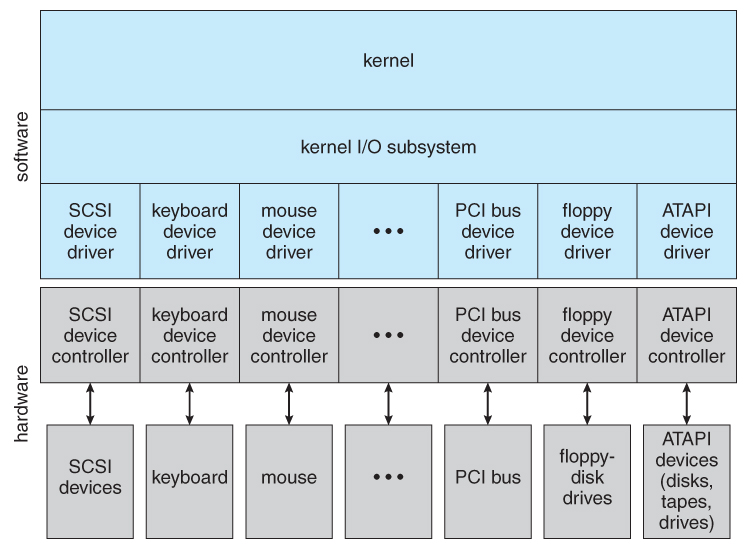
\includegraphics[scale=1.00]{./Drawings/EDAF35-Operating_Systems/Kernel_IO_Subsystem_Structure.jpg}
  \caption{Kernel I/O Subsystem Structure}
  \label{fig:Kernel_IO_Subsystem_Structure}
\end{figure}

This layering methodology is used to hide differences among devices and their controllers from the \nameref{def:Kernel}'s I/O subsystem.
This is analogous to the I/O system calls encapsulating the behavior of devices in a few generic classes that hide hardware differences from applications.

Making the I/O subsystem independent of the hardware simplifies the job of the operating-system developer.
It also benefits the hardware manufacturers.
They either:
\begin{itemize}[noitemsep]
\item Design new devices to be compatible with an existing host controller interface.
\item Write device drivers to interface the new hardware to popular operating systems.
\end{itemize}

Thus, we (users) can attach new peripherals to a computer without waiting for the operating system to develop explicit kernel-level support code.
Unfortunately for hardware manufacturers, each operating system has its own standards for the device-driver interface.

Devices can vary in many dimensions, as seen in \Cref{tab:Characteristics_IO_Devices}.
\begin{table}[h!tbp]
  \centering
  \begin{tabular}{cll}
    \toprule
    \textbf{Aspect} & \textbf{Variation} & \textbf{Example} \\
    \midrule
    \multirow{2}{*}{Data-Transfer Mode} & Character & Terminal \\
                    & Block & Disk \\
    \multirow{2}{*}{Access Method} & Sequential & Modem/Network \\
                    & Random & Magnetic Disk \\
    \multirow{2}{*}{Transfer Schedule} & Synchronous & Magnetic Tape \\
                    & Asynchronous & Keyboard \\
    \multirow{2}{*}{Sharing} & Dedicated & Magnetic Tape \\
                    & Sharable & Keyboard \\
    \multirow{4}{*}{Device Speed} & Latency & \\
                    & Seek Time & \\
                    & Transfer Rate & \\
                    & Delay between Operations & \\
    \multirow{3}{*}{I/O Direction} & & \\
                    & Read-only & CD-ROM (After first write) \\
                    & Write-only & Graphics Controller \\
                    & Read-write & Disk \\
    \bottomrule
  \end{tabular}
  \caption{Characteristics of I/O Devices}
  \label{tab:Characteristics_IO_Devices}
\end{table}

%%% Local Variables:
%%% mode: latex
%%% TeX-master: "../../EDAF35-Operating_Systems-Reference_Sheet"
%%% End:


\subsection{Kernel I/O Subsystem}\label{subsec:Kernel_IO_Subsystem}
Kernels provide many services related to I/O, which build on the hardware and \nameref{def:Device_Driver} infrastructure, including:
\begin{itemize}[noitemsep]
\item \nameref{subsubsec:IO_Scheduling}.
\item \nameref{subsubsec:IO_Buffering}.
\item \nameref{subsubsec:IO_Caching}.
\item \nameref{subsubsec:Spooling_Device_Reservation}.
\item \nameref{subsubsec:IO_Error_Handling}.
\end{itemize}

The I/O subsystem is also responsible for protecting itself from errant processes and malicious users.

\subsubsection{I/O Scheduling}\label{subsubsec:IO_Scheduling}
To schedule a set of I/O requests means to determine a good order in which to execute them.
The order in which applications issue system calls rarely is the best choice.
Scheduling can improve overall system performance, can share device access fairly among processes, and can reduce the average waiting time for I/O to complete.

Operating-system developers implement scheduling by maintaining a queue of requests for each device.
When an application issues a \nameref{def:Blocking_Syscall} I/O system call, the request is placed on the queue for \textbf{that} device.
The I/O scheduler rearranges the order of the queue to improve the overall system efficiency and the average response time experienced by applications.
The operating system may also try to be fair, so that no one application receives especially poor service, or it may give priority service for delay-sensitive requests.

When a kernel supports \textbf{asynchronous} I/O, it must be able to keep track of many I/O requests at the same time.
For this purpose, the operating system might attach the wait queue to a device-status table.
The kernel manages this table, which contains an entry for each I/O device.
Each entry indicates:
\begin{itemize}[noitemsep]
\item The device's type
\item Address
\item State (not functioning, idle, or busy)
  \begin{itemize}[noitemsep]
  \item If the device is busy with a request, the type of request and other parameters will be stored in the table entry for that device.
  \end{itemize}
\end{itemize}

\subsubsection{Buffering}\label{subsubsec:IO_Buffering}
Buffering is done for three reasons.
\begin{enumerate}[noitemsep]
\item One reason is to cope with a speed mismatch between the producer and consumer of a data stream.
\item A second use of buffering is to provide adaptations for devices that have different data-transfer sizes.
\item A third use of buffering is to support copy semantics for application I/O.
  \begin{itemize}[noitemsep]
  \item Copy semantics are such that writing to a disk will not corrupt any data.
  \item The version of the data written to disk is guaranteed to be the version at the time of the application system call.
  \end{itemize}
\end{enumerate}

\subsubsection{Caching}\label{subsubsec:IO_Caching}
A cache is a region of fast memory that holds \textbf{copies} of data.
Access to the cached copy is more efficient than access to the original.

The difference between a buffer and a cache is that a buffer may hold the only existing copy of a data item, whereas a cache holds a copy on faster storage of an item that resides elsewhere.
However, a section of memory can sometimes be used for both purposes.
For instance, to preserve copy semantics and to enable efficient scheduling of disk I/O, the operating system uses buffers in main memory to hold disk data.
These buffers are also used as a cache, to improve the I/O efficiency for files that are shared by applications or that are being written and reread rapidly.


%%% Local Variables:
%%% mode: latex
%%% TeX-master: "../../EDAF35-Operating_Systems-Reference_Sheet"
%%% End:



%%% Local Variables:
%%% mode: latex
%%% TeX-master: "../EDAF35-Operating_Systems-Reference_Sheet"
%%% End:


\section{Protection}\label{sec:Protection}
Protection refers to a mechanism for controlling the access of \nameref{def:Program}s, \nameref{def:Process}es, or \nameref{def:User}s to the resources defined by a computer system.
This must provide a means for specifying the controls to be imposed, together with a means of enforcement.
Protection and security mean different things here.
Security is a measure of confidence that the integrity of a system and its data will be preserved.

If system protection interferes with the ease of use of the system or significantly decreases system performance, then its use must be weighed carefully against the purpose of the system.
For instance, we would want to have a complex protection system on a computer used by a university to process students’ grades and also used by students for classwork.
A similar protection system would not be suited to a computer being used for number crunching, in which performance is of utmost importance.

\subsection{Goals of Protection}\label{subsec:Goals_of_Protection}
System protection was originally conceived in tandem with multiprogramming \nameref{def:Operating_System}s, so that untrustworthy \nameref{def:User}s might safely:
\begin{itemize}[noitemsep]
\item Share a common logical name space
  \begin{itemize}[noitemsep]
  \item Share a directory of files
  \end{itemize}
\item Share a common physical name space
  \begin{itemize}[noitemsep]
  \item Such as memory.
  \end{itemize}
\end{itemize}

Protection can improve reliability by detecting latent errors at the interfaces between component subsystems.
Early detection of interface errors can often prevent contamination of a healthy subsystem by a malfunctioning subsystem.
Also, an unprotected resource cannot defend against use (or misuse) by an unauthorized or incompetent user.
A protection-oriented system provides means to distinguish between authorized and unauthorized usage.

The role of protection in a computer system is to provide a mechanism for the enforcement of the policies governing resource use.

Policies for resource use may vary by application, and they may change over time.
The application programmer needs to use protection mechanisms as well, to guard resources created and supported by an application subsystem against misuse.
The \nameref{def:Operating_System} should provide protection mechanisms, but application designers can use them as well in designing their own protection software.
Note that mechanisms are distinct from policies.


%%% Local Variables:
%%% mode: latex
%%% TeX-master: "../../EDAF35-Operating_Systems-Reference_Sheet"
%%% End:


\subsection{Principles of Protection}\label{subsec:Protection_Principles}

%%% Local Variables:
%%% mode: latex
%%% TeX-master: "../../EDAF35-Operating_Systems-Reference_Sheet"
%%% End:


\subsection{Domains of Protection}\label{subsec:Domains_of_Protection}
A computer system is a collection of \nameref{def:Process}es and objects.
Objects refer to:
\begin{itemize}[noitemsep]
\item Hardware Objects
  \begin{itemize}[noitemsep]
  \item CPU
  \item Memory Segments
  \item Printers
  \item Disks
  \item Tape Drives
  \end{itemize}
\item Software Objects
  \begin{itemize}[noitemsep]
  \item Files
  \item Programs
  \item Semaphores
  \end{itemize}
\end{itemize}

Each object has a unique name that differentiates it from all other objects in the system, and each can be accessed only through well-defined and meaningful operations.
The operations that are possible depends on the object in question.
For example, on a CPU, we can perform executions, memory can be read from and written to, etc.

A \nameref{def:Process} should be allowed to access only those resources for which it has authorization.
Furthermore, at any time, a process should be able to access only those resources that it currently requires to complete its task.
This second requirement, is commonly referred to as the \nameref{def:Need_To_Know_Principle}.

\begin{definition}[Need-to-Know Principle]\label{def:Need_To_Know_Principle}
  The \emph{Need-to-Know principle} states that a \nameref{def:Process} should be able to access \textbf{only} those resources that it currently requires to complete its \textbf{current} task.

  This is useful in limiting the amount of damage a faulty process can cause in the system.
\end{definition}

\subsection{Domain Structure}\label{subsubsec:Domain_Structure}
A \nameref{def:Process} operates within a \nameref{def:Protection_Domain}.

\begin{definition}[Protection Domain]\label{def:Protection_Domain}
  A \emph{protection domain} specifies the resources that a \nameref{def:Process} may access.
  Each domain defines a set of objects and \nameref{def:Access_Right}s.
  A domain is a collection of access rights, each of which is an ordered pair

  \begin{equation}\label{eq:Protection_Domain}
    \langle \text{object-name}, \text{rights-set} \rangle
  \end{equation}
\end{definition}

A \nameref{def:Protection_Domain} can be defined in many ways.
\begin{itemize}[noitemsep]
\item Each user may be a domain. In this case, the set of objects that
  can be accessed depends on the identity of the user. Domain
  switching occurs when the user is changed —generally when one user
  logs out and another user logs in.
\item Each process may be a domain.
  In this case, the set of objects that can be accessed depends on the
  identity of the process. Domain switching occurs when one process
  sends a message to another process and then waits for a response.
\item Each procedure may be a domain. In this case, the set of objects
  that can be accessed corresponds to the local variables defined
  within the procedure. Domain switching occurs when a procedure call
  is made.
\end{itemize}

\begin{definition}[Access Right]\label{def:Access_Right}
  The ability to execute an operation on an object is an \emph{access right}.
\end{definition}

\nameref{def:Protection_Domain}s may share \nameref{def:Access_Right}s.
For example, if we have three domains: $D_{1}$, $D_{2}$, and $D_{3}$ an an access right $\langle O_{4}, \text{print} \rangle$ that is shared by $D_{2}$ and $D_{3}$, a process executing in either of these domains can print object $O_{4}$.

The association between a \nameref{def:Process} and a \nameref{def:Protection_Domain} may be either \textbf{static}, if the set of resources available to the process is fixed throughout the process’s lifetime, or \textbf{dynamic}.

\subsubsection{Static Domain Structure}\label{subsubsec:Static_Domain_Structure}
A static association between \nameref{def:Process}es and \nameref{def:Protection_Domain}s is possible, but it is not a very flexible system, and makes it difficult to adhere to the need-to-know principle.
To counter this, a mechanism must be available to change the content of a domain.

This mechanism is needed because a \nameref{def:Process} may execute in two different phases and may, for example, need read access in one phase and write access in another.
If the \nameref{def:Protection_Domain} is static, the domain must be defined to include \textbf{both} read and write access throughout the process's execution.

However, this arrangement provides more rights than are needed in each of the two phases, since we have read access in the phase where we need only write access, and vice versa.

\subsubsection{Dynamic Domain Structure}\label{subsubsec:Dynamic_Domain_Structure}
A dynamic association between \nameref{def:Process}es and \nameref{def:Protection_Domain}s relies on a mechanism to allow \nameref{def:Domain_Switching}.

\begin{definition}[Domain Switching]\label{def:Domain_Switching}
  \emph{Domain switching} is a tool that enables a \nameref{def:Process} to switch from one \nameref{def:Protection_Domain} to another.
  We may also allow the content of a domain to be changed.
\end{definition}

If we cannot change the content of a domain, we can provide the same effect by creating a new domain with the changed content and switching to that new domain when we want to change the domain content.

\subsubsection{\textsc{unix}-Style Protection Domains and Schemes}\label{subsubsec:UNIX_Protections}
In the \textsc{unix} operating system, a domain is associated with the \nameref{def:User}.
Switching the domain corresponds to changing the user identification.

This change is accomplished through the \nameref{def:File_System}.
Each file contains a lot of metadata regarding the attributes of the file, including who owns the file and to which domain (\nameref{def:User}) that files belongs to.
The first one is the file's owner identification (\texttt{userID}); the second is the \texttt{setuid} bit (the domain bit).

When the \texttt{setuid} bit is on, and a \nameref{def:User} executes that file, the process that is created has its \texttt{userID} set to the owner of the file.
When the \texttt{setuid} bit is off, the \texttt{userID} does not change.
For example, when a user $A$ (that is, a user with \texttt{userID} = $A$) starts executing a file owned by $B$, whose associated domain bit is off, the \texttt{userID} of the process is set to $A$.
When the \texttt{setuid} bit is on, the \texttt{userID} is set to that of the owner of the file: $B$.
When the process exits, this temporary \texttt{userID} change ends.

Other methods are used to change domains in operating systems in which \texttt{userID}s are used for domain definition.
This mechanism is used when an otherwise privileged facility needs to be made available to the general user population.
For instance, it might be desirable to allow users to access a network without letting them write their own networking programs.
On a \textsc{unix} system, the \texttt{setuid} bit on a networking program would be set, causing the \texttt{userID} to change to another \texttt{userID} that is capable of using the network when the program is run.
The \texttt{userID} would change to that of a user with network access privilege (such as \texttt{root}).
One problem with this method is that if a user manages to create a file with \texttt{userID} root and with its \texttt{setuid} bit on, that user can become root and do anything and everything on the system.

An alternative to this method used in some other \nameref{def:Operating_System}s is to place privileged programs in a special \nameref{def:Directory}.
The operating system is designed to change the \texttt{userID} of any program run from this directory.
This eliminates the security problem of when intruders create programs to manipulate the \texttt{setuid} feature and hide the programs in the system for later use.
This method is less flexible than that used in \textsc{unix}, however.

Even more restrictive, and thus more protective, are systems that simply do not allow a change of \texttt{userID}.
In these \nameref{def:Operating_System}s, special techniques must be used to allow users access to privileged facilities.
One method, for instance, is to use a \nameref{def:Daemon} process that is started at boot and runs as a special \texttt{userID}.
Regular \nameref{def:User}s then run a separate program, which sends requests to this process whenever they need to use the facility.

In any of these systems, great care must be taken in writing privileged programs.
Any oversight can result in a total lack of protection on the system.

%%% Local Variables:
%%% mode: latex
%%% TeX-master: "../../EDAF35-Operating_Systems-Reference_Sheet"
%%% End:


\subsection{Access Matrix}\label{subsec:Access_Matrix}
A general model of protection can be viewed abstractly as a matrix, called an \nameref{def:Access_Matrix}.
\begin{definition}[Access Matrix]\label{def:Access_Matrix}
  An \emph{access matrix} is a way to represent the access rights between \nameref{def:Protection_Domain}s and objects.
  The rows of the access matrix are the domains, and the columns represent objects.
  Each entry in the matrix consists of a set of \nameref{def:Access_Right}s.
  The entry \texttt{access($i$,$j$)} defines the set of operations that a process executing in domain $D_{i}$ can invoke on object $O_{j}$.

  \begin{remark}
    Because the column defines objects explicitly, we can omit the object name from the \nameref{def:Access_Right}.
  \end{remark}
\end{definition}

% Not using \toprule \midrule and \bottomrule was deliberate.
% This is not a table, it is a lookup matrix, and it is easier to read with the extra lines.
\begin{table}[h!tbp]
  \centering
  \begin{tabular}{|c|c|c|c|c|}
    \hline
    \diagbox{Domain}{Object} & $F_{1}$ & $F_{2}$ & $F_{3}$ & Printer \\
    \hline
    $D_{1}$ & Read & & Read & \\
    \hline
    $D_{2}$ & & & & Print \\
    \hline
    $D_{3}$ & Read & Execute & & \\
    \hline
    \multirow{2}{*}{$D_{4}$} & Read & & Read & \\
                             & Write & & Write & \\
    \hline
  \end{tabular}
  \caption{Basic Access Matrix}
  \label{tab:Basic_Access_Matrix}
\end{table}

Using \Cref{tab:Basic_Access_Matrix}, we can determine the \nameref{def:Access_Right}s for various domains on various objects.
A process executing in domain $D_{1}$ can read files $F_{1}$ and $F_{3}$.
A process executing in domain $D_{4}$ has the same privileges as one executing in domain $D_{1}$; but in addition, it can also write onto files $F_{1}$ and $F_{3}$.

Access matrices can provide a variety of \textbf{both} mechanisms and policies for system protection.
The mechanism consists of implementing the access matrix and ensuring that the semantic properties we have outlined hold.
This means we must ensure that a process executing in domain $D_{i}$ can access only those objects specified in row $i$ as allowed by the access-matrix entries.
The policy decisions involve which rights should be included in the $(i, j)$th entry.
We must also decide the domain in which each process executes, which is usually decided by the operating system.

When we switch a process from one domain to another, we are executing a \texttt{switch} operation on the domain (which becomes an object).
We can control \nameref{def:Domain_Switching} by including domains as objects of the \nameref{def:Access_Matrix} (\Cref{tab:Access_Matrix_Domain_Objects}).

\begin{table}[h!tbp]
  \centering
  \begin{tabular}{|c|c|c|c|c|c|c|c|c|}
    \hline
    \diagbox{Domain}{Object} & $F_{1}$ & $F_{2}$ & $F_{3}$ & Printer & $D_{1}$ & $D_{2}$ & $D_{3}$ & $D_{4}$ \\
    \hline
    $D_{1}$ & Read & & Read & & Switch & & & \\
    \hline
    $D_{2}$ & & & Print & & & Switch & Switch & \\
    \hline
    $D_{3}$ & & Read & Execute & & & & & \\
    \hline
    \multirow{2}{*}{$D_{4}$} & Read & & Read & & Switch & & & \\
                             & Write & & Write & & Switch & & & \\
    \hline
  \end{tabular}
  \caption{\nameref*{def:Access_Matrix} with Domains as Objects}
  \label{tab:Access_Matrix_Domain_Objects}
\end{table}


%%% Local Variables:
%%% mode: latex
%%% TeX-master: "../../EDAF35-Operating_Systems-Reference_Sheet"
%%% End:


\subsection{Implementing Access Matrices}\label{subsec:Implement_Access_Matrices}
In general, an \nameref{def:Access_Matrix} will be sparse, i.e.\ most of the entries in the table will be empty.
Along with this, traditional sparse data structure techniques are not terribly useful for this.
These are because of the way the protection facilities are used.

Most systems use a combination of \nameref{def:Access_List}s and \nameref{def:Capability_List}s.
When a \nameref{def:Process} first tries to access an object, the access list is searched.
If access is denied, an exception condition occurs.
Otherwise, a capability is created and attached to the process.
Subsequent references use the capability to quickly determine access.
After the last access, the capability is destroyed.

\subsubsection{Global Table}\label{subsubsec:Global_Access_Matrix}
The simplest implementation of the access matrix is a global table consisting of a set of ordered tuples $\langle \text{domain}, \text{object}, \text{rights-set} \rangle$.
Whenever an operation $M$ is executed on an object $O_{j}$ within domain $D_{i}$, the global table is searched for a tuple $\langle D_{i}, O_{j}, R_{k} \rangle$, where $M \in R_{k}$.
If this tuple is found, the operation is allowed to continue; otherwise, an exception (or error) is raised.

This implementation suffers from several drawbacks.
The table is usually large and thus cannot be kept in main memory, so additional I/O is needed.
Virtual memory techniques are often used for managing this table (\nameref{def:Memory_Mapping}).
In addition, it is difficult to take advantage of special groupings of objects or domains.

\subsubsection{Access Lists}\label{subsubsec:Access_Lists}
\nameref{def:Access_List}s are created by only working with the columns of a \nameref{def:Access_Matrix}.

\begin{definition}[Access List]\label{def:Access_List}
  An \emph{access list} is a way for \textbf{objects} to track what domains can perform what actions on that object.
   The resulting list for each object consists of ordered pairs $\langle \text{domain}, \text{rights-set} \rangle$, which define all domains with a nonempty set of access rights for that object.
\end{definition}

This can be extended to define an \nameref{def:Access_List} and a default set of \nameref{def:Access_Right}s.
When an operation $M$ on an object $O_{j}$ is attempted in domain $D_{i}$, we search the access list for object $O_{j}$, looking for an entry $\langle D_{i}, R_{k} \rangle$ with $M \in R_{k}$.
If the entry is found, we allow the operation; if it is not, we check the default set.
If $M$ is in the default set, we allow the access.
Otherwise, access is denied, and an exception condition occurs.

Access lists correspond directly to the needs of users.
When a user creates an object, they can specify which domains can access the object, as well as what operations are allowed.
However, access-right information for a particular domain is not localized, making determining the set of access rights for each domain difficult.
In addition, every access to an object must be checked, requiring a search of the access list.
In a large system with long access lists, this search can be time consuming.

\subsubsection{Capability Lists}\label{subsubsec:Capability_Lists}
\nameref{def:Capability_List}s are created by only working with the rows of a \nameref{def:Access_Matrix}.

\begin{definition}[Capability List]\label{def:Capability_List}
  A \emph{capability list} is a way for \textbf{domains} to track what objects they can access and the actions the domain can perform on that object.
\end{definition}

To execute operation $M$ on object $O_{j}$, the process executes the operation $M$, specifying the capability (or pointer) for object $O_{j}$ as a parameter.
Just having the possession of a capability means that access to that object is allowed.

The \nameref{def:Capability_List} is associated with a \nameref{def:Protection_Domain}, but it is never directly accessible to a \nameref{def:Process} executing in that domain.
The list itself is a protected object, maintained by the \nameref{def:Operating_System} and only indirectly accessed by the user.
Capability-based protection relies on the fact that the capabilities are never allowed to migrate into any space directly accessible by a user process.
If all capabilities are secure, the object they protect is also secure against unauthorized access.

To provide protection, we must distinguish capabilities from other kinds of objects, and they must be interpreted for higher-level programs run.
Capabilities are usually distinguished from other data in one of two ways:
\begin{enumerate}[noitemsep]
\item Each object has a tag to denote whether it is a capability or accessible data.
  The tags themselves must not be directly accessible by an application program.
  Hardware or firmware support may be used to enforce this restriction.
  Although only one bit is necessary to distinguish between capabilities and other objects, more bits are often used.
  This extension allows all objects to be tagged with their types by the hardware.
  Thus, the hardware can distinguish integers, floating-point numbers, pointers, Booleans, characters, instructions, capabilities, and uninitialized values by their tags.
\item Alternatively, the address space associated with a \nameref{def:Process} can be split into two parts.
  One part is accessible to the program and contains the program’s normal data and instructions.
  The other part, containing the capability list, is accessible only by the operating system.
  \nameref{subsec:Segmentation} (\Cref{subsec:Segmentation}) is useful to support this approach.
\end{enumerate}

\nameref{def:Capability_List}s do not correspond directly to the needs of \nameref{def:User}s, but they are useful for localizing information for a given \nameref{def:Process}.
The process attempting access must present a capability for that access.
Then, the protection system needs only to verify that the capability is valid.
Revocation of capabilities, however, may be inefficient.


%%% Local Variables:
%%% mode: latex
%%% TeX-master: "../../EDAF35-Operating_Systems-Reference_Sheet"
%%% End:



%%% Local Variables:
%%% mode: latex
%%% TeX-master: "../EDAF35-Operating_Systems-Reference_Sheet"
%%% End:


\section{Security}\label{sec:Security}
Protection is an \textbf{internal} problem: How do we provide controlled access to programs and data stored in a computer system?
Security, on the other hand, requires not only an adequate protection system but also consideration of the \textbf{external} environment within which the system operates.
A protection system is ineffective if user authentication is compromised or a program is run by an unauthorized user.
Computer resources must be guarded against unauthorized access, malicious destruction or alteration, and accidental introduction of inconsistency.

For more in-depth discussion around this topic and further consideration of closely related topics, please see \href{file:./EDIN01-Cryptography-Reference_Sheet.pdf}{EDIN01, Cryptography} and \href{file:./EITP20-Secure_Systems_Engineering-Reference_Sheet.pdf}{EITP20, Secure Systems Engineering}.

\subsection{The Security Problem}\label{subsec:Security_Problem}
In \Cref{sec:Protection}, we discussed mechanisms that the operating system can provide that allow users to protect their resources.
These mechanisms work well \textbf{only} as long as the users conform to the intended use of and access to these resources.

A system is secure if its resources are used and accessed as intended under \textbf{all} circumstances.
Unfortunately, total security cannot be achieved.
Nonetheless, there must have mechanisms to make security breaches a rare occurrence, rather than the norm.

Security violations (or misuse) of the system can be categorized as intentional (malicious) or accidental.
It is easier to protect against accidental misuse than against malicious misuse.
For the most part, protection mechanisms are the core of protection from accidents.

We should note that in our discussion of security, the term:
\begin{itemize}[noitemsep]
\item Intruder is for those attempting to breach security.
\item A threat is the \textbf{potential} for a security violation, such as the discovery of a vulnerability.
\item An attack is an attempt to break security.
\end{itemize}

The most common forms of security violations include:
\begin{itemize}[noitemsep]
\item \textbf{Breach of confidentiality}.
  This type of violation involves unauthorized reading of data (or theft of information).
  Typically, a breach of confidentiality is the goal of an intruder.
  Capturing secret data from a system or a data stream, such as credit-card information or identity information for identity theft, can result directly in money for the intruder.
\item \textbf{Breach of integrity}.
  This violation involves unauthorized modification of data.
  Such attacks can result in passing of liability to an innocent party or modification of the source code of an important commercial application.
\item \textbf{Breach of availability}.
  This violation involves unauthorized destruction of data.
  Some intruders would rather wreak havoc and gain status or bragging rights than gain financially.
  Website defacement is a common example of this type of security breach.
\item \textbf{Theft of service}.
  This violation involves unauthorized use of resources.
  For example, an intruder (or intrusion program) may install a \nameref{def:Daemon} on a system that acts as a file server.
\item \textbf{Denial of service}.
  This violation involves preventing legitimate use of the system.
  Denial-of-service (DOS) attacks are sometimes accidental.
  The original Internet worm turned into a DOS attack when a bug failed to delay its rapid spread.
\end{itemize}

Attackers use several standard methods in their attempts to breach security.
The most common is \textbf{masquerading} or \textbf{spoofing}, in which one participant in a communication pretends to be someone else (another host or another person).
By masquerading, attackers breach authentication, the correctness of identification.
They can then gain access that they would not normally be allowed or escalate their privileges—obtain privileges to which they would not normally be entitled.

Another common attack is to replay a captured exchange of data.
A replay attack consists of the malicious or fraudulent repeat of a previously valid data transmission.
Sometimes the replay comprises the entire attack.
But frequently it is done along with message modification, again to escalate privileges.
Consider the damage that could be done if a request for authentication had a legitimate user’s information replaced with an unauthorized user’s.

Yet another kind of attack is the man-in-the-middle attack, in which an attacker sits in the data flow of a communication, masquerading as the sender to the receiver, and vice versa.
In a network communication, a man-in-the-middle attack may be preceded by a session hijacking, in which an active communication session is intercepted.

Absolute protection of the system from malicious abuse is not possible, but the cost to the perpetrator can be made sufficiently high to deter most intruders.
In some cases, such as a denial-of-service attack, it is preferable to prevent the attack but sufficient to detect the attack so that countermeasures can be taken.

To protect a system, we must take security measures at four levels:
\begin{enumerate}[noitemsep]
\item \textbf{Physical}.
  The site or sites containing the computer systems must be physically secured against armed or surreptitious entry by intruders.
  Both the machine rooms and the terminals/workstations that have access to the machines must be secured.
\item \textbf{Human}.
  Authorization must be done carefully to assure that only appropriate users have access to the system.
  Even authorized users, however, may be ``encouraged'' to let others use their access.
  They may also be tricked into allowing access via social engineering, such as:
  \begin{itemize}[noitemsep]
  \item \textbf{Phishing}.
    Here, a legitimate-looking e-mail or web page
    misleads a user into entering confidential information. Another

  \item \textbf{Dumpster Diving}.
    A general term for attempting to gather information in order to gain unauthorized access to the computer (by looking through trash, finding phone books, or finding notes containing passwords, for example).
  \item These security problems are management and personnel issues, not problems pertaining to operating systems.
  \end{itemize}
\item \textbf{Operating system}.
  The system must protect itself from accidental or purposeful security breaches.
  A runaway process could constitute an accidental denial-of-service attack.
  A query to a service could reveal passwords.
  A stack overflow could allow the launching of an unauthorized process.
  The list of possible breaches is almost endless.
\item \textbf{Network}.
  Much computer data in modern systems travels over private leased lines, shared lines like the Internet, wireless connections, or dial-up lines.
  Intercepting these data could be just as harmful as breaking into a computer, and interruption of communications could constitute a remote denial-of-service attack, diminishing users’ use of and trust in the system.
\end{enumerate}

%%% Local Variables:
%%% mode: latex
%%% TeX-master: "../../EDAF35-Operating_Systems-Reference_Sheet"
%%% End:



%%% Local Variables:
%%% mode: latex
%%% TeX-master: "../EDAF35-Operating_Systems-Reference_Sheet"
%%% End:


\section{Virtual Machines}\label{sec:Virtual_Machines}
With a \nameref{def:Virtual_Machine}, guest \nameref{def:Operating_System}s and applications run on a system utilizing \nameref{def:Virtualization}.

\begin{definition}[Virtualization]\label{def:Virtualization}
  \emph{Virtualization} is the act of abstracting the \nameref{def:Hardware} of a single computer into several different execution environments.
  Each of these execution environments operates under the illusion that they are the only environment running on its own private computer.
  These ``computer'' for these environments appears to be native hardware and things in these environments behave as native hardware would but that also protects, manages, and limits them.
\end{definition}

This concept is similar to the \nameref{subsubsec:Layered_Approach} of \nameref{def:Operating_System} implementation (see \Cref{subsubsec:Layered_Approach}).
In the case of \nameref{def:Virtualization}, there is a layer that creates a virtual system on which operating systems or applications can run.

\begin{definition}[Virtual Machine]\label{def:Virtual_Machine}
  A \emph{Virtual Machine} (\emph{VM}, not to be confused with \nameref{def:Virtual_Memory}'s VM) is an \nameref{def:Operating_System} that is running inside an execution environment provided by \nameref{def:Virtualization}.
  The operating system running on this virtualized hardware believes it is running on real hardware, with all of its quirks and problems.
  This operating system also believes it is the \textbf{only} one running, when there could be several virtual machines running on the same hardware.
\end{definition}

\nameref{def:Virtual_Machine} implementations involve several components.
At the base is the \nameref{def:VM_Host}.

\begin{definition}[Host]\label{def:VM_Host}
  The \emph{host} is the the underlying physical \nameref{def:Hardware} system that runs the virtual machines.
\end{definition}

The \nameref{def:VM_Host} runs the \nameref{def:Virtual_Machine_Manager}.

\begin{definition}[Virtual Machine Manager]\label{def:Virtual_Machine_Manager}\label{def:Hypervisor}\label{def:VMM}
  The \emph{Virtual Machine Manager} (\emph{VMM}), also known as a \emph{hypervisor} creates and runs virtual machines by providing an interface that is identical to the host to every guest..
  \begin{remark}
    This is true except in the case of \nameref{subsubsec:Paravirtualization}.
  \end{remark}
\end{definition}

Each guest process is provided with a virtual copy of the host.
Usually, the guest process is an \nameref{def:Operating_System}.
A single physical machine can run multiple operating systems concurrently, each in its own virtual machine.

With \nameref{def:Virtualization}, the definition of ``\nameref{def:Operating_System}'' once again blurs.
For example, consider \nameref{def:VMM} software such as VMware ESX.\@
This virtualization software:
\begin{itemize}[noitemsep]
\item Is installed on the hardware
\item Runs when the hardware boots
\item Provides services to applications
  \begin{itemize}[noitemsep]
  \item CPU scheduling
  \item Memory Management
  \item Migration of VMs between systems.
  \end{itemize}
\end{itemize}

Furthermore, the ``applications'' are guest \nameref{def:Operating_System}s.
Is the VMware ESX VMM an operating system that, in turn, runs other operating systems?
It certainly acts like an operating system.

The implementation of VMMs varies greatly. Options include the following:
\begin{itemize}[noitemsep]
\item Hardware-based solutions that provide support for virtual machine creation and management via \nameref{def:Firmware}.
  These VMMs, which are only found in mainframes, are known as \nameref{def:Type0_Hypervisor}.
  IBM LPARs and Oracle LDOMs are examples.
\item \nameref{def:Operating_System}-like software built to provide \nameref{def:Virtualization}, including VMware ESX, Joyent SmartOS, and Citrix XenServer.
  These VMMs are known as \nameref{def:Type1_Hypervisor}s.
\item General-purpose \nameref{def:Operating_System}s that provide standard functions \textbf{as well as} \nameref{def:VMM} functions, including Microsoft Windows Server with HyperV and Linux with the KVM feature.
  Because such systems have a feature set similar to \nameref{def:Type1_Hypervisor}s, they are also considered type 1.
\item Regular applications that run on standard \nameref{def:Operating_System}s but provide \nameref{def:VMM} features to guest operating systems.
  These applications, which include VMware, Parallels Desktop, and Oracle VirtualBox, are \nameref{def:Type2_Hypervisor}s.
\item \nameref{subsubsec:Paravirtualization}, a technique in which the guest \nameref{def:Operating_System} is modified to work in cooperation with the \nameref{def:VMM} to optimize performance.
\item Programming-environment virtualization, in which \nameref{def:VMM}s do not virtualize real hardware but instead create an optimized virtual system.
  This technique is used by Oracle Java and Microsoft.Net.
\item Emulators that allow applications written for one hardware environment to run on a very different hardware environment, such as a different type of CPU.\@
\item Application containment, which is not virtualization at all but rather provides virtualization-like features by segregating applications from the \nameref{def:Operating_System}.
  Solaris Zones, BSD Jails, and Docker ``contain'' applications, making them more secure and manageable.
\end{itemize}

A formal definition of \nameref{def:Virtualization} helped to establish system requirements and a target for functionality.
The virtualization requirements stated that:
\begin{enumerate}[noitemsep]
\item A VMM provides an environment for programs that is essentially identical to the original machine.
\item Programs running within that environment show only minor performance decreases.
\item The VMM is in complete control of physical system resources.
\end{enumerate}

These requirements of fidelity, performance, and safety still guide \nameref{def:Virtualization} efforts today.


%%% Local Variables:
%%% mode: latex
%%% TeX-master: "../EDAF35-Operating_Systems-Reference_Sheet"
%%% End:


\section{Network}\label{subsec:Network}
\begin{definition}[Port]\label{def:Network_Port}
  A \emph{port} is a single instance of a data flow.
  There are many different flows of data.
  These may be from different applications or different instances of the same application.
  In both TCP and UDP, flows are given unique \emph{port numbers}.

  Some of these are standard for particular applications, e.g.\ port 80 for HTTP (web), port 25 for SMTP (email).
  The transport protocol uses the port number to deliver data to the correct application.

  \begin{remark}[Port Confusion]\label{rmk:Network_Port_Confusion}
    It is important to note that the \nameref{def:Software_Port} is \textbf{\emph{NOT}} the same thing as a \nameref{def:Network_Port}.
  \end{remark}
\end{definition}
%%% Local Variables:
%%% mode: latex
%%% TeX-master: "../EDAF35-Operating_Systems-Reference_Sheet"
%%% End:


%====================================APPENDIX====================================
\appendix
\counterwithin{definition}{subsection}

\clearpage
\section{Computer Components}\label{app:Computer_Components}
\subsection{Central Processing Unit}\label{subsec:CPU}
\begin{definition}[Central Processing Unit]\label{def:CPU}
  The \emph{Central Processing Unit}, \emph{CPU}, is a chip that performs all actions in the computer.
  It calculates mathematical and logical values and acts based on them.
  It has several components built onto it, and can be thought of as the ``brain'' of the computer.

  The design of a CPU determines some of the functionality it has.
  Therefore, more specialized processors can be made for special tasks, and more general processors can be built to handle a wide variety of calculations.
\end{definition}

\subsubsection{Registers}\label{subsubsec:Registers}
\begin{definition}[Register]\label{def:Register}
  A \emph{register} is a data storage mechanism built directly onto the \nameref{def:CPU}.
  It is several hundred times faster than the system \nameref{def:Memory}.
  Registers are generally used when the currently running program is performing calculations.
  Since they are so fast, they are used as both source and destination operands in instructions.

  \begin{remark}
    Depending on the \nameref{def:CPU} architecture, there may be cases when \nameref{def:Register}s behave slightly differently between processors.
    This is something that can only be found by checking the \nameref{def:CPU} manufacturer's documentation.
  \end{remark}
\end{definition}

\subsubsection{Program Counter}\label{subsubsec:Program_Counter}
\subsubsection{Arithmetic Logic Unit}\label{subsubsec:ALU}
\subsubsection{Cache}\label{subsubsec:CPU_Cache}

\subsection{Memory}\label{subsec:Memory}
\begin{definition}[Memory]\label{def:Memory}
  \emph{Memory}, or \emph{RAM} (\emph{Random Access Memory}), is a \nameref{def:Volatile} data storage mechanism.
  It is directly connected to the \nameref{def:CPU}.
  This is the location that the \nameref{def:CPU} writes to when it cannot or should not store something in the \nameref{def:CPU}'s \nameref{def:Register}s.

  \begin{remark}[Volatility]
    \nameref{def:Memory} is volatile because each of the cells is a small capacitor.
    In between the clock cycles on the \nameref{def:CPU} and \nameref{def:Memory}, the capacitors discharge.
    On the clock cycle, the capacitors are refreshed with electrical power, which does one of 2 things:
    \begin{enumerate}[noitemsep]
    \item Keep the data bits the same, 1 to 1.
    \item Update the data bits from 0 to 1.
    \end{enumerate}
  \end{remark}
\end{definition}

\begin{definition}[Volatile]\label{def:Volatile}
  If a data storage mechanism is called \emph{volatile}, it means that once the storage mechanism loses power, the data is lost.
  This is in contrast to \nameref{def:Non-Volatile} data storage mechanisms.
\end{definition}

\subsection{Disk}\label{subsec:Disk}
\begin{definition}[Non-Volatile]\label{def:Non-Volatile}
  If a data storage mechanism is called \emph{non-volatile}, it means that once the storage device loses power, the data is still safely stored.
  This is in contrast to \nameref{def:Volatile} data storage mechanisms.
\end{definition}

\subsection{Fetch-Execute Cycle}\label{subsec:Fetch_Execute_Cycle}
%%% Local Variables:
%%% mode: latex
%%% TeX-master: shared
%%% End:


\clearpage
\section{Complex Numbers}\label{sec:Complex_Numbers}
\begin{definition}[Complex Number]\label{def:Complex_Number}
  A \emph{complex number} is a hyper real number system.
  This means that two real numbers, $a, b \in \RealNumbers$, are used to construct the set of complex numbers, denoted $\ComplexNumbers$.

  A complex number is written, in Cartesian form, as shown in \Cref{eq:Complex_Number} below.
  \begin{equation}\label{eq:Complex_Number}
    z = a \pm ib
  \end{equation}
  where
  \begin{equation}\label{eq:Imaginary_Value}
    i = \sqrt{-1}
  \end{equation}

  \begin{remark*}[$i$ vs. $j$ for Imaginary Numbers]
    Complex numbers are generally denoted with either $i$ or $j$.
    Electrical engineering regularly makes use of $j$ as the imaginary value.
    This is because alternating current $i$ is already taken, so $j$ is used as the imaginary value instad.
  \end{remark*}
\end{definition}

\subsection{Parts of a Complex Number}\label{subsec:Complex_Number_Parts}
A \nameref{def:Complex_Number} is made of up 2 parts:
\begin{enumerate}[noitemsep]
\item \nameref{def:Real_Part}
\item \nameref{def:Imaginary_Part}
\end{enumerate}

\begin{definition}[Real Part]\label{def:Real_Part}
  The \emph{real part} of an imaginary number, denoted with the $\Re$ operator, is the portion of the \nameref{def:Complex_Number} with no part of the imaginary value $i$ present.

  If $z = x + iy$, then
  \begin{equation}\label{eq:Real_Part}
    \Real{z} = x
  \end{equation}

  \begin{remark}[Alternative Notation]\label{rmk:Real_Part_Alternative_Notation}
    The \nameref{def:Real_Part} of a number sometimes uses a slightly different symbol for denoting the operation.
    It is:
    \begin{equation*}
      \mathfrak{Re}
    \end{equation*}
  \end{remark}
\end{definition}

\begin{definition}[Imaginary Part]\label{def:Imaginary_Part}
  The \emph{imaginary part} of an imaginary number, denoted with the $\Im$ operator, is the portion of the \nameref{def:Complex_Number} where the imaginary value $i$ is present.

  If $z = x + iy$, then
  \begin{equation}\label{eq:Imaginary_Part}
    \Imag{z} = y
  \end{equation}

  \begin{remark}[Alternative Notation]\label{rmk:Imaginary_Part_Alternative_Notation}
    The \nameref{def:Imaginary_Part} of a number sometimes uses a slightly different symbol for denoting the operation.
    It is:
    \begin{equation*}
      \mathfrak{Im}
    \end{equation*}
  \end{remark}
\end{definition}

\subsection{Binary Operations}\label{subsec:Binary_Operations}

%%% Local Variables:
%%% mode: latex
%%% TeX-master: shared
%%% End:


\subsection{Complex Conjugates}\label{app:Complex_Conjugates}
\begin{definition}[Complex Conjugate]\label{def:Complex_Conjugate}
  The conjugate of a complex number is called its \emph{complex conjugate}.
  The complex conjugate of a complex number is the number with an equal real part and an imaginary part equal in magnitude but opposite in sign.
  If we have a complex number as shown below,
  \begin{equation*}
    z = a \pm bi
  \end{equation*}

  then, the conjugate is denoted and calculated as shown below.
  \begin{equation}\label{eq:Complex_Conjugates}
    \Conjugate{z} = a \mp bi
  \end{equation}
\end{definition}

The \nameref{def:Complex_Conjugate} can also be denoted with an asterisk ($*$).
This is generally done for complex functions, rather than single variables.
\begin{equation}\label{eq:Complex_Conjugates_Asterisk}
  z^{*} = \Conjugate{z}
\end{equation}

%%% Local Variables:
%%% mode: latex
%%% TeX-master: shared
%%% End:


\subsection{Geometry of Complex Numbers}\label{subsec:Geometry_Complex_Numbers}
So far, we have viewed \nameref{def:Complex_Number}s only algebraically.
However, we can also view them geometrically as points on a 2 dimensional \nameref{def:Argand_Plane}.

\begin{definition}[Argand Plane]\label{def:Argand_Plane}
  An \emph{Argane Plane} is a standard two dimensional plane whose points are all elements of the complex numbers, $z \in \ComplexNumbers$.
  This is taken from Descarte's definition of a completely real plane.

  The Argand plane contains 2 lines that form the axes, that indicate the real component and the imaginary component of the complex number specified.
\end{definition}

A \nameref{def:Complex_Number} can be viewed as a point in the \nameref{def:Argand_Plane}, where the \nameref{def:Real_Part} is the ``$x$''-component and the \nameref{def:Imaginary_Part} is the ``$y$''-component.

By plotting this, you see that we form a right triangle, so we can find the hypotenuse of that triangle.
This hypotenuse is the distance the point $p$ is from the origin, refered to as the \nameref{def:Complex_Number_Modulus}.
\begin{remark*}
  When working with \nameref{def:Complex_Number}s geometrically, we refer to the points, where they are defined like so:
  \begin{equation*}
    z = x + iy = p(x, y)
  \end{equation*}

  Note that $p$ is \textbf{not} a function of $x$ and $y$.
  Those are the values that inform us \textbf{where} $p$ is located on the \nameref{def:Argand_Plane}.
\end{remark*}

\subsubsection{Modulus of a Complex Number}\label{subsubsec:Complex_Number_Modulus}
\begin{definition}[Modulus]\label{def:Complex_Number_Modulus}
  The \emph{modulus} of a \nameref{def:Complex_Number} is the distance from the origin to the complex point $p$.
  This is based off the Pythagorean Theorem.
  \begin{equation}\label{eq:Complex_Number_Modulus}
    \begin{aligned}
      {\lvert z \rvert}^{2} = x^{2} + y^{2} &= z \Conjugate{z} \\
      \lvert z \rvert &= \sqrt{x^{2} + y^{2}}
    \end{aligned}
  \end{equation}
\end{definition}

\begin{propertylist}
\item The \emph{Law of Moduli} states that $\lvert z w \rvert = \lvert z \rvert \lvert w \rvert$.\label{prop:Law_of_Moduli}.
\end{propertylist}

We can prove \Cref{prop:Law_of_Moduli} using an algebraic identity.
\begin{proof}[Prove \Cref*{prop:Law_of_Moduli}]
  Let $z$ and $w$ be complex numbers ($z, w \in \ComplexNumbers$).
  We are asked to prove
  \begin{equation*}
    \lvert z w \rvert = \lvert z \rvert \lvert w \rvert
  \end{equation*}

  But, it is actually easier to prove
  \begin{equation*}
    {\lvert z w \rvert}^{2} = {\lvert z \rvert}^{2} {\lvert w \rvert}^{2}
  \end{equation*}

  We start by simplifying the ${\lvert z w \rvert}^{2}$ equation above.
  \begin{align*}
    {\lvert z w \rvert}^{2} &= {\lvert z \rvert}^{2} {\lvert w \rvert}^{2} \\
    \intertext{Using the definition of the \nameref{def:Complex_Number_Modulus} of a \nameref{def:Complex_Number} in \Cref{eq:Complex_Number_Modulus}, we can expand the modulus.}
                            &= (z w) (\Conjugate{z w}) \\
    \intertext{Using \Cref{prop:Complex_Conjugate_Split} for multiplication allows us to do the next step.}
                            &= (z w) (\Conjugate{z} \Conjugate{w}) \\
    \intertext{Using Multiplicative Associativity and Multiplicative Commutativity, we can simplify this further.}
                            &= (z \Conjugate{z}) (w \Conjugate{w}) \\
                            &= {\lvert z \rvert}^{2} {\lvert w \rvert}^{2}
  \end{align*}

  Note how we never needed to define $z$ or $w$, so this is as general a result as possible.
\end{proof}

\paragraph{Algebraic Effects of the Modulus' \Cref*{prop:Law_of_Moduli}}\label{par:Law_of_Moduli-Algebraic_Effects}
For this section, let $z = x_{1} + iy_{1}$ and $w = x_{2} + iy_{2}$.
Now,
\begin{align*}
  z w &= (x_{1}x_{2} - y_{1}y_{2}) + i(x_{1}y_{2} + x_{2}y_{1}) \\
  {\lvert z w \rvert}^{2} &= {(x_{1}x_{2} - y_{1}y_{2})}^{2} + {(x_{1}y_{2} + x_{2}y_{1})}^{2} \\
      &= \left( x_{1}^{2} + x_{2}^{2} \right) \left( x_{2}^{2} + y_{2}^{2} \right) \\
      &= {\lvert z \rvert}^{2} {\lvert w \rvert}^{2}
\end{align*}

However, the Law of Moduli (\Cref{prop:Law_of_Moduli}) does \textbf{not} hold for a hyper complex number system one that uses 2 or more imaginaries, i.e.\ $z = a + iy + jz$.
But, the Law of Moduli (\Cref{prop:Law_of_Moduli}) \textbf{does} hold for hyper complex number system that uses 3 imaginaries, $a = z + iy + jz + k \ell$.

\paragraph{Conceptual Effects of the Modulus' \Cref*{prop:Law_of_Moduli}}\label{par:Law_of_Moduli-Conceptual_Effects}
We are interested in seeing if $\lvert z w \rvert = (x_{1}^{2} + y_{1}^{2})(x_{2}^{2}+y_{2}^{2})$ can be extended to more complex terms (3 terms in the complex number).

However, Langrange proved that the equation below \textbf{always} holds.
Note that the $z$ below has no relation to the $z$ above.
\begin{equation*}
  (x_{1} + y_{1} + z_{1}) \neq X^{2} + Y^{2} + Z^{2}
\end{equation*}

%%% Local Variables:
%%% mode: latex
%%% TeX-master: shared
%%% End:


\subsection{Circles and Complex Numbers}\label{subsec:Circles_Complex_Numbers}
We need to define both a center and a radius, just like with regular purely real values.
\Cref{eq:Circles_Complex_Numbers} defines the relation required for a circle using \nameref{def:Complex_Number}s.
\begin{equation}\label{eq:Circles_Complex_Numbers}
  \lvert z - a \rvert = r
\end{equation}

\begin{example}[Lecture 2, Example 1]{Convert to Circle}
  Given the expression below, find the location of the center of the circle and the radius of the circle?
  \begin{equation*}
    \lvert 5 iz + 10 \rvert = 7
  \end{equation*}
  \tcblower{}
  This is just a matter of simplification and moving terms around.
  \begin{align*}
    \lvert 5 iz + 10 \rvert &= 7 \\
    \lvert 5i (z + \frac{10}{5i}) \rvert &= 7 \\
    \lvert 5i (z + \frac{2}{i}) \rvert &= 7 \\
    \lvert 5i (z + \frac{2}{i} \frac{-i}{-i}) \rvert &= 7 \\
    \lvert 5i (z - 2i) \rvert &= 7 \\
    \intertext{Now using the Law of Moduli (\Cref{prop:Law_of_Moduli}) $\lvert a b \rvert = \lvert a \rvert \lvert b \rvert$, we can simplify out the extra imaginary term.}
    \lvert 5i \rvert \lvert z-2i \rvert &= 7 \\
    5 \lvert z - 2i \rvert &= 7 \\
    \lvert z - 2i \rvert = \frac{7}{5}
  \end{align*}

  Thus, the circle formed by the equation $\lvert 5 iz + 10 \rvert = 7$ is actually $\lvert z - 2i \rvert = \frac{7}{5}$, with a center at $a = 2i$ and a radius of $\frac{7}{5}$.
\end{example}

\subsubsection{Annulus}\label{subsubsec:Annulus}
\begin{definition}[Annulus]\label{def:Annulus}
  An \emph{annulus} is a region that is bounded by 2 concentric circles.
  This takes the form of \Cref{eq:Annulus}.
  \begin{equation}\label{eq:Annulus}
    r_{1} \leq \lvert z - a \rvert \leq r_{2}
  \end{equation}

  In \Cref{eq:Annulus}, each of the $\leq$ symbols could also be replaced with $<$.
  This leads to 3 different possibilities for the annulus:
  \begin{enumerate}[noitemsep]
  \item If both inequality symbols are $\leq$, then it is a \textbf{Closed Annulus}.
  \item If both inequality symbols are $<$, then it is an \textbf{Open Annulus}.
  \item If \textbf{only one} inequality symbol $<$ and the other $\leq$, then it is not an \textbf{Open Annulus}.
  \end{enumerate}
\end{definition}


%%% Local Variables:
%%% mode: latex
%%% TeX-master: shared
%%% End:



%%% Local Variables:
%%% mode: latex
%%% TeX-master: shared
%%% End:

\clearpage
\subsection{Trigonometry} \label{app:Trig}
	\subsubsection{Trigonometric Formulas} \label{subsubsec:Trig Formulas}
		\begin{equation} \label{eq:Sin plus Sin with diff Angles}
			\sin \left( \alpha \right) + \sin \left( \beta \right) = 2 \sin \left( \frac{\alpha + \beta}{2} \right) \cos\left( \frac{\alpha - \beta}{2} \right)  
		\end{equation}
		\begin{equation} \label{eq:Cosine-Sine Product}
			\cos \left( \theta \right) \sin \left( \theta \right) = \frac{1}{2} \sin \left( 2 \theta \right)
		\end{equation}
	
	\subsubsection{Euler Equivalents of Trigonometric Functions} \label{subsubsec:Euler Equivalents}
		\begin{equation} \label{eq:Euler Sin}
			\sin \left( x \right) = \frac{e^{\imath x} + e^{-\imath x}}{2}
		\end{equation}
		\begin{equation} \label{eq:Euler Cos}
			\cos \left( x \right) = \frac{e^{\imath x} - e^{-\imath x}}{2 \imath}
		\end{equation}
		\begin{equation} \label{eq:Euler Sinh}
			\sinh \left( x \right) = \frac{e^{x} - e^{-x}}{2}
		\end{equation}
		\begin{equation} \label{eq:Euler Cosh}
			\cosh \left( x \right) = \frac{e^{x} + e^{-x}}{2}
		\end{equation}

\clearpage
\section{Calculus}\label{app:Calculus}
\subsection{L'Hopital's Rule}\label{subsec:LHopitals_Rule}
L'Hopital's Rule can be used to simplify and solve expressions regarding limits that yield irreconcialable results.
\begin{lemma}[L'Hopital's Rule]\label{lemma:LHopitals_Rule}
  If the equation
  \begin{equation*}
    \lim\limits_{x \rightarrow a} \frac{f(x)}{g(x)} =
    \begin{cases}
      \frac{0}{0} \\
      \frac{\infty}{\infty} \\
    \end{cases}
  \end{equation*}
  then \Cref{eq:LHopitals_Rule} holds.
  \begin{equation}\label{eq:LHopitals_Rule}
    \lim\limits_{x \rightarrow a} \frac{f(x)}{g(x)} = \lim\limits_{x \rightarrow a} \frac{f'(x)}{g'(x)}
  \end{equation}
\end{lemma}

\subsection{Fundamental Theorems of Calculus}\label{subsec:Fundamental Theorem of Calculus}
\begin{definition}[First Fundamental Theorem of Calculus]\label{def:1st Fundamental Theorem of Calculus}
  The \emph{first fundamental theorem of calculus} states that, if $f$ is continuous on the closed interval $\left[ a,b \right]$ and $F$ is the indefinite integral of $f$ on $\left[ a,b \right]$, then

  \begin{equation}\label{eq:1st Fundamental Theorem of Calculus}
    \int_{a}^{b}f \left( x \right) dx = F \left( b \right) - F \left( a \right)
  \end{equation}
\end{definition}

\begin{definition}[Second Fundamental Theorem of Calculus]\label{def:2nd Fundamental Theorem of Calculus}
  The \emph{second fundamental theorem of calculus} holds for $f$ a continuous function on an open interval $I$ and $a$ any point in $I$, and states that if $F$ is defined by

  \begin{equation*}
    F \left( x \right) = \int_{a}^{x} f \left( t \right) dt,
  \end{equation*}
  then
  \begin{equation}\label{eq:2nd Fundamental Theorem of Calculus}
    \begin{aligned}
      \frac{d}{dx} \int_{a}^{x} f \left( t \right) dt &= f \left( x \right) \\
      F' \left( x \right) &= f \left( x \right) \\
    \end{aligned}
  \end{equation}
\end{definition}

\begin{definition}[argmax]\label{def:argmax}
  The arguments to the \emph{argmax} function are to be maximized by using their derivatives.
  You must take the derivative of the function, find critical points, then determine if that critical point is a global maxima.
  This is denoted as
  \begin{equation*}\label{eq:argmax}
    \argmax_{x}
  \end{equation*}
\end{definition}

\subsection{Rules of Calculus}\label{subsec:Rules of Calculus}
\subsubsection{Chain Rule}\label{subsubsec:Chain Rule}
\begin{definition}[Chain Rule]\label{def:Chain Rule}
  The \emph{chain rule} is a way to differentiate a function that has 2 functions multiplied together.

  If
  \begin{equation*}
    f(x) = g(x) \cdot h(x)
  \end{equation*}
  then,
  \begin{equation}\label{eq:Chain Rule}
    \begin{aligned}
      f'(x) &= g'(x) \cdot h(x) + g(x) \cdot h'(x) \\
      \frac{df(x)}{dx} &= \frac{dg(x)}{dx} \cdot g(x) + g(x) \cdot \frac{dh(x)}{dx} \\
    \end{aligned}
  \end{equation}
\end{definition}

\subsection{Useful Integrals}\label{subsec:Useful_Integrals}
\begin{equation}\label{eq:Cosine_Indefinite_Integral}
  \int \cos(x) \; dx = \sin(x)
\end{equation}

\begin{equation}\label{eq:Sine_Indefinite_Integral}
  \int \sin(x) \; dx = -\cos(x)
\end{equation}

\begin{equation}\label{eq:x_Cosine_Indefinite_Integral}
  \int x \cos(x) \; dx = \cos(x) + x \sin(x)
\end{equation}
\Cref{eq:x_Cosine_Indefinite_Integral} simplified with Integration by Parts.

\begin{equation}\label{eq:x_Sine_Indefinite_Integral}
  \int x \sin(x) \; dx = \sin(x) - x \cos(x)
\end{equation}
\Cref{eq:x_Sine_Indefinite_Integral} simplified with Integration by Parts.

\begin{equation}\label{eq:x_Squared_Cosine_Indefinite_Integral}
  \int x^{2} \cos(x) \; dx = 2x \cos(x) + (x^{2} - 2) \sin(x)
\end{equation}
\Cref{eq:x_Squared_Cosine_Indefinite_Integral} simplified by using Integration by Parts twice.

\begin{equation}\label{eq:x_Squared_Sine_Indefinite_Integral}
  \int x^{2} \sin(x) \; dx = 2x \sin(x) - (x^{2} - 2) \cos(x)
\end{equation}
\Cref{eq:x_Squared_Sine_Indefinite_Integral} simplified by using Integration by Parts twice.

\begin{equation}\label{eq:Exponential_Cosine_Indefinite_Integral}
  \int e^{\alpha x} \cos(\beta x) \; dx = \frac{e^{\alpha x} \bigl( \alpha \cos(\beta x) + \beta \sin(\beta x) \bigr)}{\alpha^{2} + \beta^{2}} + C
\end{equation}

\begin{equation}\label{eq:Exponential_Sine_Indefinite_Integral}
  \int e^{\alpha x} \sin(\beta x) \; dx = \frac{e^{\alpha x} \bigl( \alpha \sin(\beta x) - \beta \cos(\beta x) \bigr)}{\alpha^{2}+\beta^{2}} + C
\end{equation}

\begin{equation}\label{eq:Exponential_Indefinite_Integral}
  \int e^{\alpha x} \; dx = \frac{e^{\alpha x}}{\alpha}
\end{equation}

\begin{equation}\label{eq:x_Exponential_Indefinite_Integral}
  \int x e^{\alpha x} \; dx = e^{\alpha x} \left( \frac{x}{\alpha} - \frac{1}{\alpha^{2}} \right)
\end{equation}
\Cref{eq:x_Exponential_Indefinite_Integral} simplified with Integration by Parts.

\begin{equation}\label{eq:Inverse_x_Indefinite_Integral}
  \int \frac{dx}{\alpha + \beta x} = \int \frac{1}{\alpha + \beta x} \; dx = \frac{1}{\beta} \ln (\alpha + \beta x)
\end{equation}

\begin{equation}\label{eq:Inverse_x_Squared_Indefinite_Integral}
  \int \frac{dx}{\alpha^{2} + \beta^{2} x^{2}} = \int \frac{1}{\alpha^{2} + \beta^{2} x^{2}} \; dx = \frac{1}{\alpha \beta} \arctan \left( \frac{\beta x}{\alpha} \right)
\end{equation}

\begin{equation}\label{eq:a_Exponential_Indefinite_Integral}
  \int \alpha^{x} \; dx = \frac{\alpha^{x}}{\ln(\alpha)}
\end{equation}

\begin{equation}\label{eq:a_Exponential_Derivative}
  \frac{d}{dx} \alpha^{x} = \frac{d\alpha^{x}}{dx} = \alpha^{x} \ln(x)
\end{equation}

\subsection{Leibnitz's Rule}\label{subsec:Leibnitzs_Rule}
\begin{lemma}[Leibnitz's Rule]\label{lemma:Leibnitzs_Rule}
  Given
  \begin{equation*}
    g(t) = \int_{a(t)}^{b(t)} f(x, t) \, dx
  \end{equation*}
  with $a(t)$ and $b(t)$ differentiable in $t$ and $\frac{\partial f(x, t)}{\partial t}$ continuous in both $t$ and $x$, then
  \begin{equation}\label{eq:Leibnitzs_Rule}
    \frac{d}{dt} g(t) = \frac{d g(t)}{dt} = \int_{a(t)}^{b(t)} \frac{\partial f(x, t)}{\partial t} \, dx + f \bigl[ b(t), t \bigr] \, \frac{d b(t)}{dt} - f \bigl[ a(t), t \bigr] \, \frac{d a(t)}{dt}
  \end{equation}
\end{lemma}



\clearpage
\section{Laplace Transform}\label{app:Laplace_Transform}
\subsection{Laplace Transform}\label{subsec:Laplace_Transform}
\begin{definition}[Laplace Transform]\label{def:Laplace_Transform}
  The \emph{Laplace transformation} operation is denoted as $\Lapl \lbrace x(t) \rbrace$ and is defined as
  \begin{equation}\label{eq:Laplace_Transform}
    X(s) = \int\limits_{-\infty}^{\infty} x(t) e^{-st} dt
  \end{equation}
\end{definition}

\subsection{Inverse Laplace Transform}\label{subsec:Inverse_Laplace_Transform}
\begin{definition}[Inverse Laplace Transform]\label{def:Inverse_Laplace_Transform}
  The \emph{inverse Laplace transformation} operation is denoted as $\Lapl^{-1} \lbrace X(s) \rbrace$ and is defined as
  \begin{equation}\label{eq:Inverse_Laplace_Transform}
    x(t) = \frac{1}{2j \pi} \int_{\sigma-\infty}^{\sigma+\infty} X(s) e^{st} \, ds
  \end{equation}
\end{definition}

\subsection{Properties of the Laplace Transform}\label{subsec:Laplace_Transform_Properties}
\subsubsection{Linearity}\label{subsubsec:Laplace_Linearity}
The \nameref{def:Laplace_Transform} is a linear operation, meaning it obeys the laws of linearity.
This means \Cref{eq:Laplace_Linearity} must hold.
\begin{subequations}\label{eq:Laplace_Linearity}
  \begin{equation}\label{eq:Laplace_Linearity_Time}
    x(t) = \alpha_{1} x_{1}(t) + \alpha_{2} x_{2}(t)
  \end{equation}
  \begin{equation}\label{eq:Laplace_Linearity_Frequency}
    X(s) = \alpha_{1} X_{1}(s) + \alpha_{2} X_{2}(s)
  \end{equation}
\end{subequations}

\subsubsection{Time Scaling}\label{subsubsec:Laplace_Time_Scaling}
Scaling in the time domain (expanding or contracting) yields a slightly different transform.
However, this only makes sense for $\alpha > 0$ in this case.
This is seen in \Cref{eq:Laplace_Time_Scaling}.
\begin{equation}\label{eq:Laplace_Time_Scaling}
  \Lapl \bigl\lbrace x(\alpha t) \bigr\rbrace = \frac{1}{\alpha} X \left( \frac{s}{\alpha} \right)
\end{equation}

\subsubsection{Time Shift}\label{subsubsec:Laplace_Time_Shift}
Shifting in the time domain means to change the point at which we consider $t=0$.
\Cref{eq:Laplace_Time_Shifting} below holds for shifting both forward in time and backward.
\begin{equation}\label{eq:Laplace_Time_Shifting}
  \Lapl \bigl\lbrace x(t-a) \bigr\rbrace = X(s) e^{-a s}
\end{equation}

\subsubsection{Frequency Shift}\label{subsubsec:Laplace_Frequency_Shift}
Shifting in the frequency domain means to change the complex exponential in the time domain.
\begin{equation}\label{eq:Laplace_Frequency_Shift}
  \Lapl^{-1} \bigl\lbrace X(s-a) \bigr\rbrace = x(t)e^{at}
\end{equation}

\subsubsection{Integration in Time}\label{subsubsec:Laplace_Time_Integration}
Integrating in time is equivalent to scaling in the frequency domain.
\begin{equation}\label{eq:Laplace_Time_Integration}
  \Lapl \left\lbrace \int_{0}^{t} x(\lambda) \, d\lambda \right\rbrace = \frac{1}{s} X(s)
\end{equation}

\subsubsection{Frequency Multiplication}\label{subsubsec:Laplace_Frequency_Multiplication}
Multiplication of two signals in the frequency domain is equivalent to a convolution of the signals in the time domain.
\begin{equation}\label{eq:Laplace_Frequency_Multiplication}
  \Lapl \bigl\lbrace x(t) * v(t) \bigr\rbrace = X(s) V(s)
\end{equation}

\subsubsection{Relation to Fourier Transform}\label{subsubsec:Fourier_Transform_Relation}
The Fourier transform looks and behaves very similarly to the Laplace transform.
In fact, if $X(\omega)$ exists, then \Cref{eq:Fourier_Laplace_Transform_Relation} holds.
\begin{equation}\label{eq:Fourier_Laplace_Transform_Relation}
  X(s) = X(\omega) \vert_{\omega = \frac{s}{j}}
\end{equation}

\subsection{Theorems}\label{subsec:Laplace_Theorems}
There are 2 theorems that are most useful here:
\begin{enumerate}[noitemsep]
\item \nameref{thm:Laplace_Initial_Value_Theorem}
\item \nameref{thm:Laplace_Final_Value_Theorem}
\end{enumerate}


%%% Local Variables:
%%% mode: latex
%%% TeX-master: shared
%%% End:


% To make this print, you must include a citation somewhere in the document
\clearpage
\printbibliography{}
\end{document}

%%% Local Variables:
%%% mode: latex
%%% TeX-master: t
%%% End:
